\documentclass[a4paper,11pt]{article}
\usepackage[utf8]{inputenc}
\usepackage[T1]{fontenc}
\usepackage[italian]{babel}
\usepackage{geometry}
\geometry{margin=2.5cm}
\usepackage{graphicx}
\usepackage[table]{xcolor}
\usepackage{hyperref}
\usepackage{caption}
\usepackage{tabularx}
\usepackage{longtable}
\usepackage{array}
\usepackage{booktabs}
\usepackage{enumitem}
\usepackage{fancyhdr}
\usepackage{titlesec}
\usepackage{float}
\usepackage{amssymb}
\usepackage[most]{tcolorbox}

\definecolor{bbPrimary}{HTML}{0F4C5C}
\definecolor{bbSecondary}{HTML}{2E7D6E}
\definecolor{bbAccent}{HTML}{D17A22}
\definecolor{bbLight}{HTML}{EEF6F7}
\definecolor{bbMuted}{HTML}{5F6B6D}

\hypersetup{colorlinks=true,linkcolor=bbPrimary,urlcolor=bbAccent,citecolor=bbSecondary}
\captionsetup{
  font=small,
  labelfont={bf,color=bbPrimary},
  textfont={color=bbMuted}
}
\arrayrulecolor{bbPrimary}
\renewcommand{\arraystretch}{1.15}

\titleformat{\section}
  {\normalfont\Large\bfseries\color{bbPrimary}}
  {\thesection}{0.8em}{}
  [\vspace{0.2em}\color{bbAccent}\titlerule]

\titleformat{\subsection}
  {\normalfont\large\bfseries\color{bbSecondary}}
  {\thesubsection}{0.7em}{}

\titleformat{\subsubsection}
  {\normalfont\normalsize\bfseries\color{bbPrimary}}
  {\thesubsubsection}{0.6em}{}

\newtcolorbox{highlightbox}{
  colback=bbLight,
  colframe=bbSecondary,
  boxrule=0.8pt,
  arc=2mm,
  left=2mm,
  right=2mm,
  top=1.2mm,
  bottom=1.2mm
}

\pagestyle{fancy}
\fancyhf{}
\fancyhead[L]{\textcolor{bbPrimary}{\textbf{BugBoard26}}}
\fancyhead[R]{\textcolor{bbMuted}{\nouppercase{\leftmark}}}
\fancyfoot[C]{\textcolor{bbPrimary}{\thepage}}
\renewcommand{\headrulewidth}{0.6pt}
\renewcommand{\footrulewidth}{0pt}
\setlength{\headheight}{14pt}

\graphicspath{{immagini/}{./}}

\begin{document}
\hypersetup{pageanchor=false}

% ==================== TITLE PAGE ====================
\begin{titlepage}
\centering
\thispagestyle{empty}
\vspace*{0.4cm}

{\noindent
\colorbox{bbPrimary}{\parbox{\dimexpr\textwidth-2\fboxsep\relax}{\centering
\vspace{0.55cm}

\includegraphics[width=0.58\textwidth]{logo_unina.png}
\vspace{0.45cm}
}}}

\vspace{1.1cm}
{\Large\color{bbMuted}\bfseries Universit\`a degli Studi di Napoli Federico II\par}
\vspace{0.18cm}
{\large\color{bbMuted} Corso di Ingegneria del Software --- Canale 2\par}
\vspace{1.3cm}

{\color{bbAccent}\rule{0.9\textwidth}{1.6pt}\par}
\vspace{0.9cm}
{\Huge\bfseries\color{bbPrimary} BugBoard26\par}
\vspace{0.4cm}
{\LARGE\bfseries\color{bbSecondary} Documento di Specifica dei Requisiti Software\par}
\vspace{0.4cm}
{\large\color{bbMuted} Sistema distribuito per issue tracking, collaborazione e reporting\par}
\vspace{0.9cm}
{\color{bbAccent}\rule{0.9\textwidth}{1.6pt}\par}
\vspace{1.2cm}

\begin{tcolorbox}[
  colback=bbLight,
  colframe=bbSecondary,
  width=0.9\textwidth,
  arc=2mm,
  boxrule=0.9pt
]
\centering
{\large\textcolor{bbPrimary}{\textbf{Autori}}}\par
\vspace{0.35cm}
{\large\textbf{Alessandro Minopoli}} \quad {\normalsize \textcolor{bbMuted}{n86004964}}\par
\vspace{0.15cm}
{\large\textbf{Simone Mollo}} \quad {\normalsize \textcolor{bbMuted}{n86004971}}\par
\vspace{0.5cm}
{\small
\textcolor{bbPrimary}{\textbf{Stack di riferimento}} \quad
\textcolor{bbMuted}{React 18 \textbullet{} Spring Boot 3.3 \textbullet{} PostgreSQL \textbullet{} Docker \textbullet{} JWT}
}
\end{tcolorbox}

\vspace{1cm}
\begin{tcolorbox}[
  colback=white,
  colframe=bbAccent,
  width=0.62\textwidth,
  arc=2mm,
  boxrule=0.8pt
]
\centering
\begin{tabular}{>{\bfseries}r l}
Versione: & 2.0 \\
Data: & 19 febbraio 2026 \\
Stato: & Consegna progetto completo \\
\end{tabular}
\end{tcolorbox}

\vfill
{\Large\color{bbPrimary}\bfseries Anno Accademico 2025/2026\par}
\end{titlepage}
\clearpage
\pagenumbering{arabic}
\hypersetup{pageanchor=true}

% ==================== TABLE OF CONTENTS ====================
\tableofcontents
\newpage

% ==================== 1. INTRODUZIONE ====================
\section{Introduzione}

\subsection{Scopo del documento}
Il presente documento costituisce la Specifica dei Requisiti Software (SRS) per il sistema \textbf{BugBoard26}, sviluppato nell'ambito del corso di Ingegneria del Software. Il documento descrive le funzionalit\`a del sistema, i suoi attori, i casi d'uso formalizzati, i requisiti non funzionali e fornisce una prima prototipazione visuale dell'interfaccia utente.

\subsection{Descrizione del sistema}
BugBoard26 \`e un'applicazione web per il \textbf{tracciamento e la gestione collaborativa di segnalazioni di bug}. Il sistema consente a team di sviluppo di:
\begin{itemize}
  \item segnalare bug, feature request e miglioramenti;
  \item assegnare le segnalazioni agli sviluppatori;
  \item tracciare il ciclo di vita di ogni segnalazione (apertura, presa in carico, risoluzione, archiviazione);
  \item aggiungere commenti e allegati fotografici;
  \item visualizzare statistiche e generare report mensili sull'attivit\`a del team.
\end{itemize}

\begin{highlightbox}
\textbf{Sintesi del documento.} Questo PDF raccoglie in modo integrato requisiti, casi d'uso, prototipi, design architetturale, strategie di testing e indicatori di qualit\`a del progetto \textbf{BugBoard26}, mantenendo coerenza con il codice e gli artefatti presenti nel repository.
\end{highlightbox}

\subsection{Riferimenti}
\begin{itemize}
  \item A.\ Cockburn, \emph{Writing Effective Use Cases}, Addison-Wesley, 2001
  \item Traccia progetto corso Ingegneria del Software --- Canale 2
\end{itemize}

% ==================== 2. GLOSSARIO ====================
\section{Glossario}
Di seguito sono riportati i termini tecnici e di dominio utilizzati nel presente documento e nel sistema BugBoard26.

\begin{description}[style=nextline,leftmargin=3.5cm,labelwidth=3.3cm]

\item[\textbf{Admin}] Utente con privilegi amministrativi completi. Pu\`o gestire utenti, accedere a tutti i bug del sistema, generare report ed esportare i dati.

\item[\textbf{Allegato}] File immagine (JPEG, PNG, GIF, WebP, dimensione massima 5\,MB) caricato in associazione a un bug per documentarne visivamente il problema o la soluzione.

\item[\textbf{Archiviazione}] Operazione che sposta un bug in stato \emph{Archived}, rimuovendolo dalla lista attiva senza eliminarlo definitivamente dal sistema.

\item[\textbf{Assegnatario}] Utente registrato responsabile della risoluzione di un determinato bug.

\item[\textbf{Bug}] Segnalazione di un comportamento anomalo, errato o inatteso di un sistema software. Nel contesto di BugBoard26 il termine indica genericamente qualsiasi segnalazione inserita nel sistema, indipendentemente dal tipo (Question, Bug, Documentation, Feature).

\item[\textbf{BugBoard26}] Il sistema software oggetto di questo documento. Applicazione web per il tracciamento e la gestione collaborativa delle segnalazioni di bug.

\item[\textbf{Caso d'uso}] Descrizione di un'interazione tra un attore e il sistema per raggiungere un obiettivo specifico. Formalizzato secondo il metodo di Alistair Cockburn.

\item[\textbf{Commento}] Testo inserito da un utente in associazione a un bug per fornire aggiornamenti, chiarimenti o informazioni aggiuntive.

\item[\textbf{Cookie HttpOnly}] Cookie accessibile dal browser ma non leggibile direttamente da script JavaScript lato client. In BugBoard26 viene usato per trasportare il token JWT in modo pi\`u sicuro.

\item[\textbf{CORS (Cross-Origin Resource Sharing)}] Meccanismo di sicurezza del browser che regola quali origini possono inviare richieste HTTP a un server diverso dal proprio dominio/porta.

\item[\textbf{CSRF (Cross-Site Request Forgery)}] Attacco in cui un sito malevolo induce il browser dell'utente a inviare richieste non volute a un altro servizio autenticato.

\item[\textbf{Dashboard}] Schermata iniziale dell'applicazione dopo il login, che mostra metriche riassuntive e scorciatoie verso le funzionalit\`a principali.

\item[\textbf{Database relazionale}] Sistema di persistenza che organizza i dati in tabelle collegate tra loro tramite chiavi primarie e chiavi esterne.

\item[\textbf{Deployment}] Fase di rilascio e pubblicazione del software in un ambiente eseguibile, ad esempio su cloud o tramite container.

\item[\textbf{DTO (Data Transfer Object)}] Struttura dati usata per trasferire informazioni tra frontend e backend o tra livelli applicativi, evitando di esporre direttamente le entit\`a interne.

\item[\textbf{Docker}] Piattaforma di containerizzazione utilizzata per impacchettare e distribuire i componenti dell'applicazione (frontend e backend) in modo indipendente dall'ambiente host.

\item[\textbf{Documentation}] Tipo di segnalazione che indica un problema o una richiesta di correzione relativa alla documentazione del progetto o del prodotto.

\item[\textbf{Export}] Funzionalit\`a che consente di scaricare i dati del sistema in formati esterni come CSV, Excel o PDF.

\item[\textbf{Feature}] Tipo di segnalazione che indica la richiesta di implementazione di una nuova funzionalit\`a nel sistema.

\item[\textbf{Figma}] Strumento di progettazione UI/UX usato dal team per realizzare wireframe e mock-up delle schermate prima dell'implementazione React.

\item[\textbf{Frontend}] Parte dell'applicazione con cui interagisce direttamente l'utente, sviluppata in questo progetto con React, TypeScript e Vite.

\item[\textbf{H2}] Database relazionale leggero ed embeddable usato nell'ambiente di sviluppo locale per avviare rapidamente il backend senza installazioni esterne.

\item[\textbf{History (Storico)}] Registro cronologico di tutte le modifiche apportate a un bug nel tempo: cambi di stato, assegnazioni, commenti, aggiunta di allegati.

\item[\textbf{Hibernate}] Implementazione ORM integrata in Spring Data JPA che traduce operazioni su oggetti Java in operazioni sul database relazionale.

\item[\textbf{JWT (JSON Web Token)}] Standard aperto (RFC 7519) utilizzato per autenticare in modo sicuro le richieste HTTP tra frontend e backend. Il token viene generato al login e incluso in ogni richiesta successiva.

\item[\textbf{KPI (Key Performance Indicator)}] Indicatore sintetico usato per monitorare l'andamento del sistema, ad esempio numero di bug aperti o tempo medio di risoluzione.

\item[\textbf{Label}] Etichetta testuale opzionale associabile a un bug per categorizzarlo ulteriormente (es.\ ``frontend'', ``performance'', ``regression'').

\item[\textbf{Mock object}] Oggetto simulato usato nei test per sostituire dipendenze reali come repository o servizi esterni, permettendo di verificare la sola logica del componente sotto test.

\item[\textbf{OpenAPI / Swagger}] Standard e relativa interfaccia usati per documentare e consultare gli endpoint REST esposti dal backend.

\item[\textbf{ORM (Object-Relational Mapping)}] Tecnica che collega classi e oggetti del linguaggio di programmazione alle tabelle del database.

\item[\textbf{Priorit\`a}] Livello di urgenza opzionale di un bug. I valori previsti sono: \emph{Low}, \emph{Medium}, \emph{High}, \emph{Urgent}.

\item[\textbf{ReadOnly (Utente)}] Ruolo con accesso in sola lettura. L'utente ReadOnly pu\`o visualizzare bug, commenti e allegati, ma non pu\`o creare, modificare o commentare.

\item[\textbf{Repository}] Componente del backend incaricato dell'accesso ai dati persistiti. In Spring Data JPA viene tipicamente modellato come interfaccia dedicata a una certa entit\`a.

\item[\textbf{Report Mensile}] Vista amministrativa relativa a un mese selezionato che riassume numero di bug aperti, gestiti e risolti, tempo medio di risoluzione e dettaglio per utente; i dati possono essere successivamente esportati nei formati supportati dal sistema.

\item[\textbf{REST API}] Insieme di endpoint HTTP che permettono la comunicazione tra frontend e backend tramite richieste come GET, POST, PATCH o DELETE.

\item[\textbf{Ruolo}] Insieme di permessi associato a un utente. I ruoli previsti sono: \emph{USER} (utente standard), \emph{READONLY} (sola lettura), \emph{ADMIN} (amministratore).

\item[\textbf{SonarQube}] Strumento di analisi statica del codice usato per misurare qualit\`a, vulnerabilit\`a, duplicazioni e code smell del backend.

\item[\textbf{Spring Boot}] Framework Java usato per sviluppare il backend, configurare l'applicazione e pubblicare rapidamente servizi REST.

\item[\textbf{Stato (Status)}] Fase del ciclo di vita di un bug. Gli stati previsti sono:
  \begin{itemize}
    \item \emph{Todo}: bug appena creato, non ancora preso in carico
    \item \emph{In Progress}: bug in fase di risoluzione
    \item \emph{Resolved}: bug risolto
    \item \emph{Archived}: bug archiviato
  \end{itemize}

\item[\textbf{Tipo (Type)}] Categoria della segnalazione. I valori previsti sono: \emph{Question}, \emph{Bug}, \emph{Documentation}, \emph{Feature}.

\item[\textbf{UI (User Interface)}] Insieme degli elementi grafici con cui l'utente interagisce, come bottoni, form, card, badge e pagine.

\item[\textbf{USER (Utente registrato)}] Ruolo standard. L'utente pu\`o creare bug, commentare, caricare allegati, visualizzare i bug assegnati a lui e consultare il proprio profilo/account.

\item[\textbf{Vite}] Build tool moderno usato nel frontend per avvio rapido in sviluppo, bundling e gestione del proxy verso il backend.

\item[\textbf{WCAG}] Linee guida internazionali per l'accessibilit\`a dei contenuti web, utili per valutare contrasto, leggibilit\`a e usabilit\`a dell'interfaccia.

\end{description}

% ==================== 3. ATTORI ====================
\section{Individuazione e caratterizzazione degli utenti (attori)}

Il sistema prevede quattro tipologie di attori umani e un attore di sistema:

\begin{description}[style=nextline]
\item[\textbf{Utente non registrato (Guest)}] Chiunque acceda all'applicazione senza credenziali. Pu\`o accedere alla pagina di login e alla pagina informativa per richiesta account. Non ha accesso ad alcuna funzionalit\`a interna.

\item[\textbf{Utente registrato (USER)}] Utente autenticato con ruolo standard. Pu\`o creare e modificare bug, aggiungere commenti e allegati, visualizzare lo storico e consultare il proprio profilo.

\item[\textbf{Utente ReadOnly}] Utente autenticato con accesso in sola lettura. Pu\`o visualizzare bug, commenti e allegati, ma non pu\`o eseguire operazioni di scrittura.

\item[\textbf{Admin}] Utente con privilegi amministrativi completi. Eredita tutte le funzionalit\`a di USER e pu\`o in aggiunta: gestire gli utenti del sistema, assegnare bug, visualizzare metriche, generare report, esportare dati.

\item[\textbf{Sistema}] Attore non umano che esegue operazioni automatiche: invio di notifiche, generazione dello storico modifiche, validazione degli allegati.
\end{description}

% ==================== 4. MODELLAZIONE CASI D'USO ====================
\section{Modellazione dei Casi d'Uso}
\subsection{Tabella dei Casi d'Uso per Attore}

% ==================== 5. TABELLA CASI D'USO ====================
\section{Tabella dei Casi d'Uso}

\begin{longtable}{|p{3cm}|p{11cm}|}
\hline
\textbf{Attore} & \textbf{Casi d'uso} \\
\hline
Utente non registrato &
\begin{itemize}[nosep,leftmargin=*]
  \item Accesso alla pagina informativa per richiesta account
  \item Accesso alla pagina di login
\end{itemize} \\
\hline
Utente registrato (USER) &
\begin{itemize}[nosep,leftmargin=*]
  \item Login/logout al sistema
  \item Visualizzazione lista bug con filtri (tipo, stato, priorit\`a, label)
  \item Visualizzazione dettagli singolo bug
  \item Creazione nuovo bug
  \item Modifica bug assegnati all'utente
  \item Aggiunta commenti ai bug
  \item Upload allegati immagini ai bug
  \item Visualizzazione bug assegnati all'utente
  \item Modifica stato dei bug assegnati
  \item Visualizzazione storico modifiche bug
  \item Visualizzazione notifiche in-app
  \item Visualizzazione profilo personale
  \item Esportazione dati in formato CSV, Excel e PDF
\end{itemize} \\
\hline
Utente ReadOnly &
\begin{itemize}[nosep,leftmargin=*]
  \item Login al sistema
  \item Visualizzazione lista bug con filtri
  \item Visualizzazione dettagli singolo bug
  \item Visualizzazione commenti e allegati
  \item Visualizzazione storico modifiche
  \item Visualizzazione notifiche in-app
  \item Visualizzazione profilo proprio (sola lettura)
  \item Esportazione dati in formato CSV, Excel e PDF
\end{itemize} \\
\hline
Admin &
\begin{itemize}[nosep,leftmargin=*]
  \item Tutti i casi d'uso dell'Utente registrato
  \item Gestione utenti (visualizzazione e creazione account con ruolo)
  \item Visualizzazione metriche di sistema
  \item Consultazione report mensili
  \item Accesso completo a tutti i bug del sistema
  \item Gestione assegnazioni dei bug
  \item Marcatura bug come duplicati
  \item Archiviazione manuale e gestione scadenze dei bug
\end{itemize} \\
\hline
Sistema &
\begin{itemize}[nosep,leftmargin=*]
  \item Invio notifiche automatiche in-app su cambiamenti bug
  \item Archiviazione automatica bug risolti dopo periodo di inattivit\`a
  \item Generazione automatica storico modifiche
  \item Validazione automatica allegati (tipo e dimensione)
\end{itemize} \\
\hline
\caption{Tabella completa dei casi d'uso per BugBoard26}
\end{longtable}

\subsection{Descrizione dettagliata dei casi d'uso}

\subsubsection{Utente non registrato}
\begin{itemize}
  \item \textbf{Visualizzazione informazioni pubbliche}: Accesso alla pagina informativa pubblica del progetto, con presentazione sintetica del servizio e indicazioni su come richiedere un account.
  \item \textbf{Accesso alla pagina informativa per richiesta account}: Consultazione della pagina ``Registrati'', che chiarisce che la creazione degli account \`e gestita dall'amministratore e non avviene in self-service.
  \item \textbf{Accesso alla pagina di login}: Possibilit\`a di accedere al sistema utilizzando credenziali esistenti.
\end{itemize}

\subsubsection{Utente registrato (USER)}
\begin{itemize}
  \item \textbf{Login/logout al sistema}: Autenticazione tramite credenziali email/password con generazione di token JWT per sessioni sicure.
  \item \textbf{Visualizzazione lista bug con filtri}: Consultazione dell'elenco completo dei bug con possibilit\`a di filtrare per tipo, stato, priorit\`a, label e ricerca testuale.
  \item \textbf{Visualizzazione dettagli singolo bug}: Accesso completo alle informazioni di un bug specifico, inclusi descrizione, commenti, allegati e storico modifiche.
  \item \textbf{Creazione nuovo bug}: Inserimento di una nuova segnalazione con descrizione dettagliata, priorit\`a opzionale, tipo e label appropriate.
  \item \textbf{Modifica bug assegnati all'utente}: Possibilit\`a di aggiornare informazioni e stato dei bug assegnati al proprio account; gli Admin possono modificare qualsiasi bug.
  \item \textbf{Aggiunta commenti ai bug}: Inserimento di commenti testuali per fornire aggiornamenti, soluzioni o richiedere chiarimenti.
  \item \textbf{Upload allegati immagini ai bug}: Caricamento di immagini (JPEG, PNG, GIF, WebP) fino a 5MB per documentare visivamente il problema.
  \item \textbf{Visualizzazione bug assegnati all'utente}: Consultazione rapida delle issue assegnate al proprio account tramite sezione dedicata.
  \item \textbf{Modifica stato dei bug assegnati}: L'assegnatario pu\`o aggiornare lo stato del bug lungo il workflow TODO / IN\_PROGRESS / RESOLVED.
  \item \textbf{Visualizzazione storico modifiche bug}: Consultazione cronologica di tutte le modifiche apportate a un bug nel tempo.
  \item \textbf{Visualizzazione notifiche in-app}: Consultazione delle notifiche ricevute per assegnazioni, commenti e aggiornamenti rilevanti sui bug.
  \item \textbf{Visualizzazione profilo personale}: Accesso ai dati del proprio account e alle scorciatoie verso le funzionalit\`a disponibili.
  \item \textbf{Esportazione dati}: Download dell'elenco bug nei formati CSV, Excel e PDF.
\end{itemize}

\subsubsection{Utente ReadOnly}
\begin{itemize}
  \item \textbf{Login al sistema}: Accesso con credenziali per utenti con privilegi di sola lettura.
  \item \textbf{Visualizzazione lista bug con filtri}: Consultazione dell'elenco bug con possibilit\`a di applicare filtri di ricerca.
  \item \textbf{Visualizzazione dettagli singolo bug}: Accesso in sola lettura alle informazioni complete di un bug.
  \item \textbf{Visualizzazione commenti e allegati}: Lettura di tutti i commenti e download/visualizzazione degli allegati associati.
  \item \textbf{Visualizzazione storico modifiche}: Consultazione della cronologia delle modifiche senza possibilit\`a di intervento.
  \item \textbf{Visualizzazione notifiche in-app}: Consultazione del centro notifiche senza possibilit\`a di modificare i bug.
  \item \textbf{Visualizzazione profilo proprio}: Accesso limitato alle informazioni del proprio profilo utente.
  \item \textbf{Esportazione dati}: Download dei dati in formato CSV, Excel o PDF anche in modalit\`a sola lettura.
\end{itemize}

\subsubsection{Admin}
\begin{itemize}
  \item \textbf{Tutti i casi d'uso dell'Utente registrato}: L'amministratore eredita tutte le funzionalit\`a dell'utente standard.
  \item \textbf{Gestione utenti}: Creazione di nuovi account e assegnazione del ruolo appropriato agli utenti del sistema.
  \item \textbf{Visualizzazione metriche di sistema}: Accesso a dashboard con statistiche, grafici e KPI del sistema.
  \item \textbf{Consultazione report mensili}: Accesso al riepilogo mensile delle attivit\`a del sistema per il periodo selezionato, con possibilit\`a di passare poi alla sezione export.
  \item \textbf{Accesso completo a tutti i bug}: Possibilit\`a di visualizzare e modificare qualsiasi bug del sistema indipendentemente dall'assegnazione.
  \item \textbf{Gestione assegnazioni}: Possibilit\`a di assegnare o riassegnare un bug a un membro del team, con suggerimento dell'utente meno carico.
  \item \textbf{Marcatura bug come duplicati}: Collegamento di un bug a un altro esistente, con archiviazione automatica del duplicato.
  \item \textbf{Archiviazione manuale e gestione scadenze}: Possibilit\`a di archiviare manualmente un bug e impostare deadline opzionali in creazione o modifica.
\end{itemize}

\subsubsection{Sistema}
\begin{itemize}
  \item \textbf{Invio notifiche automatiche}: Meccanismo automatico di notifica in-app per aggiornamenti sui bug che riguardano l'utente.
  \item \textbf{Archiviazione automatica}: Processo schedulato per archiviare automaticamente bug inattivi dopo un periodo configurabile.
  \item \textbf{Generazione automatica storico}: Registrazione automatica di ogni modifica apportata ai bug nel database.
  \item \textbf{Validazione automatica allegati}: Controllo automatico di tipo, dimensione e sicurezza dei file caricati.
\end{itemize}

\subsection{Diagrammi UML dei Casi d'Uso}

\subsubsection{Diagramma Generale del Sistema}

\begin{figure}[H]
\centering
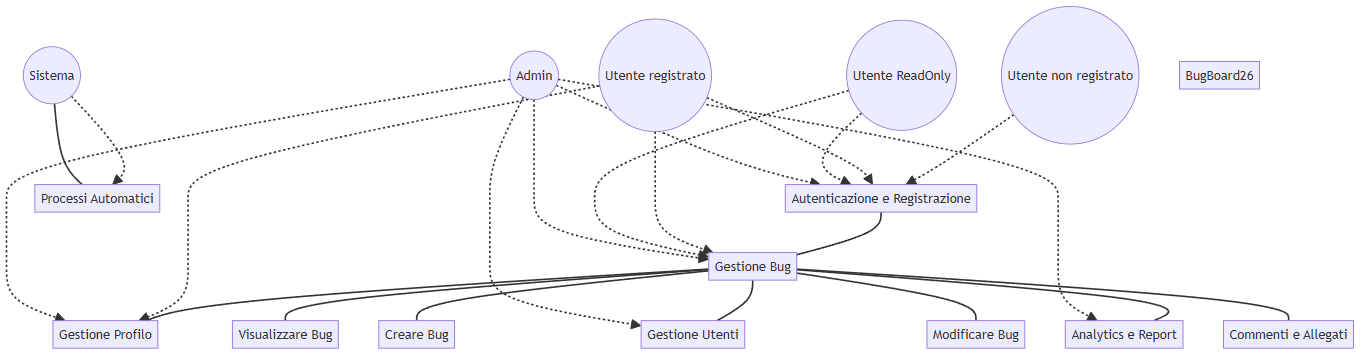
\includegraphics[width=0.82\textwidth,height=0.82\textheight,keepaspectratio]{diagramma_generale.png}
\caption{Diagramma generale dei casi d'uso --- BugBoard26}
\end{figure}

\subsubsection{Diagramma Dettagliato --- Gestione Bug}

\begin{figure}[H]
\centering
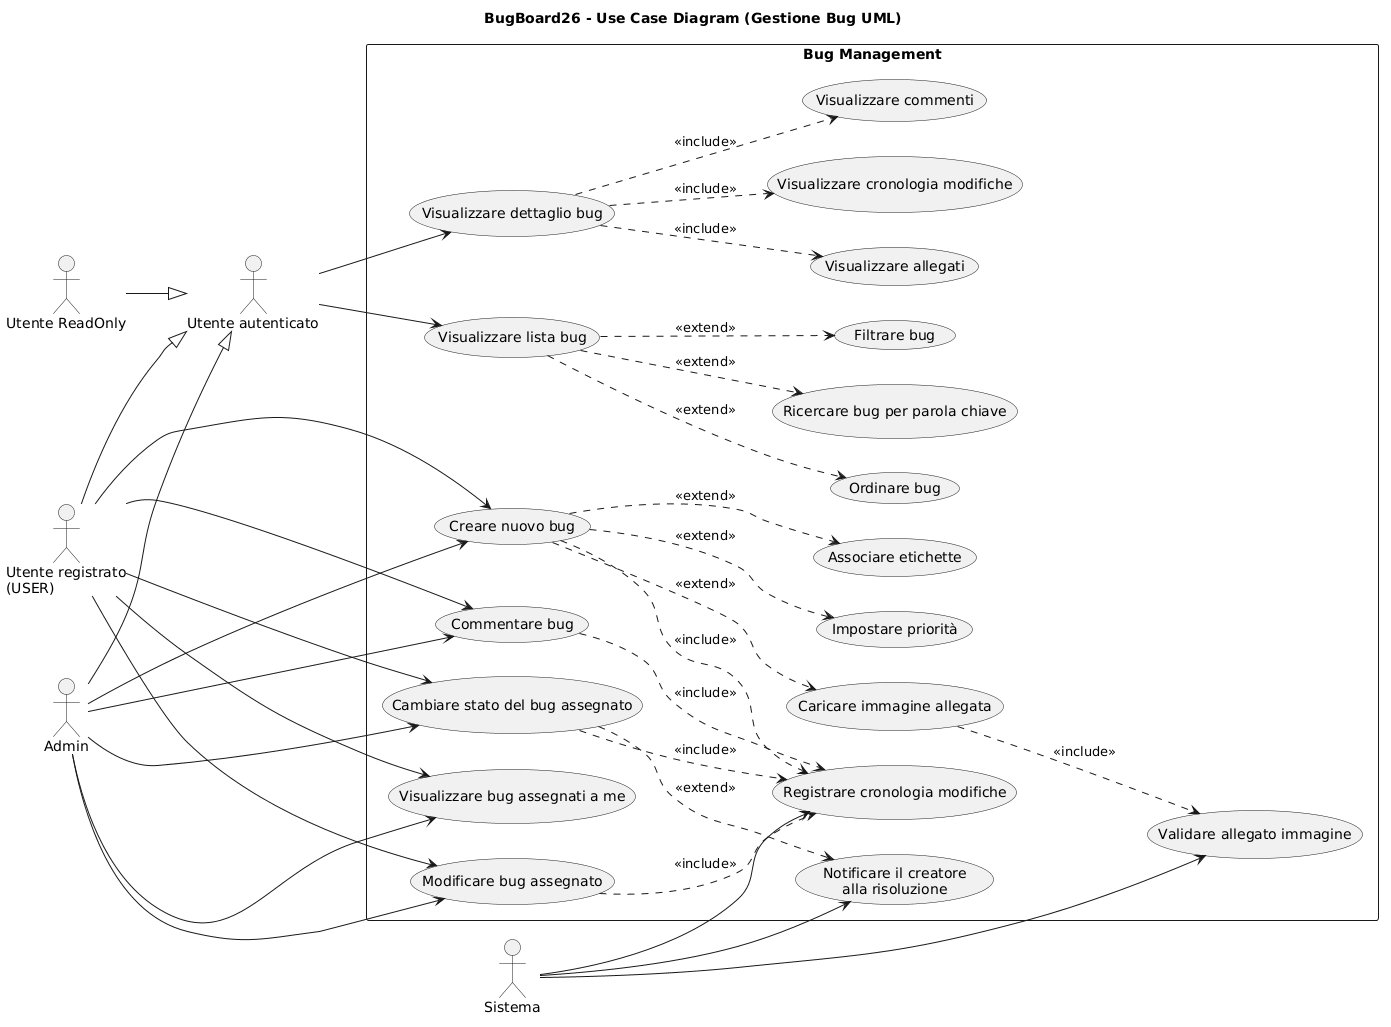
\includegraphics[width=0.85\textwidth]{diagramma_bug_management.png}
\caption{Diagramma dettagliato --- Gestione Bug}
\end{figure}

\subsubsection{Diagramma Dettagliato --- Amministrazione}

\begin{figure}[H]
\centering
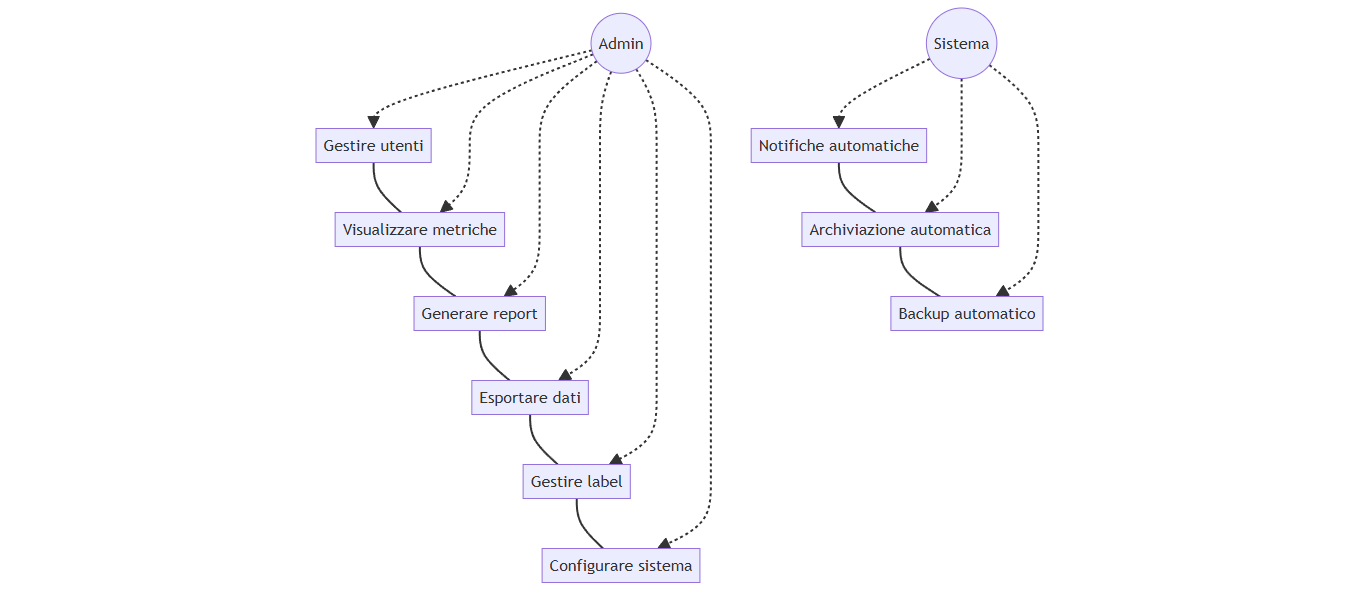
\includegraphics[width=0.85\textwidth]{diagramma_amministrazione.png}
\caption{Diagramma dettagliato --- Amministrazione e funzioni di sistema}
\end{figure}

\subsection{Convenzioni grafiche}
\begin{itemize}
  \item \textbf{Attori} (omino stilizzato o rettangolo): entit\`a esterne che interagiscono con il sistema
  \item \textbf{Casi d'uso} (ellissi): funzionalit\`a offerte dal sistema
  \item \textbf{Linee solide}: relazione di associazione tra attore e caso d'uso
  \item \textbf{Frecce tratteggiate $\ll$include$\gg$}: il caso d'uso base include sempre il caso d'uso puntato
  \item \textbf{Frecce tratteggiate $\ll$extend$\gg$}: il caso d'uso puntato estende opzionalmente il caso d'uso base
\end{itemize}

% ==================== 6. COCKBURN ====================
\section{Formalizzazione dei Casi d'Uso (Cockburn)}

In questa sezione vengono formalizzati quattro casi d'uso significativi, secondo il formalismo tabellare di Alistair Cockburn. Sono stati esclusi i casi d'uso relativi a registrazione e autenticazione, come indicato nelle istruzioni della traccia.

\subsection{Caso d'Uso 1: Creazione nuovo bug}

\begin{tabular}{|p{3cm}|p{11cm}|}
\hline
\textbf{Campo} & \textbf{Descrizione} \\
\hline
USE CASE \#01 & CREAZIONE NUOVO BUG \\
\hline
Goal & L'utente vuole segnalare un nuovo bug nel sistema \\
\hline
Preconditions & L'utente deve essere autenticato (ruolo USER o ADMIN) \\
\hline
Success End Condition & Il bug \`e creato con successo e registrato con un ID univoco \\
\hline
Failed End Condition & Il bug non viene creato a causa di errori di validazione o problemi di sistema \\
\hline
Primary Actor & Utente registrato (USER) \\
\hline
\end{tabular}

\vspace{0.5cm}

\begin{tabular}{|p{2cm}|p{5.5cm}|p{6.5cm}|}
\hline
\textbf{Flusso} & \textbf{Utente} & \textbf{Sistema} \\
\hline
Step 1 & Accede alla sezione ``Nuovo Bug'' & Mostra il form con i campi obbligatori \\
\hline
Step 2 & Inserisce il titolo del bug & Valida che il titolo non sia vuoto \\
\hline
Step 3 & Seleziona il tipo (Question, Bug, Documentation, Feature) & Carica le categorie disponibili \\
\hline
Step 4 & Inserisce la descrizione dettagliata & Fornisce un'area di testo \\
\hline
Step 5 & Seleziona la priorit\`a opzionale (Low, Medium, High, Urgent) & Mostra le opzioni con colori identificativi \\
\hline
Step 6 & Aggiunge label/tag opzionali & Permette selezione multipla da lista \\
\hline
Step 7 & Carica immagini allegati (opzionale) & Valida formato (JPEG, PNG, GIF, WebP) e dimensione (max 5\,MB) \\
\hline
Step 8 & Se previsto dal ruolo Admin, imposta una deadline opzionale & Mostra il selettore data solo agli utenti amministratori \\
\hline
Step 9 & Clicca su ``Crea Bug'' & Valida tutti i campi obbligatori \\
\hline
Step 10 & & Salva il bug nel database \\
\hline
Step 11 & & Registra la creazione nello storico delle modifiche \\
\hline
Step 12 & & Mostra conferma con l'ID del bug creato \\
\hline
\end{tabular}

\vspace{0.5cm}

\begin{tabular}{|p{3cm}|p{1.5cm}|p{9.5cm}|}
\hline
\textbf{EXTENSIONS} & \textbf{Step} & \textbf{Descrizione} \\
\hline
Caricamento immagini fallito & 7.a & Mostra errore ``Formato non supportato'' \\
\cline{2-3}
 & 7.b & L'utente pu\`o riprovare con file diverso \\
\hline
Validazione campi fallita & 9.a & Evidenzia i campi con errori \\
\cline{2-3}
 & 9.b & Mostra messaggi di errore per ciascun campo \\
\hline
Deadline non consentita al ruolo corrente & 8.a & Il campo non viene mostrato agli utenti non Admin \\
\cline{2-3}
 & 8.b & Il sistema ignora eventuali tentativi client-side di impostarla senza autorizzazione \\
\hline
\end{tabular}

\subsection{Caso d'Uso 2: Assegnazione bug a un utente}

\begin{tabular}{|p{3cm}|p{11cm}|}
\hline
\textbf{Campo} & \textbf{Descrizione} \\
\hline
USE CASE \#02 & ASSEGNAZIONE BUG A UN UTENTE \\
\hline
Goal & L'amministratore vuole assegnare o riassegnare un bug a un utente del sistema \\
\hline
Preconditions & L'utente deve essere autenticato con ruolo ADMIN; il bug deve esistere nel sistema \\
\hline
Success End Condition & Il bug risulta assegnato al nuovo utente e la modifica \`e registrata nello storico \\
\hline
Failed End Condition & L'assegnazione fallisce per utente di destinazione non valido \\
\hline
Primary Actor & Admin \\
\hline
\end{tabular}

\vspace{0.5cm}

\begin{tabular}{|p{2cm}|p{5.5cm}|p{6.5cm}|}
\hline
\textbf{Flusso} & \textbf{Utente (Admin)} & \textbf{Sistema} \\
\hline
Step 1 & Visualizza i dettagli di un bug & Mostra la pagina di dettaglio con tutte le informazioni \\
\hline
Step 2 & Clicca su ``Assegna'' & Apre il form di assegnazione \\
\hline
Step 3 & Visualizza la lista dei membri del team con carico di lavoro corrente & Evidenzia l'utente suggerito con meno bug assegnati \\
\hline
Step 4 & Seleziona l'utente dalla lista & Valida che l'utente esista e sia assegnabile \\
\hline
Step 5 & Clicca su ``Assegna'' & Verifica i permessi dell'utente richiedente e la presenza di una selezione valida \\
\hline
Step 6 & & Aggiorna il campo ``assegnato a'' nel database \\
\hline
Step 7 & & Registra la modifica nella tabella history \\
\hline
Step 8 & & Invia notifica al nuovo assegnatario \\
\hline
Step 9 & & Mostra messaggio di conferma e reindirizza al dettaglio del bug \\
\hline
\end{tabular}

\vspace{0.5cm}

\begin{tabular}{|p{3cm}|p{1.5cm}|p{9.5cm}|}
\hline
\textbf{EXTENSIONS} & \textbf{Step} & \textbf{Descrizione} \\
\hline
Utente non trovato & 4.a & Mostra errore ``Utente non esistente'' \\
\cline{2-3}
 & 4.b & L'admin pu\`o selezionare un altro membro del team \\
\hline
Nessun utente selezionato & 5.a & Mostra errore ``Seleziona un utente'' \\
\cline{2-3}
 & 5.b & L'assegnazione non viene inviata finch\'e non viene scelta una destinazione valida \\
\hline
\end{tabular}

\subsection{Caso d'Uso 3: Aggiornamento stato di un bug assegnato}

\begin{tabular}{|p{3cm}|p{11cm}|}
\hline
\textbf{Campo} & \textbf{Descrizione} \\
\hline
USE CASE \#03 & AGGIORNAMENTO STATO DI UN BUG ASSEGNATO \\
\hline
Goal & L'utente vuole aggiornare lo stato di un bug che pu\`o modificare \\
\hline
Preconditions & L'utente deve essere autenticato; deve essere Admin oppure assegnatario del bug \\
\hline
Success End Condition & Il bug viene salvato con il nuovo stato e la modifica viene registrata nello storico \\
\hline
Failed End Condition & L'aggiornamento fallisce per permessi insufficienti, dati non validi o bug inesistente \\
\hline
Primary Actor & Utente registrato (USER) assegnato al bug oppure Admin \\
\hline
\end{tabular}

\vspace{0.5cm}

\begin{tabular}{|p{2cm}|p{5.5cm}|p{6.5cm}|}
\hline
\textbf{Flusso} & \textbf{Utente} & \textbf{Sistema} \\
\hline
Step 1 & Visualizza i dettagli del bug assegnato & Mostra la pagina di dettaglio con lo stato attuale \\
\hline
Step 2 & Clicca su ``Modifica'' & Verifica che l'utente abbia i permessi per intervenire sul bug \\
\hline
Step 3 & & Mostra il form di modifica con i campi editabili \\
\hline
Step 4 & Aggiorna lo stato del bug (\emph{Todo}, \emph{In Progress}, \emph{Resolved}) & Valida il nuovo valore selezionato \\
\hline
Step 5 & Eventualmente modifica titolo, descrizione, priorit\`a o label & Mostra i campi consentiti dal ruolo corrente \\
\hline
Step 6 & Clicca su ``Salva'' & Valida i dati inviati \\
\hline
Step 7 & & Aggiorna il bug nel database \\
\hline
Step 8 & & Registra la modifica nella tabella history \\
\hline
Step 9 & & Se lo stato diventa \emph{Resolved}, invia una notifica al creatore del bug \\
\hline
Step 10 & & Mostra il dettaglio aggiornato del bug \\
\hline
\end{tabular}

\vspace{0.5cm}

\begin{tabular}{|p{3cm}|p{1.5cm}|p{9.5cm}|}
\hline
\textbf{EXTENSIONS} & \textbf{Step} & \textbf{Descrizione} \\
\hline
Permessi insufficienti & 2.a & Nega l'accesso alla modifica se l'utente non \`e Admin n\'e assegnatario \\
\cline{2-3}
 & 2.b & Mantiene il bug in sola lettura \\
\hline
Validazione campi fallita & 6.a & Evidenzia i campi obbligatori mancanti o non validi \\
\cline{2-3}
 & 6.b & Il salvataggio non viene completato finch\'e gli errori non sono corretti \\
\hline
Bug non trovato & 1.a & Mostra un messaggio di errore nel dettaglio \\
\cline{2-3}
 & 1.b & Interrompe il flusso di modifica \\
\hline
\end{tabular}

\subsection{Caso d'Uso 4: Consultazione report mensile (Admin)}

\begin{tabular}{|p{3cm}|p{11cm}|}
\hline
\textbf{Campo} & \textbf{Descrizione} \\
\hline
USE CASE \#04 & CONSULTAZIONE REPORT MENSILE \\
\hline
Goal & L'amministratore vuole consultare il report mensile dell'attivit\`a del sistema per un mese specifico \\
\hline
Preconditions & L'utente deve essere autenticato con ruolo ADMIN \\
\hline
Success End Condition & Il report del mese selezionato viene mostrato con metriche aggregate e dettaglio per utente \\
\hline
Failed End Condition & La generazione fallisce per assenza di dati nel periodo selezionato o errori di sistema \\
\hline
Primary Actor & Admin \\
\hline
\end{tabular}

\vspace{0.5cm}

\begin{tabular}{|p{2cm}|p{5.5cm}|p{6.5cm}|}
\hline
\textbf{Flusso} & \textbf{Utente (Admin)} & \textbf{Sistema} \\
\hline
Step 1 & Accede alla sezione ``Report Mensili'' & Mostra la schermata con il selettore del mese \\
\hline
Step 2 & Visualizza il mese corrente preimpostato oppure ne seleziona uno differente & Valida che il mese non sia futuro \\
\hline
Step 3 & Conferma la scelta del periodo tramite il campo mese & Richiede al backend i dati aggregati del mese selezionato \\
\hline
Step 4 & & Raccoglie dati dalle tabelle bugs, users e history \\
\hline
Step 5 & & Calcola metriche aggregate e medie di risoluzione \\
\hline
Step 6 & & Mostra card riepilogative e tabella di dettaglio per utente \\
\hline
Step 7 & Pu\`o scegliere ``Esporta report completo'' & Reindirizza alla sezione export per il download dei dati \\
\hline
\end{tabular}

\vspace{0.5cm}

\begin{tabular}{|p{3cm}|p{1.5cm}|p{9.5cm}|}
\hline
\textbf{EXTENSIONS} & \textbf{Step} & \textbf{Descrizione} \\
\hline
Report non disponibile & 3.a & Mostra un messaggio di errore per il mese selezionato \\
\cline{2-3}
 & 3.b & L'admin pu\`o selezionare un altro periodo \\
\hline
Errore nel caricamento & 4.a & Registra l'errore nel log \\
\cline{2-3}
 & 4.b & Mostra un messaggio di errore all'amministratore \\
\cline{2-3}
 & 4.c & Suggerisce di riprovare o selezionare un altro mese \\
\hline
\end{tabular}

% ==================== 7. REQUISITI NON FUNZIONALI ====================
\section{Requisiti Non Funzionali e di Sistema}

I requisiti non funzionali definiscono le caratteristiche qualitative che il sistema BugBoard26 deve possedere, indipendentemente dalle funzionalit\`a specifiche implementate.

\subsection{Usabilit\`a}
\begin{itemize}
  \item \textbf{RNF-U1 --- Interfaccia responsiva}: L'interfaccia deve essere fruibile su dispositivi desktop, tablet e mobile senza perdita di funzionalit\`a. Il layout si adatta automaticamente alla larghezza dello schermo.
  \item \textbf{RNF-U2 --- Feedback immediato}: Ogni operazione che richiede elaborazione (es.\ creazione bug, caricamento allegati) deve fornire un feedback visivo all'utente entro 500\,ms (es.\ spinner, messaggio di conferma o di errore).
  \item \textbf{RNF-U3 --- Messaggi di errore chiari}: I messaggi di errore devono indicare la causa del problema e suggerire un'azione correttiva, senza esporre dettagli tecnici interni.
  \item \textbf{RNF-U4 --- Accessibilit\`a}: L'interfaccia deve rispettare le linee guida WCAG 2.1 livello AA, garantendo contrasti adeguati e compatibilit\`a con tecnologie assistive.
\end{itemize}

\subsection{Prestazioni}
\begin{itemize}
  \item \textbf{RNF-P1 --- Tempo di risposta API}: Le richieste API standard (lista bug, dettaglio bug, login) devono avere un tempo di risposta inferiore a 500\,ms in condizioni normali di carico.
  \item \textbf{RNF-P2 --- Paginazione}: Il backend espone la lista bug in forma paginata (default 20 elementi per pagina) per contenere i dataset molto grandi; il frontend pu\`o aggregare pi\`u pagine quando deve offrire una vista continua all'utente.
  \item \textbf{RNF-P3 --- Dimensione allegati}: I file immagine caricati non possono superare 5\,MB ciascuno. Formati accettati: JPEG, PNG, GIF, WebP.
  \item \textbf{RNF-P4 --- Generazione report}: La generazione di un report mensile deve completarsi entro 10 secondi per dataset fino a 10\,000 bug.
\end{itemize}

\subsection{Sicurezza}
\begin{itemize}
  \item \textbf{RNF-S1 --- Autenticazione}: Tutti gli endpoint applicativi protetti richiedono un token JWT valido; restano pubblici solo login/logout e gli endpoint di supporto allo sviluppo (Swagger/H2). Il token ha una durata configurabile (default: 8 ore).
  \item \textbf{RNF-S2 --- Autorizzazione per ruolo}: Le operazioni privilegiate (gestione utenti, report, assegnazione bug) sono accessibili esclusivamente agli utenti con ruolo ADMIN.
  \item \textbf{RNF-S3 --- Validazione input}: Tutti i dati in input (lato client e lato server) sono validati prima dell'elaborazione. I file caricati sono verificati per tipo MIME e dimensione.
  \item \textbf{RNF-S4 --- Trasmissione sicura}: In produzione, tutte le comunicazioni tra client e server avvengono tramite HTTPS. I cookie di sessione sono configurati con i flag \texttt{Secure} e \texttt{SameSite}.
  \item \textbf{RNF-S5 --- Password}: Le password degli utenti sono memorizzate nel database in forma hash (bcrypt). Non vengono mai restituite nelle risposte API.
\end{itemize}

\subsection{Affidabilit\`a e Disponibilit\`a}
\begin{itemize}
  \item \textbf{RNF-A1 --- Gestione degli errori}: Il backend restituisce codici HTTP appropriati (400, 401, 403, 404, 500) con messaggi descrittivi. Il frontend mostra notifiche comprensibili per l'utente.
  \item \textbf{RNF-A2 --- Persistenza dei dati}: I dati sono persistiti su database relazionale (H2 in sviluppo, sostituibile con PostgreSQL in produzione). Nessuna operazione di scrittura avviene esclusivamente in memoria volatile.
  \item \textbf{RNF-A3 --- Storico immutabile}: La tabella \emph{History} non permette cancellazione o modifica dei record; ogni cambiamento genera un nuovo record.
\end{itemize}

\subsection{Manutenibilit\`a e Portabilit\`a}
\begin{itemize}
  \item \textbf{RNF-M1 --- Containerizzazione}: L'applicazione \`e distribuita tramite Docker (Dockerfile per frontend e backend; \texttt{docker-compose.yml} per l'avvio integrato).
  \item \textbf{RNF-M2 --- Separazione frontend/backend}: Frontend e backend sono componenti indipendenti che comunicano esclusivamente tramite API REST. Questa architettura consente di aggiornare o sostituire ciascun componente separatamente.
  \item \textbf{RNF-M3 --- Configurabilit\`a}: I parametri critici (URL del database, segreto JWT, porta del server, origine CORS) sono configurabili tramite variabili d'ambiente senza modificare il codice sorgente.
  \item \textbf{RNF-M4 --- Documentazione API}: Gli endpoint REST sono documentati tramite SpringDoc/OpenAPI (Swagger UI), accessibile in fase di sviluppo.
\end{itemize}

\subsection{Vincoli di Sistema}
\begin{itemize}
  \item \textbf{RNF-VS1 --- Tecnologie frontend}: React 18, TypeScript, Vite, Tailwind CSS, Radix UI, React Query, React Router.
  \item \textbf{RNF-VS2 --- Tecnologie backend}: Java 17, Spring Boot 3.3, Spring Security, Spring Data JPA, database H2 (sviluppo).
  \item \textbf{RNF-VS3 --- Browser supportati}: Le ultime due versioni stabili di Chrome, Firefox, Edge e Safari.
  \item \textbf{RNF-VS4 --- Requisiti server}: JDK 17+, Maven 3.8+, Node.js 18+ per la build del frontend.
\end{itemize}

% ==================== 8. MOCK-UP ====================
\section{Prototipazione visuale attraverso Mock-up}

La prototipazione visuale di BugBoard26 \`e stata realizzata in \textbf{Figma} attraverso un file condiviso di progetto, costruito prima con wireframe a bassa fedelt\`a e poi raffinato in mock-up ad alta fedelt\`a con componenti riutilizzabili, palette colori e varianti di stato. Le tavole esportate da Figma sono state usate come riferimento per l'implementazione React del prototipo funzionante e successivamente ricontrollate rispetto ai flussi effettivamente implementati.

\subsection{Scelte Progettuali}

\subsubsection{Layout e Navigazione}
\begin{itemize}
  \item \textbf{Navigazione principale persistente}: barra inferiore con accesso rapido a Home, lista bug, notifiche e profilo
  \item \textbf{Sezioni contestuali}: le schermate amministrative e di dettaglio presentano header locale con pulsante di ritorno e azioni disponibili nel contesto corrente
  \item \textbf{Layout responsive}: design \emph{mobile-first} realizzato con Tailwind CSS; le griglie si adattano automaticamente a qualsiasi larghezza schermo
\end{itemize}

\subsubsection{Palette Colori e Badge}
\begin{itemize}
  \item \textbf{Priorit\`a}: \emph{Urgent} (rosso), \emph{High} (arancione), \emph{Medium} (giallo), \emph{Low} (verde)
  \item \textbf{Stato}: \emph{Todo} (grigio chiaro), \emph{In Progress} (blu), \emph{Resolved} (verde), \emph{Archived} (grigio scuro)
  \item \textbf{Tipo}: \emph{Bug} (rosso), \emph{Feature} (viola), \emph{Question} (azzurro), \emph{Documentation} (grigio)
  \item \textbf{Azioni primarie}: blu (\#007BFF); superfici neutre: grigi Tailwind
\end{itemize}

\subsubsection{Componenti UI riutilizzati}
Tutti i componenti sono basati su \textbf{Radix UI} e \textbf{shadcn/ui}: Button, Card, Select, Dialog, Badge, Table, Toast, DropdownMenu. Questo garantisce coerenza visiva e accessibilit\`a WCAG 2.1 out-of-the-box.

\subsection{Mock-up delle interfacce utente}

Di seguito sono illustrate le schermate principali del prototipo, raggruppate per funzionalit\`a. Le schermate contrassegnate con \textbf{[UC0X]} corrispondono direttamente ai casi d'uso formalizzati nella sezione precedente.

\subsubsection{Mock-up 1 --- Pagina di Login}

\begin{figure}[H]
\centering
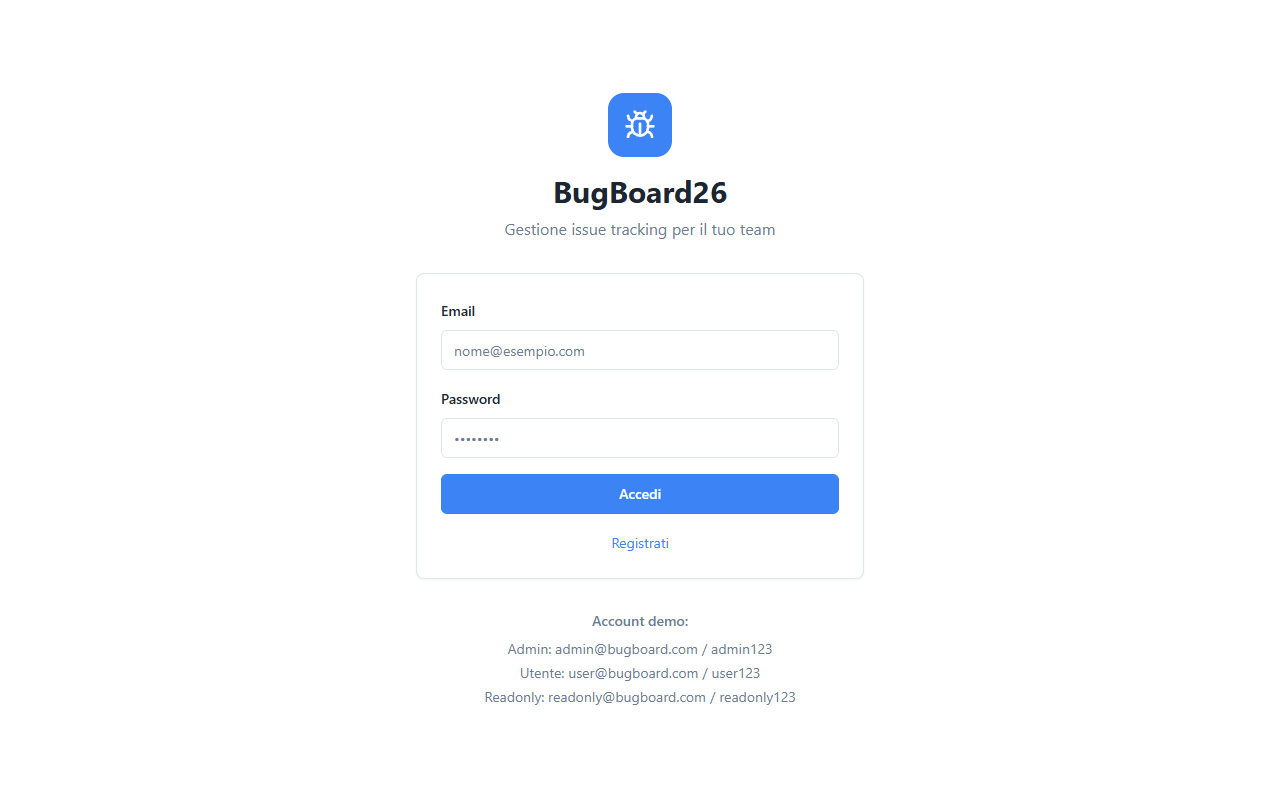
\includegraphics[width=0.7\textwidth]{mockup_01_login.png}
\caption{Pagina di Login: form con email e password, pulsante di accesso}
\end{figure}

\begin{itemize}
  \item \textbf{Scopo}: autenticazione dell'utente al sistema
  \item \textbf{Elementi}: campo email, campo password, pulsante ``Accedi'', link alla pagina informativa del progetto
  \item \textbf{Comportamento}: in caso di credenziali errate viene mostrato un messaggio di errore inline; in caso di successo l'utente viene reindirizzato alla Dashboard
\end{itemize}

\subsubsection{Mock-up 2 --- Pagina Informativa Richiesta Account}

\begin{figure}[H]
\centering
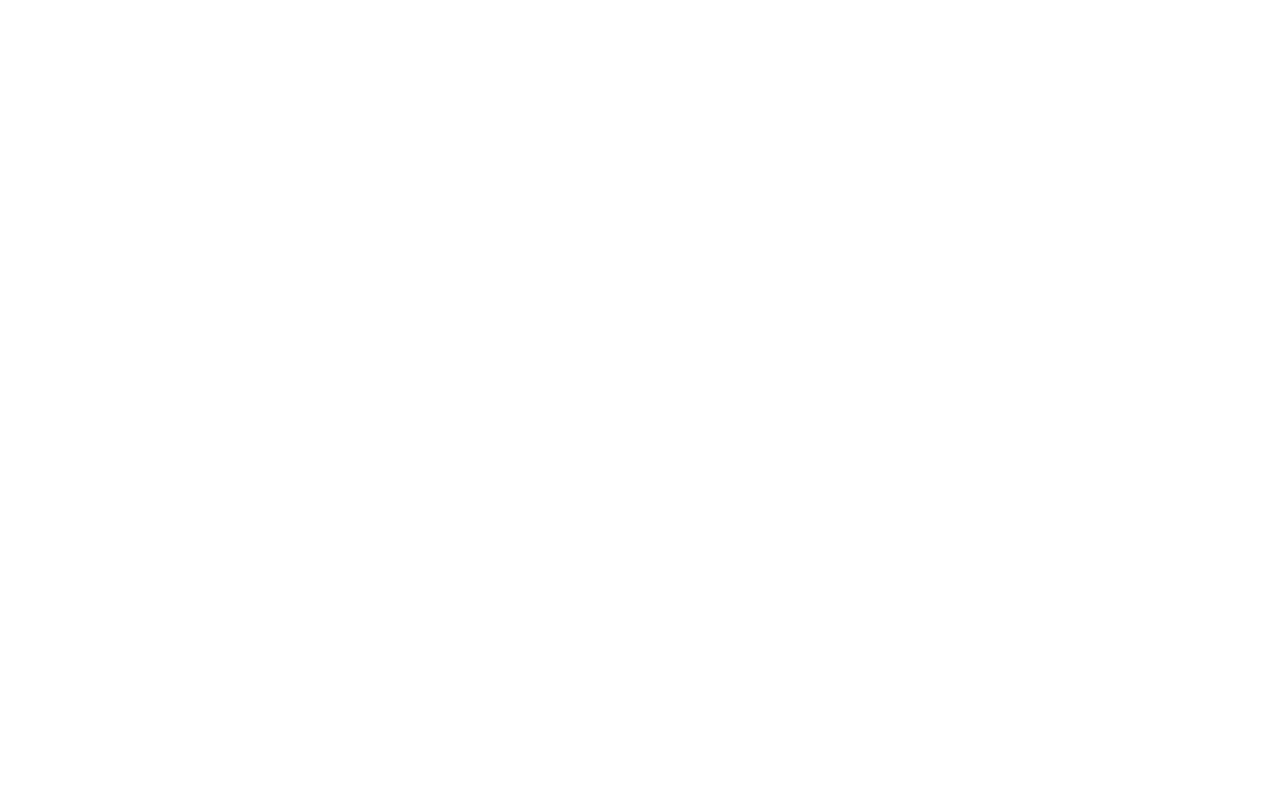
\includegraphics[width=0.7\textwidth]{mockup_02_register.png}
\caption{Pagina Informativa: indicazioni per l'accesso al sistema e richiesta di un account}
\end{figure}

\begin{itemize}
  \item \textbf{Scopo}: presentare il progetto e spiegare come ottenere un account creato da un amministratore
  \item \textbf{Elementi}: testo descrittivo, contatti o istruzioni per richiedere l'accesso, link al login
  \item \textbf{Comportamento}: nessuna registrazione self-service; l'utente viene indirizzato verso il canale corretto per la creazione dell'account
\end{itemize}

\subsubsection{Mock-up 3 --- Home / Dashboard}

\begin{figure}[H]
\centering
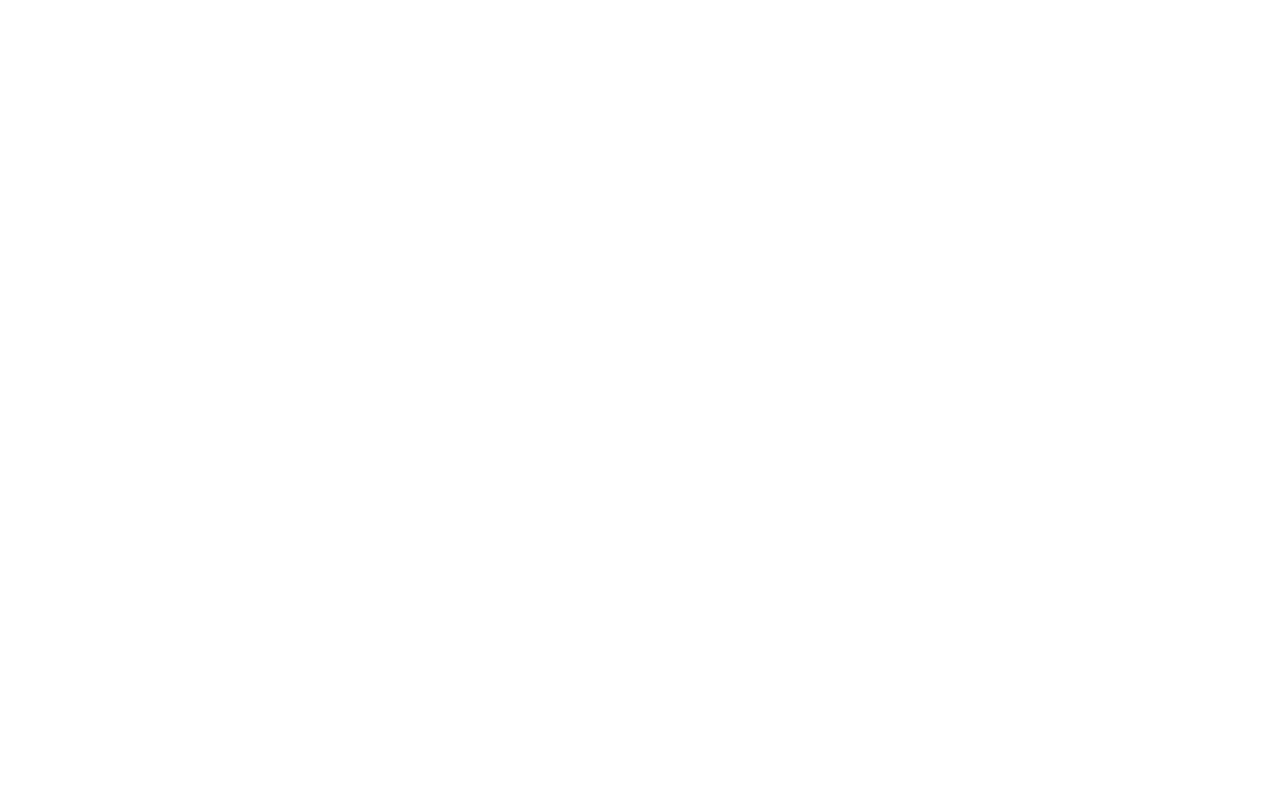
\includegraphics[width=0.7\textwidth]{mockup_03_home_dashboard.png}
\caption{Home Dashboard: panoramica delle metriche principali e accessi rapidi}
\end{figure}

\begin{itemize}
  \item \textbf{Scopo}: fornire una panoramica immediata dello stato del sistema dopo il login
  \item \textbf{Elementi}: card riepilogative delle metriche principali, saluto iniziale e area ``Azioni rapide''
  \item \textbf{Accessi rapidi}: da qui si pu\`o navigare alla lista bug, al form di creazione e, per gli Admin, alla gestione utenti
\end{itemize}

\subsubsection{Mock-up 4 --- Lista Bug con Filtri}

\begin{figure}[H]
\centering
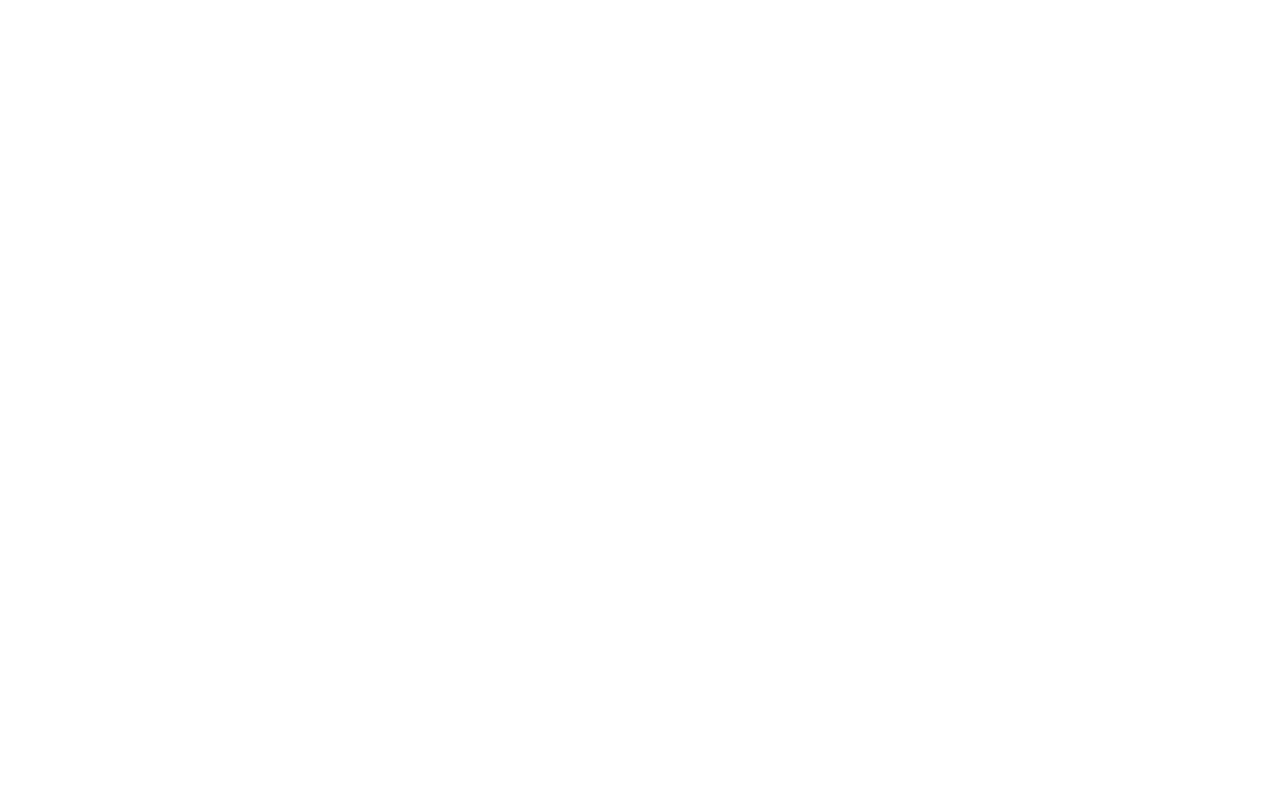
\includegraphics[width=0.7\textwidth]{mockup_04_lista_bug.png}
\caption{Lista Bug: elenco di card filtrabili per tipo, stato, priorit\`a e ricerca testuale}
\end{figure}

\begin{itemize}
  \item \textbf{Scopo}: visualizzazione e filtraggio dell'elenco completo dei bug
  \item \textbf{Elementi}: tab ``Tutti / Assegnati a me / Archiviati'', barra filtri orizzontale, campo ricerca full-text, card bug con badge colorati
  \item \textbf{Interazione}: il clic su una card apre il dettaglio del bug; i filtri si applicano in tempo reale e il frontend ricompone le pagine restituite dal backend
\end{itemize}

\subsubsection{Mock-up 5 --- Dettaglio Bug}

\begin{figure}[H]
\centering
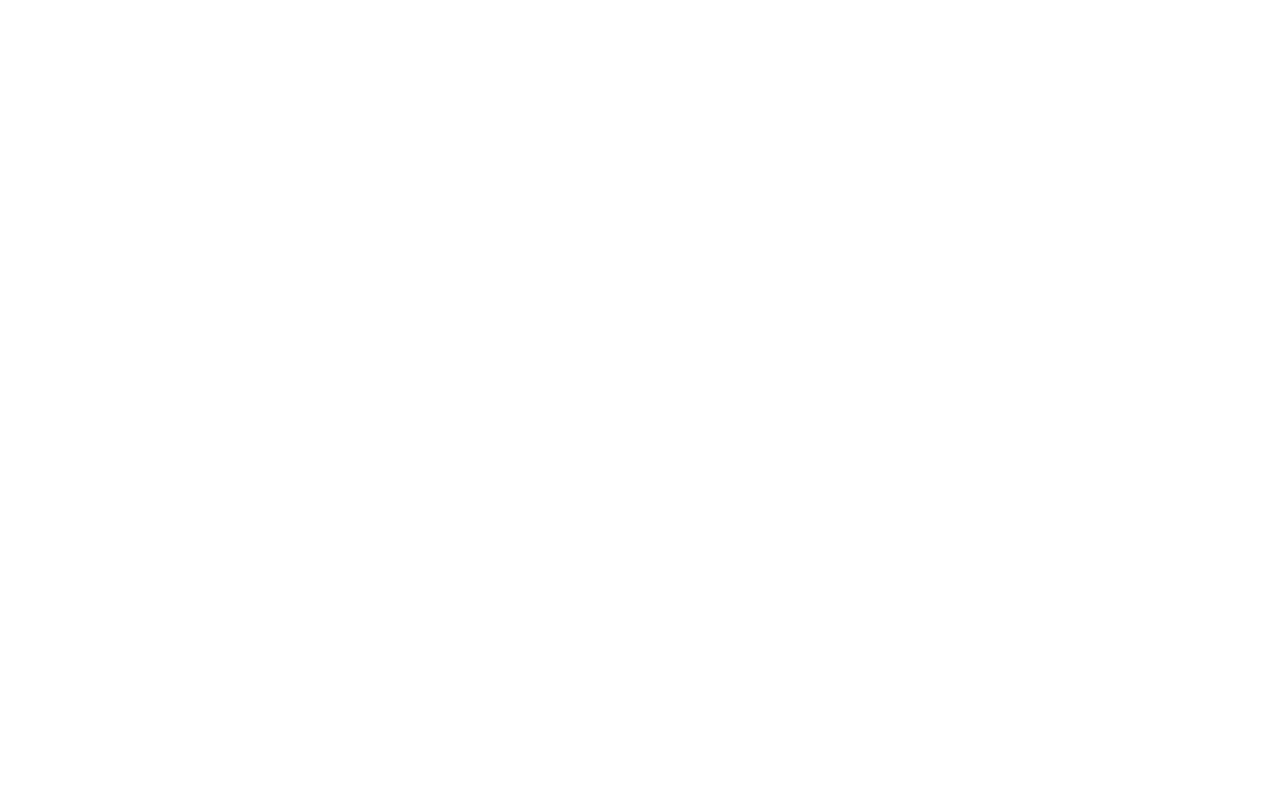
\includegraphics[width=0.7\textwidth]{mockup_05_dettaglio_bug.png}
\caption{Dettaglio Bug: informazioni complete, commenti, storico modifiche e azioni disponibili}
\end{figure}

\begin{itemize}
  \item \textbf{Scopo}: visualizzazione completa di un bug specifico e gestione delle azioni disponibili
  \item \textbf{Elementi}: header con breadcrumb locale, titolo, stato e priorit\`a; sezioni descrizione, dettagli, etichette, allegati, commenti e storico; barra azioni orizzontale sticky (modifica, assegna, archivia, duplica, esporta)
  \item \textbf{Azioni visibili}: dipendono dal ruolo dell'utente e dai permessi sul bug corrente
\end{itemize}

\subsubsection{Mock-up 6 --- Form Creazione/Modifica Bug \textbf{[UC01]}}

\begin{figure}[H]
\centering
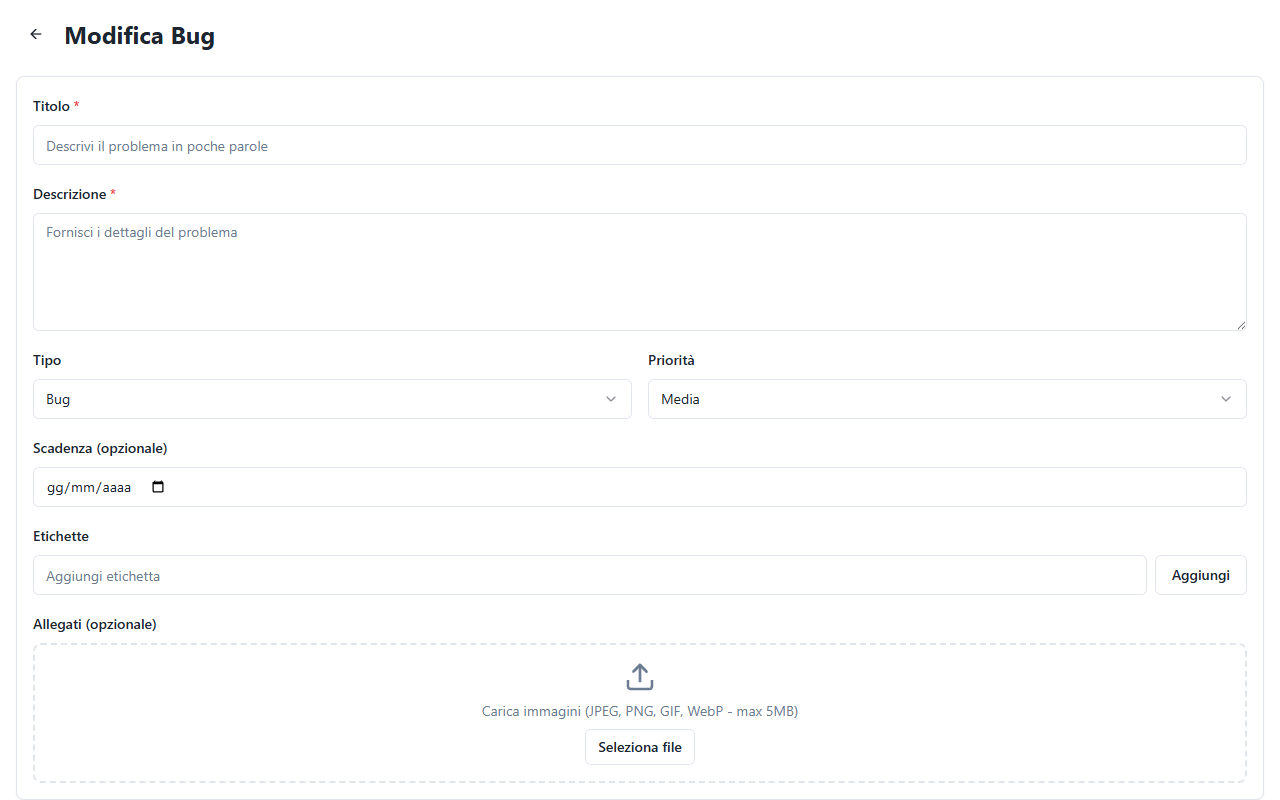
\includegraphics[width=0.7\textwidth]{mockup_06_form_creazione_bug.png}
\caption{Form Creazione Bug (UC01): campi titolo, tipo, priorit\`a opzionale, descrizione, label, allegati}
\end{figure}

\begin{itemize}
  \item \textbf{Caso d'uso}: UC01 --- Creazione nuovo bug
  \item \textbf{Elementi}: campo titolo, selettore tipo, selettore priorit\`a opzionale, area di testo descrizione, selezione label multipla, upload allegati immagine, pulsante ``Salva''; il campo deadline compare solo per Admin
  \item \textbf{Validazione}: i campi obbligatori (titolo e descrizione) sono evidenziati se lasciati vuoti; priorit\`a e allegati sono opzionali, mentre formato e dimensione degli allegati sono verificati prima dell'invio
\end{itemize}

\subsubsection{Mock-up 7 --- Assegnazione Bug \textbf{[UC02]}}

\begin{figure}[H]
\centering
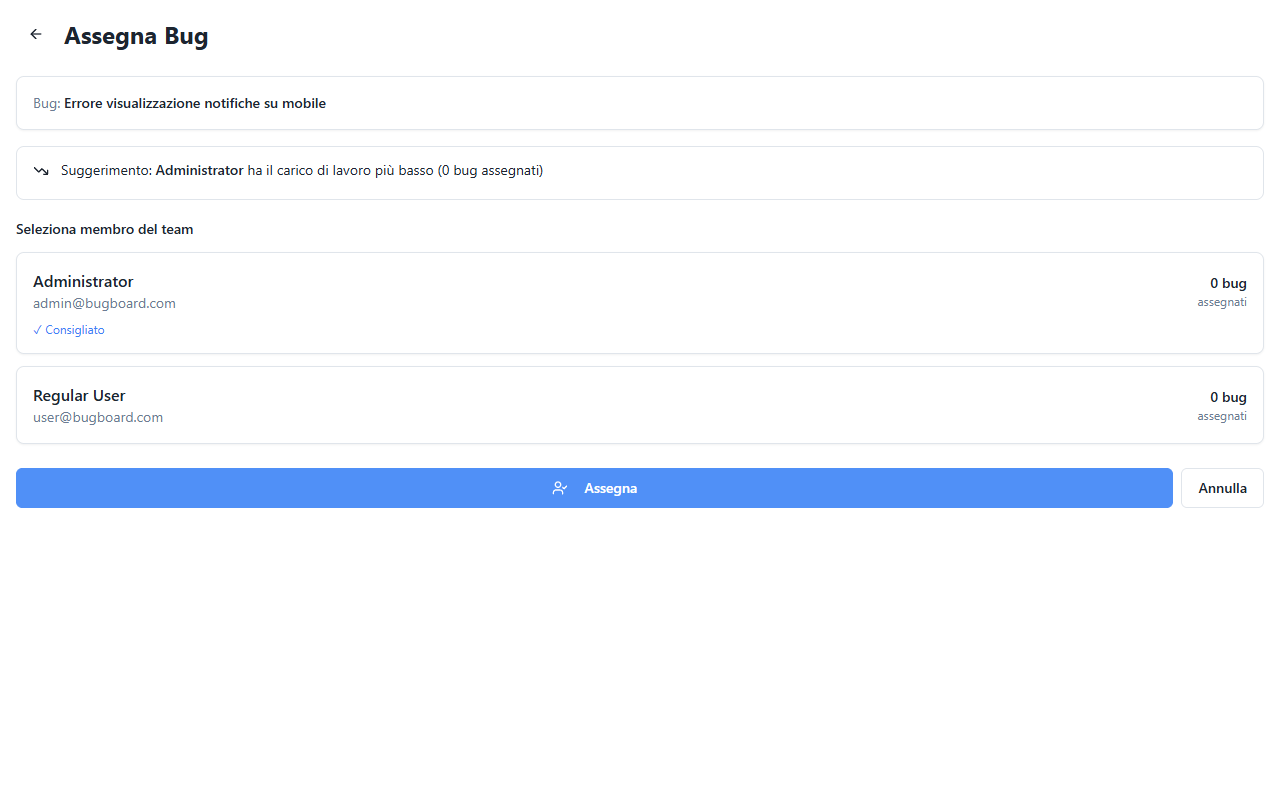
\includegraphics[width=0.7\textwidth]{mockup_07_assegnazione_bug.png}
\caption{Assegnazione Bug (UC02): selezione dell'utente a cui assegnare il bug}
\end{figure}

\begin{itemize}
  \item \textbf{Caso d'uso}: UC02 --- Assegnazione bug a un utente (solo Admin)
  \item \textbf{Elementi}: select per la scelta dell'utente assegnatario, pulsante conferma
  \item \textbf{Accesso}: questa schermata \`e accessibile solo agli utenti con ruolo Admin; un USER viene reindirizzato alla Dashboard
\end{itemize}

\subsubsection{Mock-up 8 --- Notifiche}

\begin{figure}[H]
\centering
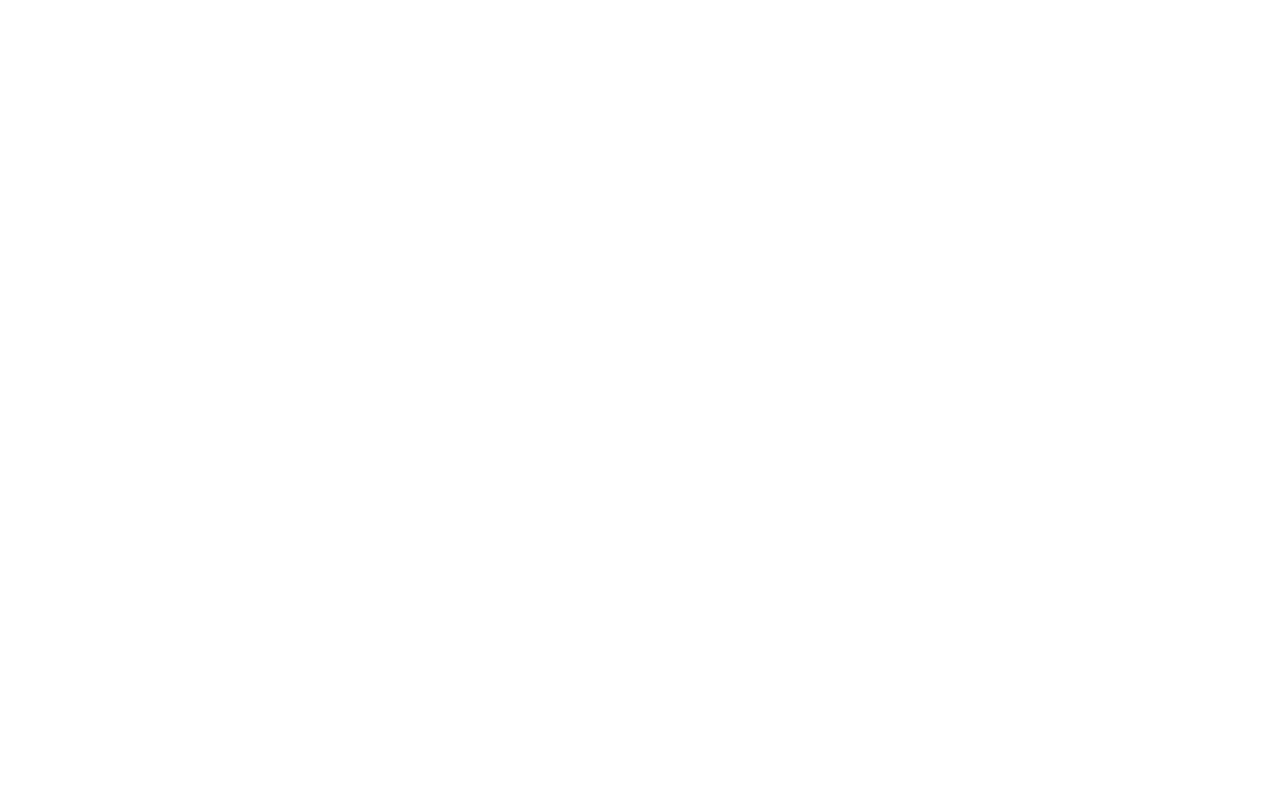
\includegraphics[width=0.7\textwidth]{mockup_08_notifiche.png}
\caption{Centro Notifiche: lista degli aggiornamenti sui bug seguiti dall'utente}
\end{figure}

\begin{itemize}
  \item \textbf{Scopo}: mostrare all'utente gli aggiornamenti recenti sui bug che lo riguardano (assegnazioni, cambi stato, nuovi commenti)
  \item \textbf{Elementi}: lista notifiche con timestamp, tipo evento e link al bug correlato; indicatore notifiche non lette
\end{itemize}

\subsubsection{Mock-up 9 --- Profilo Utente}

\begin{figure}[H]
\centering
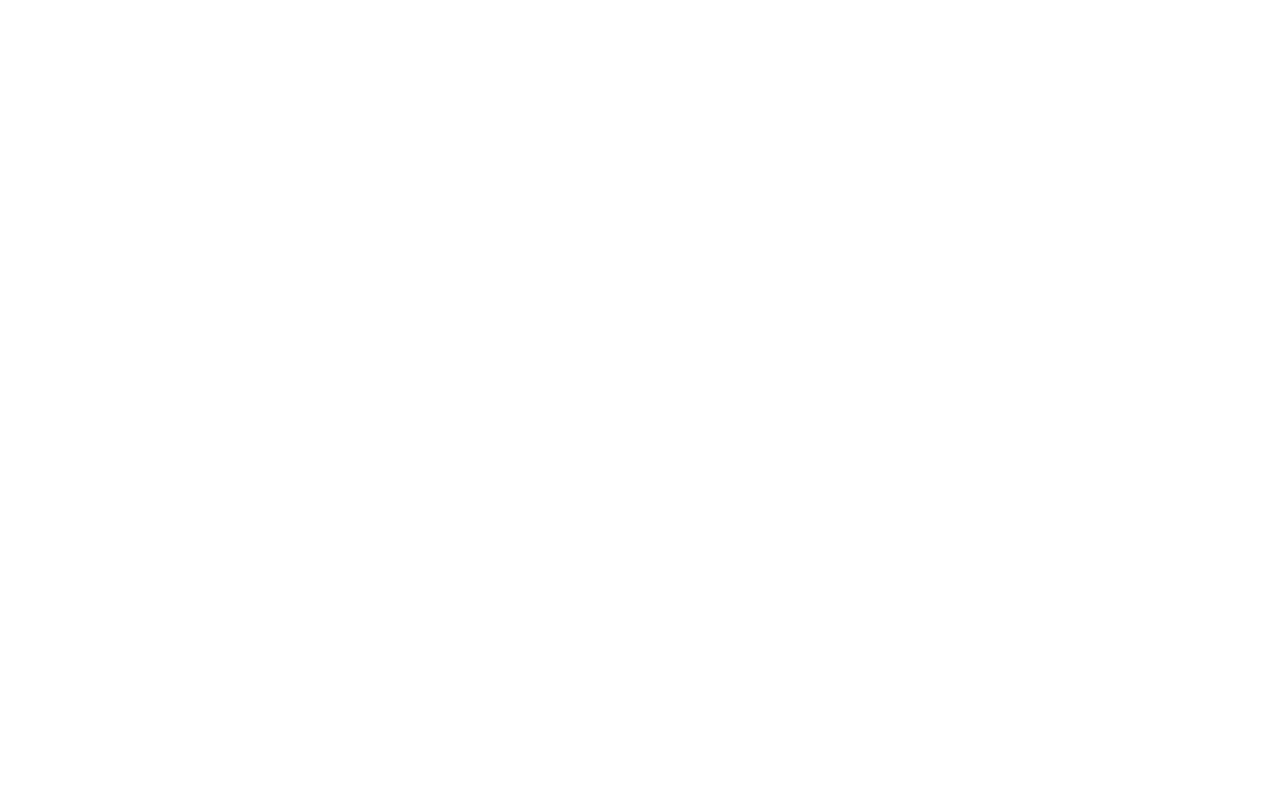
\includegraphics[width=0.7\textwidth]{mockup_09_profilo.png}
\caption{Profilo Utente: consultazione dati account e accesso alle sezioni personali}
\end{figure}

\begin{itemize}
  \item \textbf{Scopo}: consentire all'utente di consultare i dati del proprio account e raggiungere rapidamente le funzioni personali disponibili
  \item \textbf{Elementi}: nome, email, ruolo, ID utente, scorciatoie a export e modalit\`a sola lettura; per gli Admin compaiono anche collegamenti a gestione utenti, report e archivio
\end{itemize}

\subsubsection{Mock-up 10 --- Report Mensile \textbf{[UC04]}}

\begin{figure}[H]
\centering
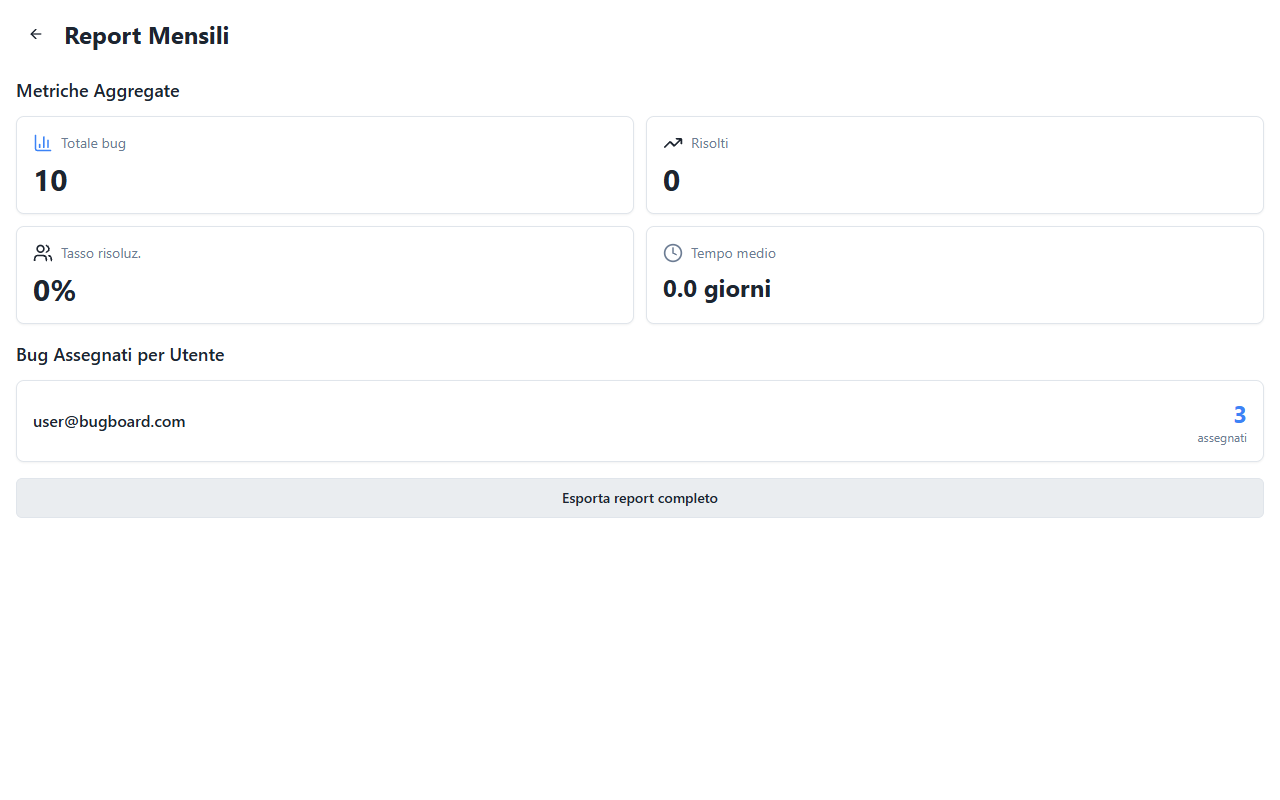
\includegraphics[width=0.7\textwidth]{mockup_10_report_mensile.png}
\caption{Report Mensile Admin (UC04): consultazione delle statistiche aggregate del mese e dettaglio per utente}
\end{figure}

\begin{itemize}
  \item \textbf{Caso d'uso}: UC04 --- Consultazione report mensile (solo Admin)
  \item \textbf{Elementi}: selettore mese, statistiche aggregate, tabella riassuntiva per utente e collegamento alla sezione export
  \item \textbf{Accesso}: solo Admin; gli altri utenti vengono reindirizzati alla Dashboard
\end{itemize}

\subsubsection{Mock-up 11 --- Gestione Utenti (Admin)}

\begin{figure}[H]
\centering
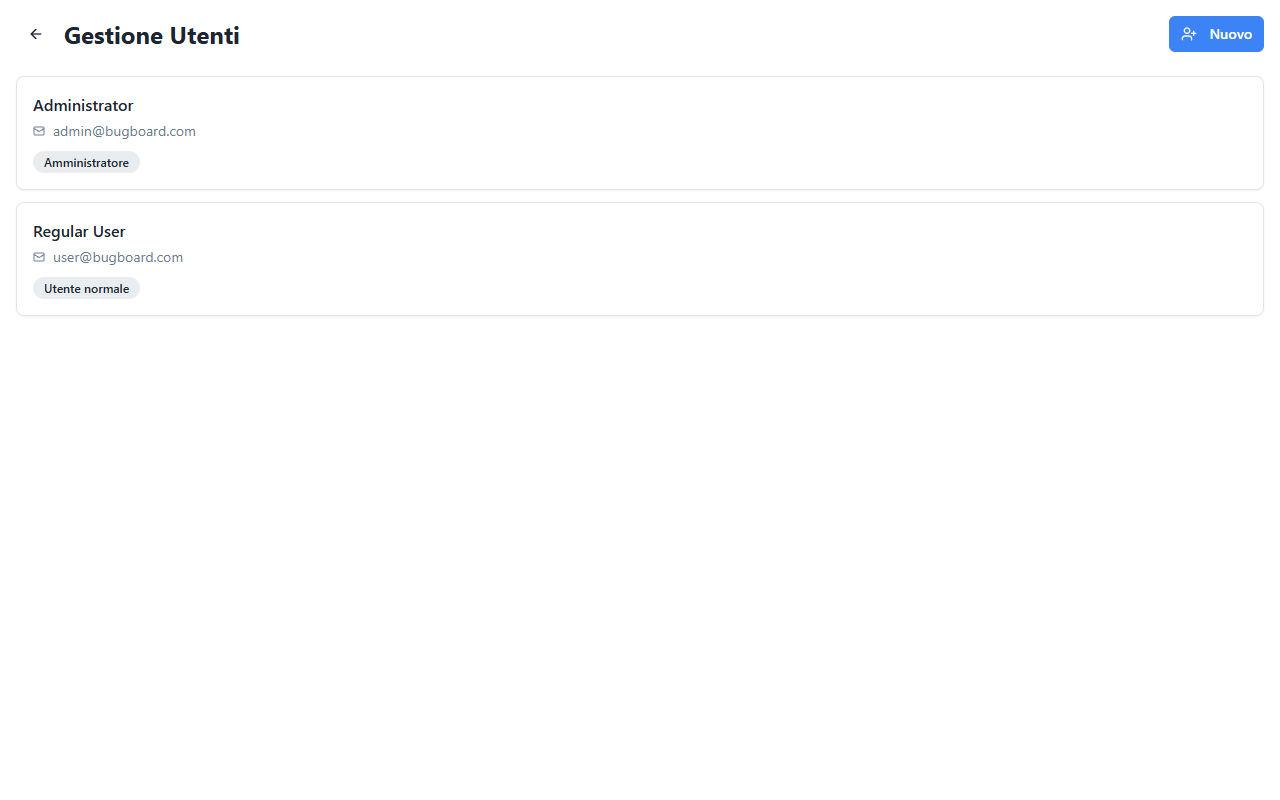
\includegraphics[width=0.7\textwidth]{mockup_11_admin_utenti.png}
\caption{Gestione Utenti Admin: lista utenti con ruoli e form di creazione account}
\end{figure}

\begin{itemize}
  \item \textbf{Scopo}: permettere all'Admin di gestire gli account del sistema tramite visualizzazione utenti e creazione di nuovi account con ruolo
  \item \textbf{Elementi}: tabella utenti con email, nome e ruolo; form per creazione di nuovi account Admin, User o ReadOnly
\end{itemize}

\subsubsection{Mock-up 12 --- Archivio Bug}

\begin{figure}[H]
\centering
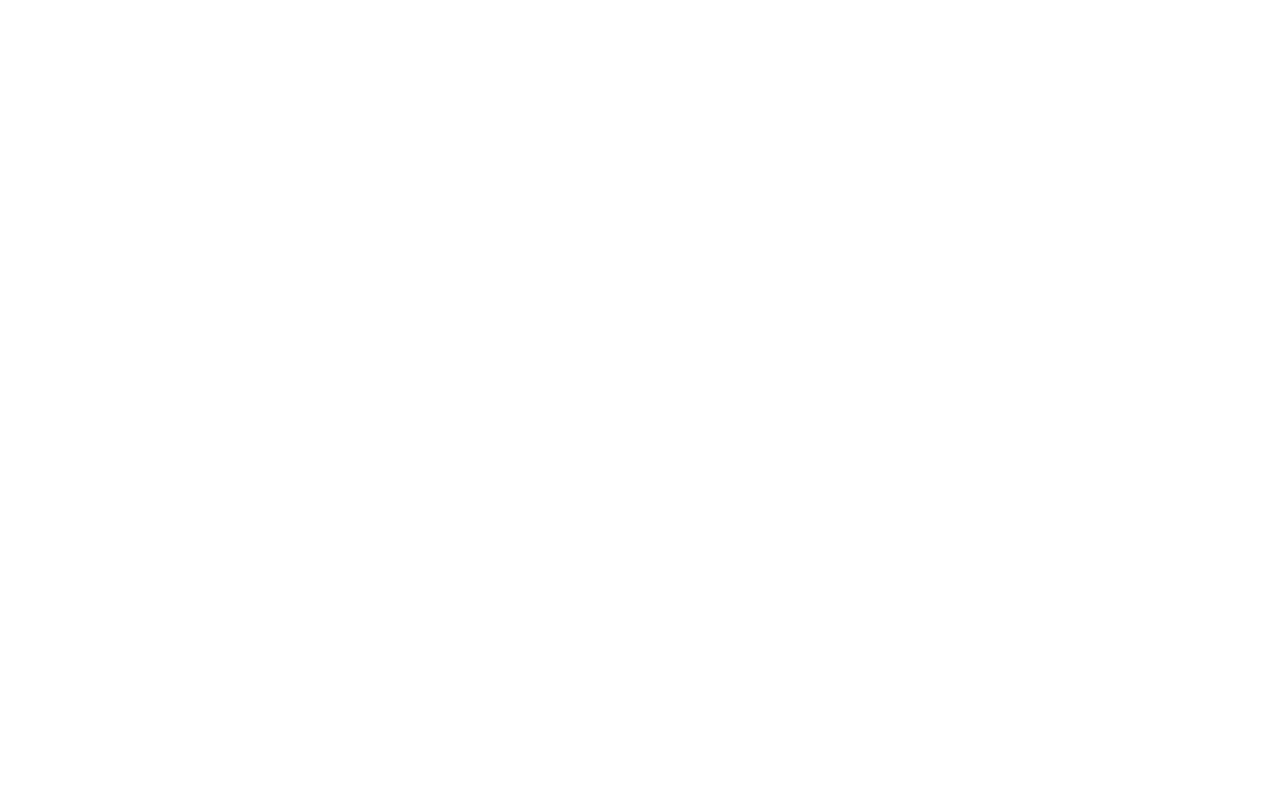
\includegraphics[width=0.7\textwidth]{mockup_12_archivio.png}
\caption{Archivio Bug: lista dei bug archiviati con possibilit\`a di consultazione}
\end{figure}

\begin{itemize}
  \item \textbf{Scopo}: visualizzare i bug archiviati per storico e consultazione senza influire sulla lista attiva
  \item \textbf{Elementi}: elenco dei bug in stato \emph{Archived} con ricerca; solo Admin pu\`o accedere alla sezione e archiviare manualmente i bug dalla vista di dettaglio
\end{itemize}

\subsubsection{Mock-up 13 --- Export Dati}

\begin{figure}[H]
\centering
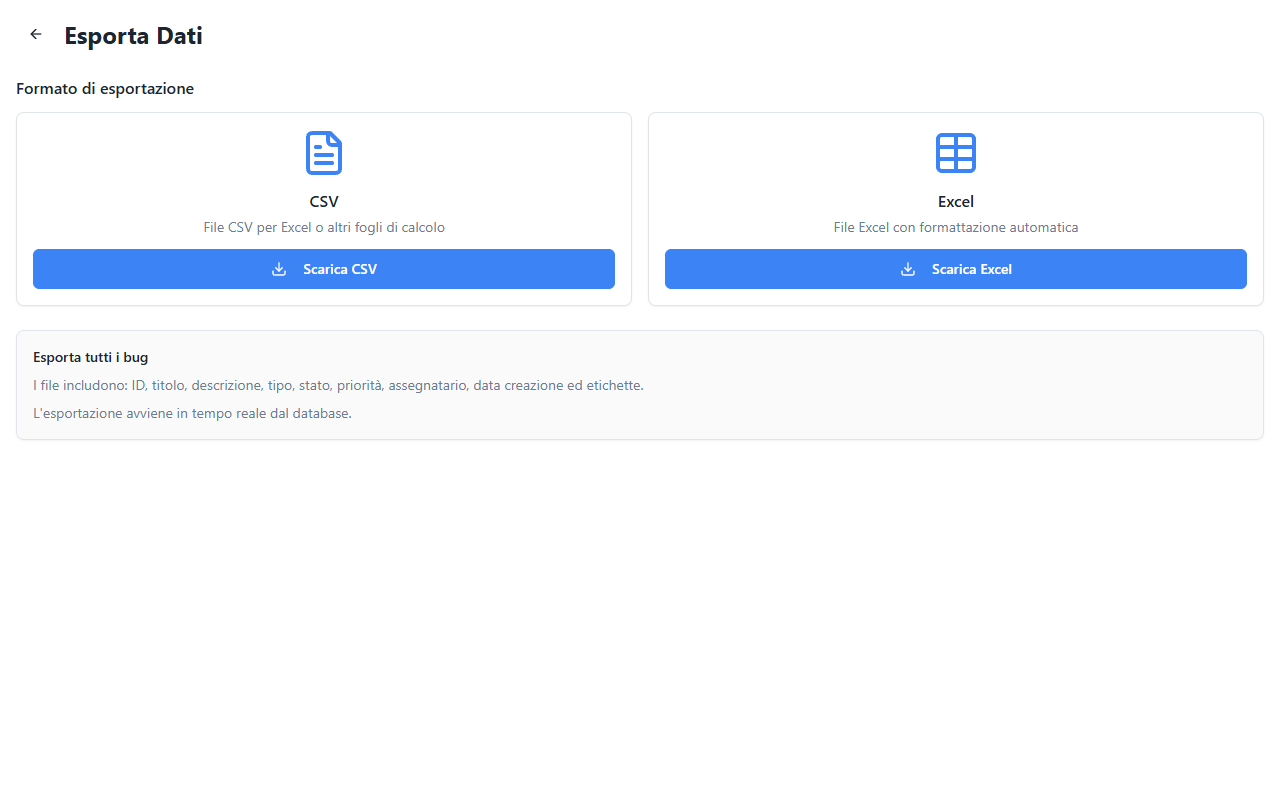
\includegraphics[width=0.7\textwidth]{mockup_13_export.png}
\caption{Export Dati: schermata di esportazione con opzioni CSV ed Excel; il PDF \`e supportato nella versione implementata}
\end{figure}

\begin{itemize}
  \item \textbf{Scopo}: consentire l'esportazione dei dati per analisi esterne
  \item \textbf{Elementi}: pulsanti ``Scarica CSV'' e ``Scarica Excel'' visibili nel mock-up; nella versione implementata la stessa pagina espone anche il download PDF
\end{itemize}

\subsection{Osservazioni emerse dalla prototipazione}

La costruzione dei mock-up in Figma e la loro successiva validazione sul prototipo funzionante hanno permesso di identificare alcune scelte migliorative rispetto all'analisi iniziale:

\begin{itemize}
  \item \textbf{Chiarezza dei ruoli}: \`e stato necessario rendere esplicito nel UI quali azioni sono riservate all'Admin (assegnazione, report, gestione utenti), aggiungendo reindirizzamenti automatici per utenti non autorizzati
  \item \textbf{Filtri immediati}: la lista bug con filtri in tempo reale si \`e rivelata la funzionalit\`a pi\`u usata nelle sessioni di test, confermando la scelta di renderla la pagina principale
  \item \textbf{Badge colorati}: l'uso di badge cromatici per stato, priorit\`a e tipo ha migliorato significativamente la leggibilit\`a della lista bug senza aprire il dettaglio
  \item \textbf{Navigazione mobile}: l'adozione di una bottom navigation persistente ha reso pi\`u immediato l'accesso alle sezioni principali sui dispositivi mobili
\end{itemize}

% ==================== 9. DESIGN DEL SISTEMA ====================
\section{Design del Sistema}

\subsection{Descrizione dell'architettura}

BugBoard26 adotta un'architettura \textbf{client-server a tre livelli} (Three-Tier Architecture), separando nettamente le responsabilit\`a tra \emph{presentazione}, \emph{logica di business} e \emph{persistenza dei dati}.

\begin{tabular}{|l|p{10cm}|}
\hline
\textbf{Livello} & \textbf{Descrizione} \\
\hline
Presentazione (Frontend) & Single Page Application React che comunica con il backend tramite API REST. \\
\hline
Logica di Business (Backend) & Applicazione Spring Boot che espone endpoint RESTful, gestisce autenticazione JWT e implementa le regole di business. \\
\hline
Persistenza (Database) & Database relazionale (H2 in sviluppo, PostgreSQL in produzione) gestito tramite JPA/Hibernate. \\
\hline
\end{tabular}

\subsubsection{Deployment Diagram}

\begin{figure}[H]
\centering
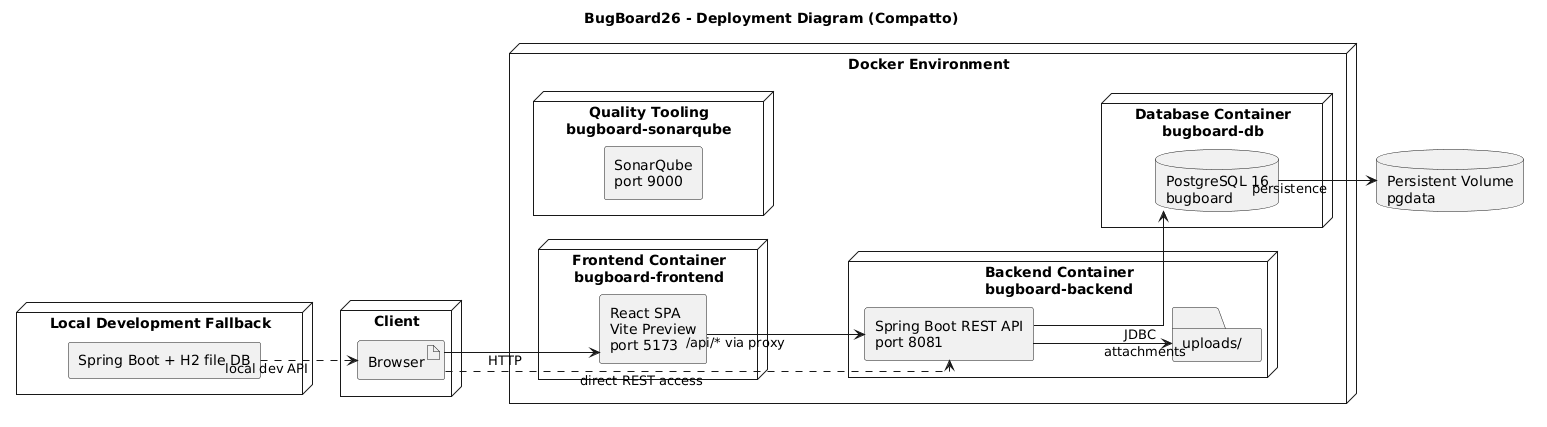
\includegraphics[width=\textwidth]{deployment_diagram.png}
\caption{Deployment Diagram --- BugBoard26}
\end{figure}

Il deployment diagram mostra la distribuzione fisica dei componenti tra i container Docker e l'ambiente di sviluppo locale.

\subsubsection{Component Diagram}

\begin{figure}[H]
\centering
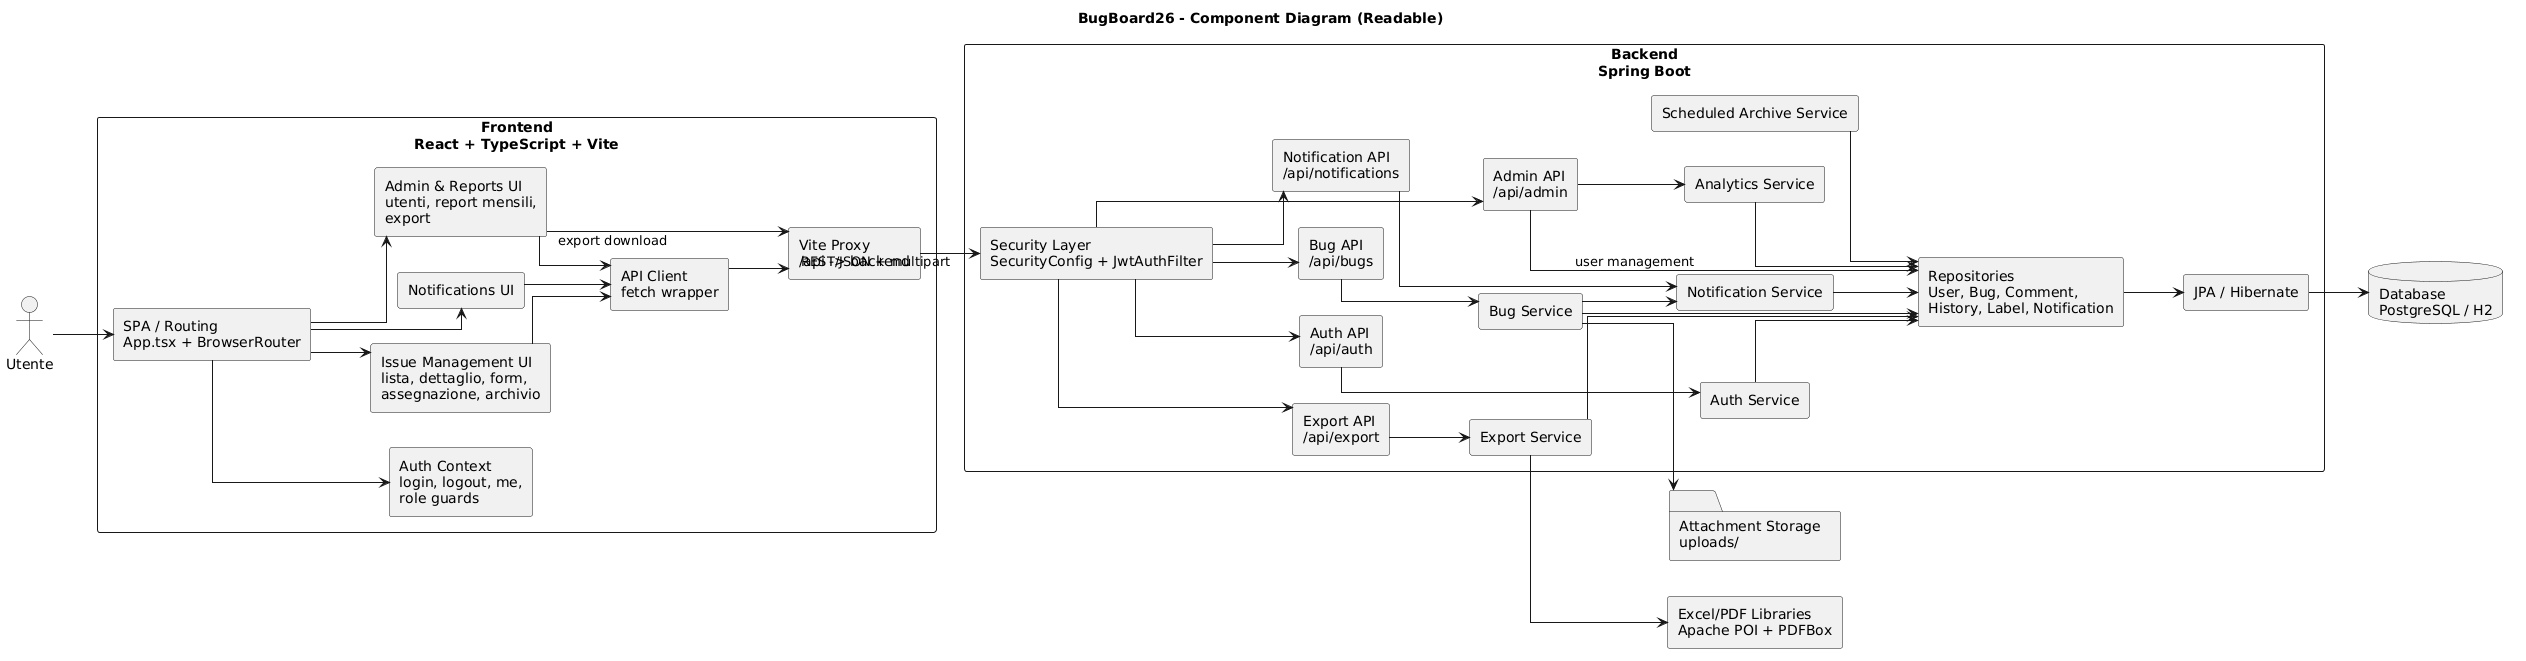
\includegraphics[width=\textwidth]{component_diagram.png}
\caption{Component Diagram --- BugBoard26}
\end{figure}

Il component diagram illustra i componenti software del sistema e le loro dipendenze, organizzati per layer architetturale.

\subsubsection{Diagrammi di approfondimento architetturale}

Accanto ai diagrammi sintetici principali, sono stati inclusi anche diagrammi UML pi\`u dettagliati, utili per descrivere con maggior precisione i layer interni del backend e le dipendenze effettivamente presenti nel repository.

\begin{figure}[H]
\centering
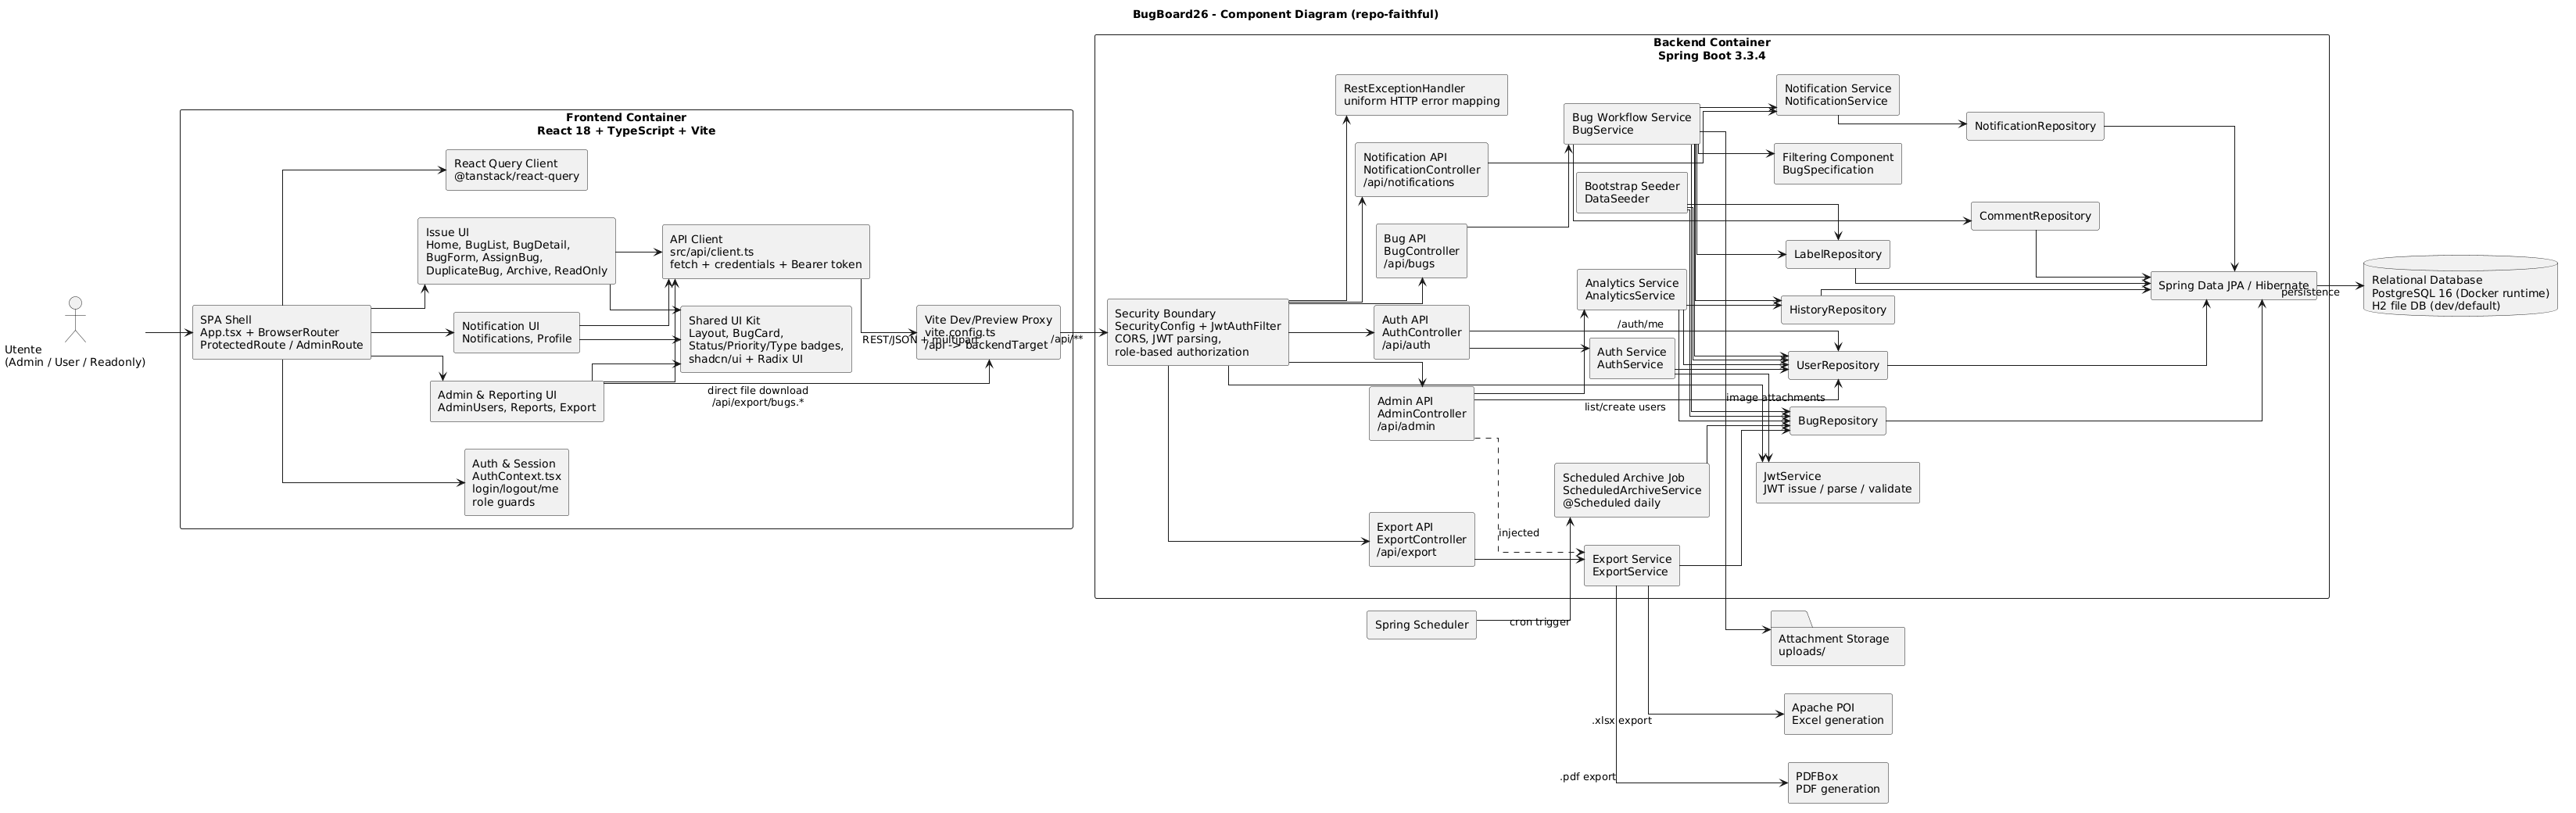
\includegraphics[width=\textwidth,height=0.82\textheight,keepaspectratio]{component_diagram_detailed.png}
\caption{Component Diagram dettagliato, allineato alla struttura effettiva del repository}
\end{figure}

\begin{figure}[H]
\centering
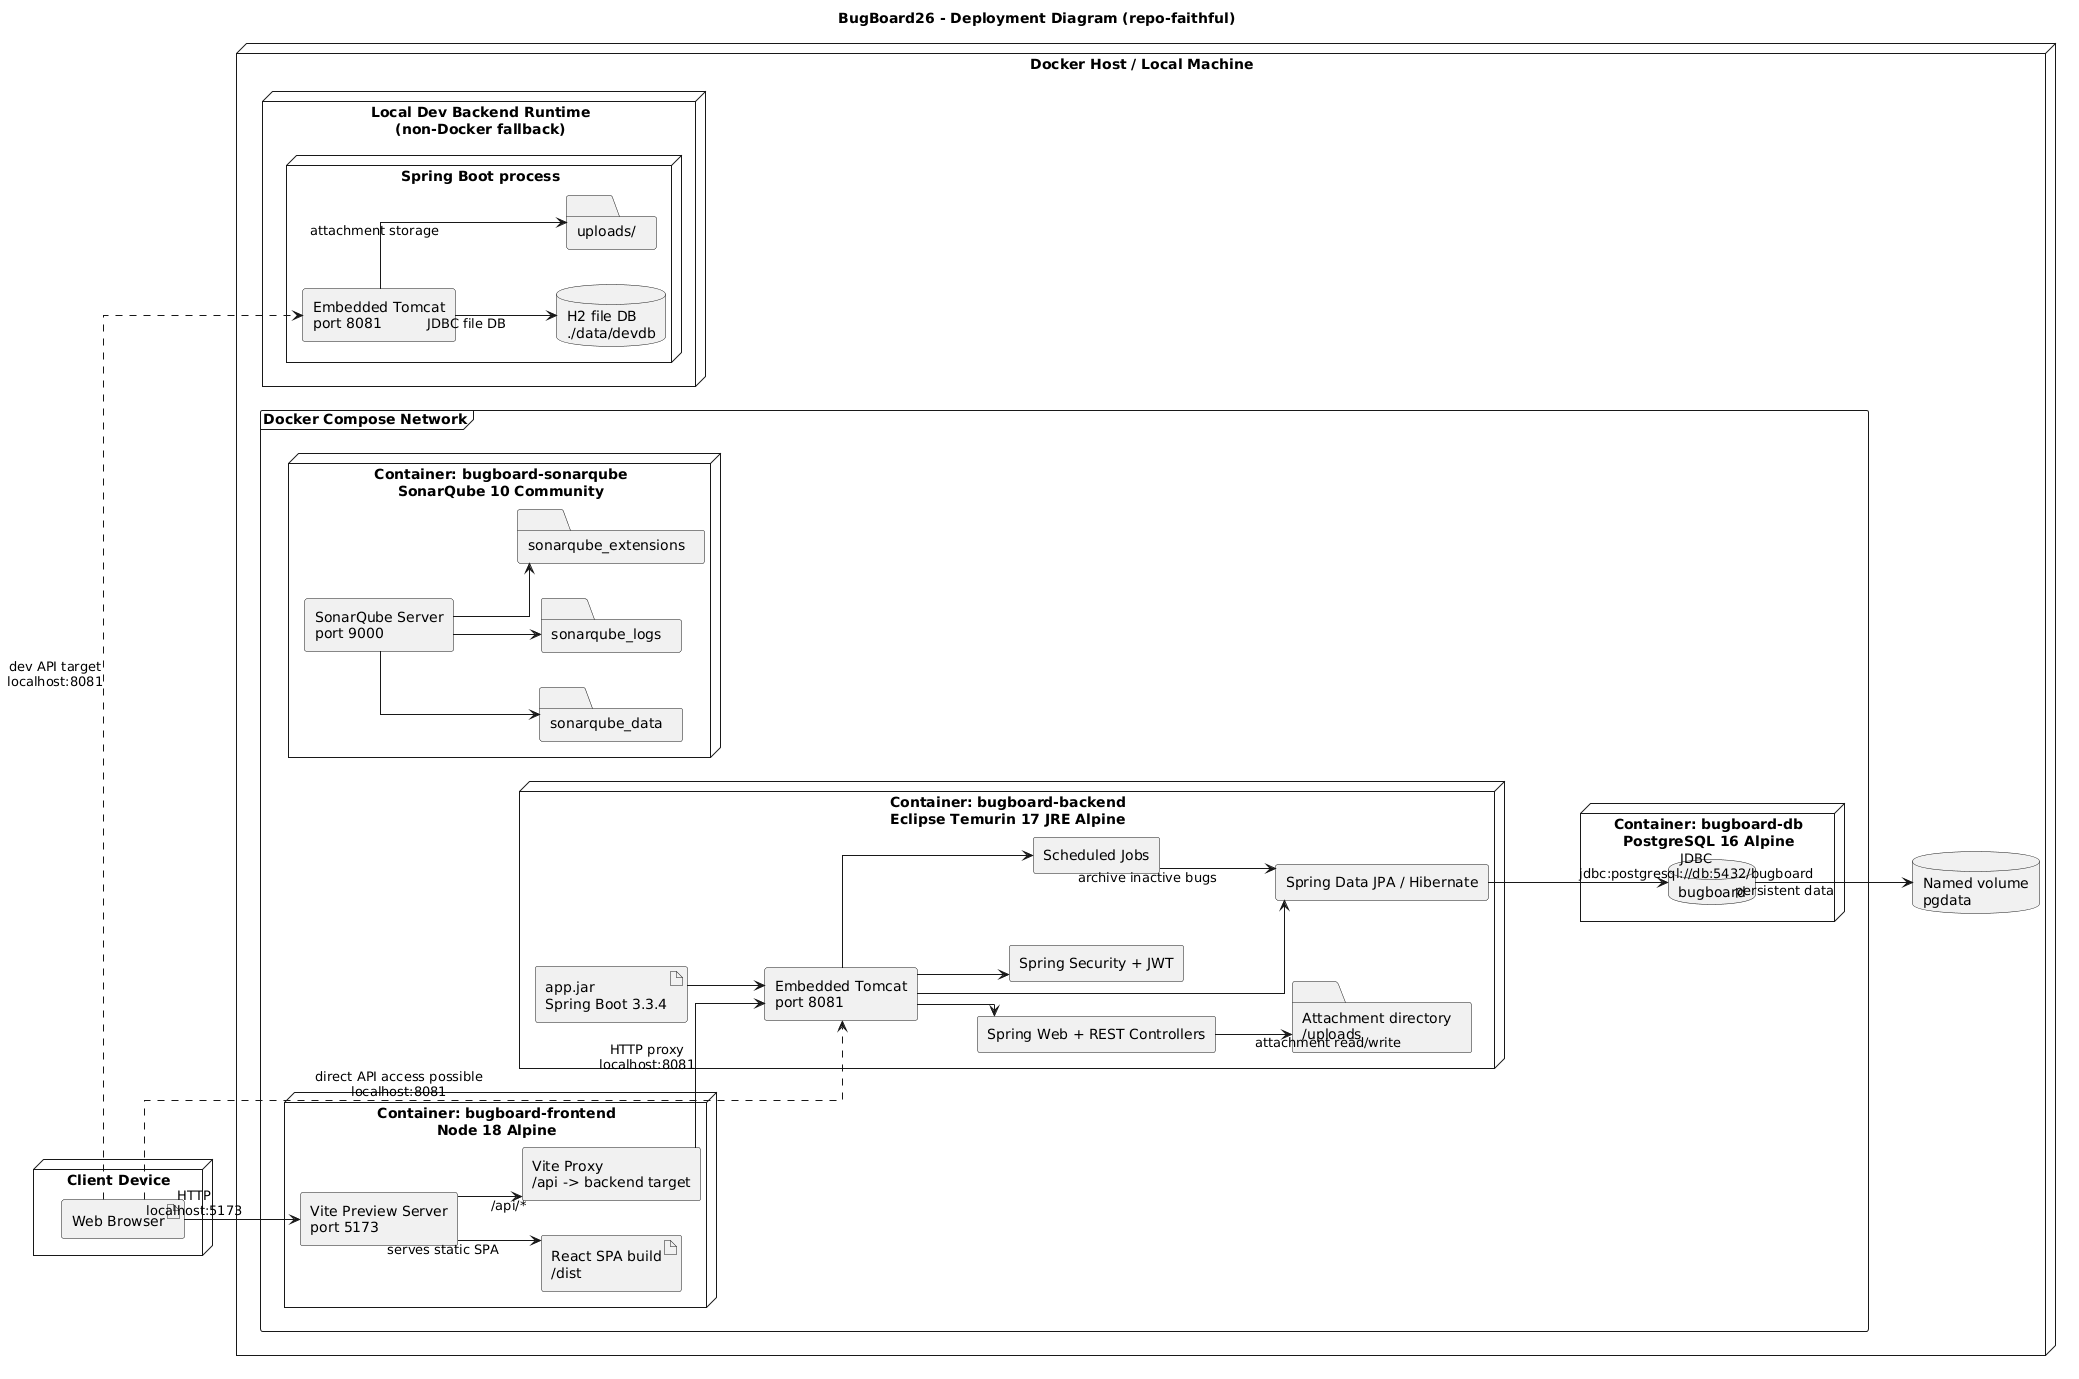
\includegraphics[width=\textwidth,height=0.82\textheight,keepaspectratio]{deployment_diagram_detailed.png}
\caption{Deployment Diagram dettagliato con ambiente Docker, fallback locale e volumi persistenti}
\end{figure}

\begin{figure}[H]
\centering
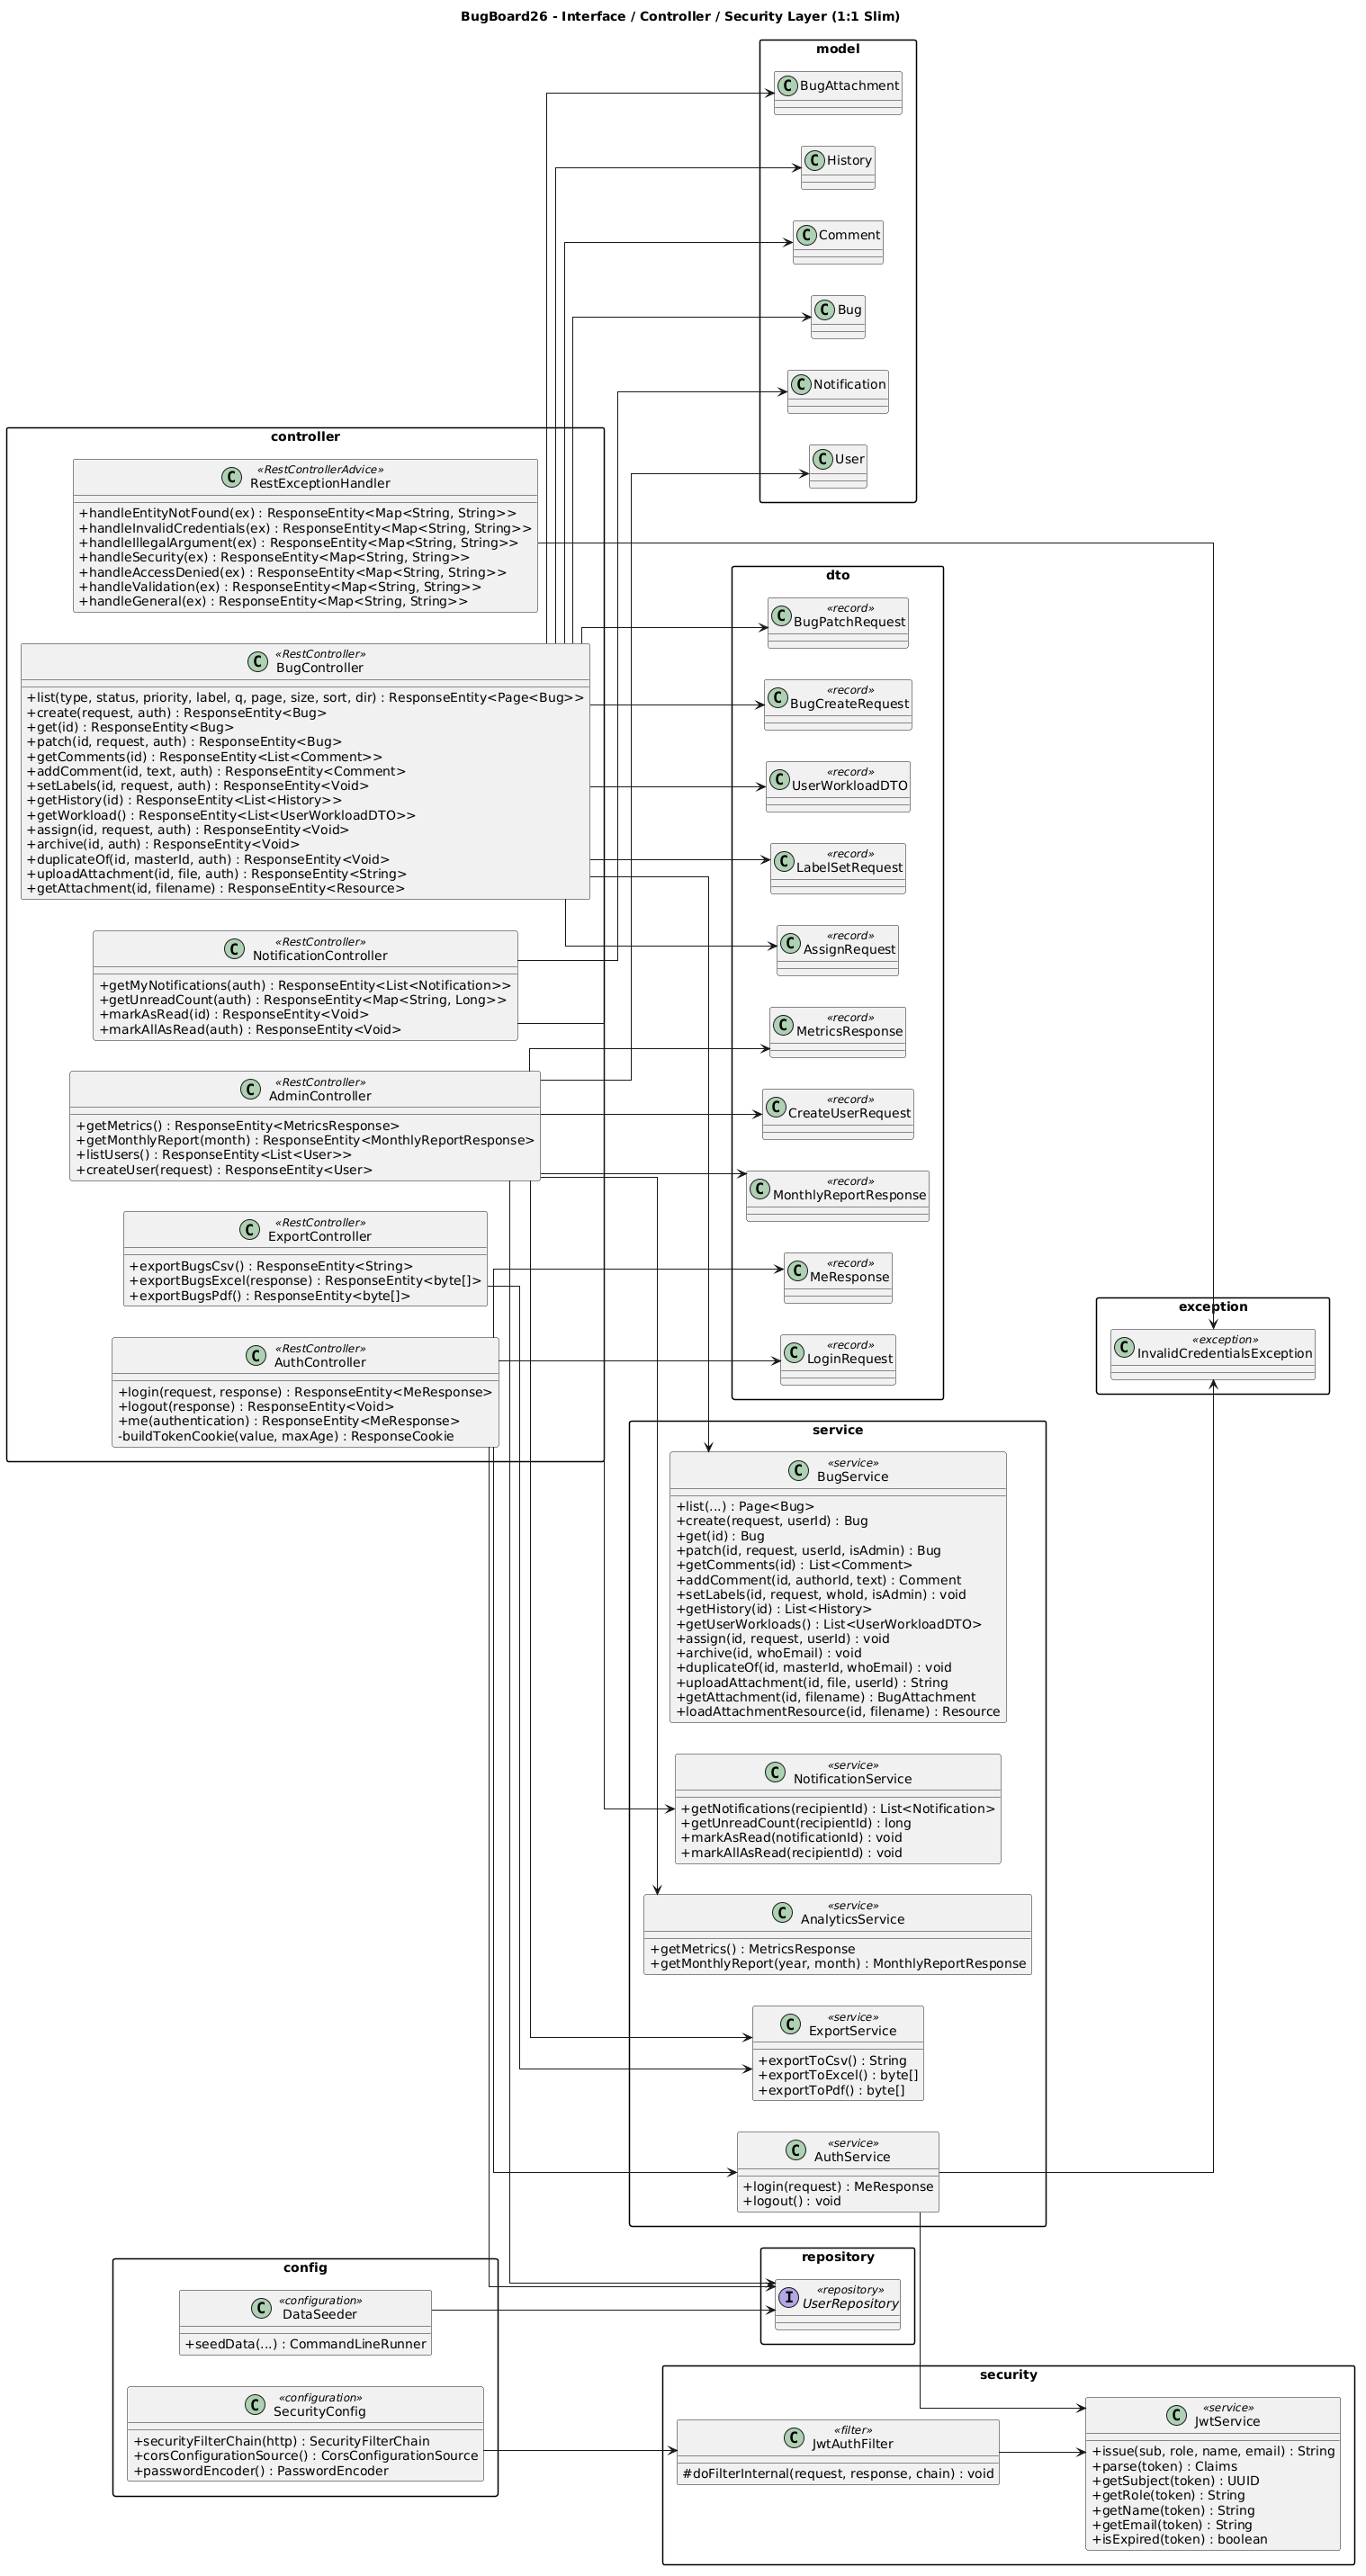
\includegraphics[width=0.82\textwidth,height=0.86\textheight,keepaspectratio]{interface_controller_security_layer.png}
\caption{Vista dettagliata del layer Interface / Controller / Security}
\end{figure}

\begin{figure}[H]
\centering
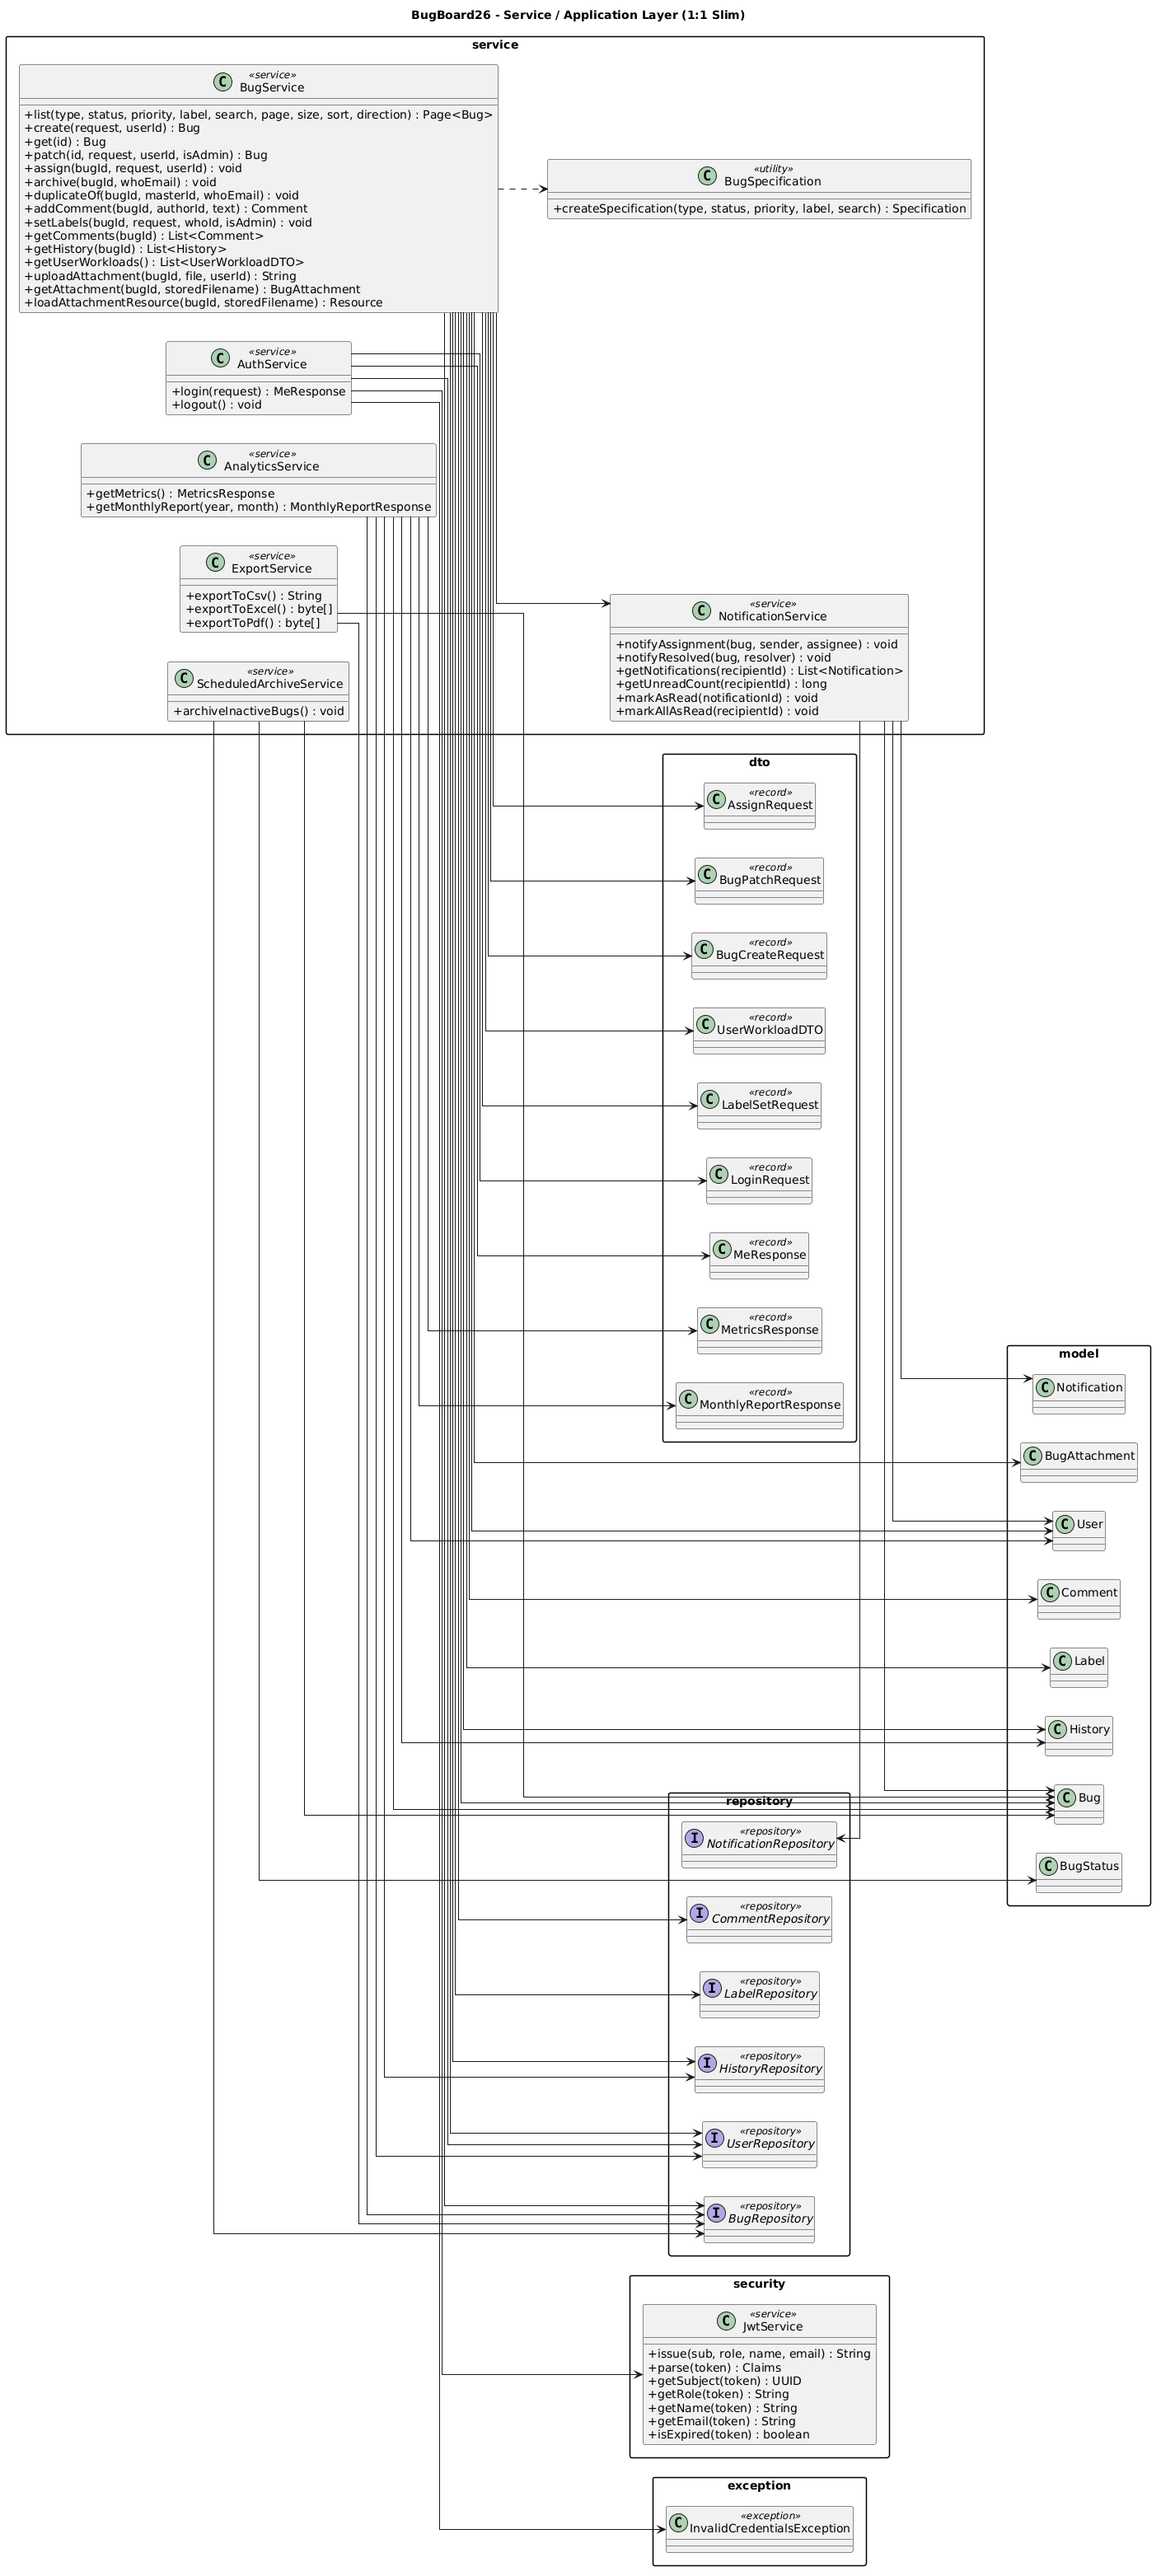
\includegraphics[width=0.82\textwidth,height=0.86\textheight,keepaspectratio]{service_application_layer.png}
\caption{Vista dettagliata del layer Service / Application}
\end{figure}

\subsection{Criteri di design adottati}

\begin{description}[style=nextline]
\item[\textbf{Separazione delle responsabilit\`a} (\emph{Separation of Concerns})] Ogni livello ha una responsabilit\`a ben definita: il frontend si occupa esclusivamente della presentazione e dell'interazione utente, il backend della logica di business e dell'autorizzazione, il database della persistenza. Questa separazione favorisce la manutenibilit\`a e la testabilit\`a.

\item[\textbf{Stateless Authentication}] L'autenticazione \`e gestita tramite token JWT, eliminando la necessit\`a di sessioni server-side. Ogni richiesta contiene il token necessario per l'identificazione, facilitando la scalabilit\`a orizzontale.

\item[\textbf{API-First Design}] Il backend espone un'API RESTful documentata tramite OpenAPI/Swagger (SpringDoc). Questo approccio consente lo sviluppo indipendente di frontend e backend, facilita l'integrazione con altri client e permette il testing automatico delle API.

\item[\textbf{Convention over Configuration}] L'utilizzo di Spring Boot riduce drasticamente la configurazione boilerplate grazie alle \emph{auto-configurations} e alle convenzioni del framework.

\item[\textbf{Containerizzazione}] L'intero stack \`e containerizzabile tramite Docker e orchestrabile con Docker Compose, garantendo riproducibilit\`a dell'ambiente e facilit\`a di deployment.
\end{description}

\subsection{Scelte tecnologiche}

\subsubsection{Frontend}

\begin{tabular}{|l|l|p{8cm}|}
\hline
\textbf{Tecnologia} & \textbf{Versione} & \textbf{Motivazione} \\
\hline
React & 18.x & Libreria UI component-based matura e con vasto ecosistema; facilita la creazione di SPA reattive. \\
\hline
TypeScript & 5.x & Tipizzazione statica che riduce i bug a runtime e migliora la manutenibilit\`a del codice. \\
\hline
Vite & 5.4.x & Build tool moderno, significativamente pi\`u veloce di Webpack grazie a ESBuild e HMR nativo. \\
\hline
Tailwind CSS & 3.x & Framework CSS utility-first che accelera lo sviluppo della UI e garantisce consistenza visiva. \\
\hline
Radix UI & -- & Componenti accessibili e non stilizzati (\emph{headless}), conformi a WAI-ARIA, personalizzabili con Tailwind. \\
\hline
React Query & 5.x & Infrastruttura condivisa per la gestione dello stato server-side; nell'implementazione corrente \`e predisposto tramite \texttt{QueryClientProvider} e integrato gradualmente accanto alle chiamate API manuali. \\
\hline
React Router & 6.30.x & Routing dichiarativo per SPA con supporto a route protette e navigazione client-side. \\
\hline
\end{tabular}

\subsubsection{Backend}

\begin{tabular}{|l|l|p{8cm}|}
\hline
\textbf{Tecnologia} & \textbf{Versione} & \textbf{Motivazione} \\
\hline
Java & 17 & Linguaggio robusto e type-safe, con record per DTO concisi e ottimo supporto nell'ecosistema Spring Boot. \\
\hline
Spring Boot & 3.3.4 & Framework enterprise standard per applicazioni Java; auto-configuration, starter dependencies, embedded server. \\
\hline
Spring Security & -- & Gestione completa di autenticazione e autorizzazione; integrazione nativa con JWT. \\
\hline
Spring Data JPA & -- & Astrazione ORM che elimina il codice boilerplate per l'accesso ai dati; supporto a Specification per query dinamiche. \\
\hline
H2 Database & -- & Database embedded per lo sviluppo locale; nessuna installazione richiesta, avvio immediato. \\
\hline
PostgreSQL & 16 & Database relazionale per produzione; robusto, conforme ACID, supporto nativo a UUID. \\
\hline
JJWT & 0.12.5 & Libreria per la creazione e validazione di token JWT; API fluente e sicura. \\
\hline
SpringDoc & 2.6.0 & Generazione automatica della documentazione OpenAPI 3.0 dalle annotazioni Spring. \\
\hline
Apache POI & 5.3.0 & Generazione di file Excel (.xlsx) per l'export dei dati bug. \\
\hline
PDFBox & 2.0.30 & Generazione di documenti PDF per l'export dell'elenco bug. \\
\hline
\end{tabular}

\subsubsection{Testing}

\begin{tabular}{|l|p{10cm}|}
\hline
\textbf{Tecnologia} & \textbf{Motivazione} \\
\hline
JUnit 5 & Framework di testing standard per Java; supporto a test parametrizzati, display names, extensions. \\
\hline
Mockito 5 & Libreria di mocking che consente l'isolamento delle dipendenze nei test di unit\`a. \\
\hline
AssertJ & Asserzioni fluenti che migliorano la leggibilit\`a dei test. \\
\hline
\end{tabular}

\subsubsection{DevOps e Deployment}

\begin{tabular}{|l|p{10cm}|}
\hline
\textbf{Tecnologia} & \textbf{Motivazione} \\
\hline
Docker & Containerizzazione per ambienti riproducibili; Dockerfile multi-stage per build ottimizzati. \\
\hline
Docker Compose & Orchestrazione dei servizi del sistema (database, backend, frontend e tooling di qualit\`a) con un solo comando. \\
\hline
Git / GitHub & Version control distribuito; collaborazione, code review, CI/CD integration. \\
\hline
Maven & Build automation per il backend; gestione dipendenze, lifecycle standardizzato. \\
\hline
npm & Package manager per il frontend; gestione dipendenze e script di build. \\
\hline
\end{tabular}

\subsection{Comunicazione tra i livelli}

La comunicazione tra frontend e backend avviene tramite API REST su HTTP/HTTPS:

\begin{itemize}
  \item \textbf{Formato dati}: JSON (Content-Type: \texttt{application/json})
  \item \textbf{Autenticazione}: Token JWT trasportato tramite cookie HttpOnly (\texttt{token}) oppure header \texttt{Authorization: Bearer <token>}
  \item \textbf{Proxy in sviluppo}: Vite espone il frontend su \texttt{localhost:8080} e redirige \texttt{/api/*} al backend configurato (default \texttt{localhost:18081}), evitando problemi CORS durante lo sviluppo
  \item \textbf{Endpoint principali}:
  \begin{itemize}
    \item \texttt{POST /api/auth/login} --- Autenticazione
    \item \texttt{GET /api/auth/me} --- Profilo dell'utente autenticato
    \item \texttt{GET/POST /api/bugs} --- Listing e creazione bug
    \item \texttt{PATCH /api/bugs/\{id\}} --- Modifica bug
    \item \texttt{POST /api/bugs/\{id\}/assign} --- Assegnazione (admin)
    \item \texttt{GET /api/notifications} --- Centro notifiche
    \item \texttt{GET /api/bugs/workload} --- Carico di lavoro utenti per suggerimento assegnatario
    \item \texttt{GET /api/admin/metrics} --- Metriche (admin)
    \item \texttt{GET /api/export/bugs.csv} --- Export CSV
    \item \texttt{GET /api/export/bugs.xlsx} --- Export Excel
    \item \texttt{GET /api/export/bugs.pdf} --- Export PDF
  \end{itemize}
\end{itemize}

\subsection{Sicurezza}

\begin{itemize}
  \item \textbf{Password}: hash BCrypt con salt automatico
  \item \textbf{CSRF}: disabilitato (architettura stateless con JWT)
  \item \textbf{CORS}: configurazione restrittiva con whitelist degli origin consentiti
  \item \textbf{Sessioni}: nessuna sessione server-side (\texttt{SessionCreationPolicy.STATELESS})
  \item \textbf{Autorizzazione}: controllo a livello di servizio basato sul ruolo dell'utente (ADMIN, USER, READONLY)
  \item \textbf{Cookie JWT}: attributi \texttt{HttpOnly} e \texttt{SameSite=Lax} per mitigare XSS e CSRF
\end{itemize}

% ==================== 10. DESIGN DEL SOFTWARE ====================
\section{Design del Software}

\subsection{Schema per la persistenza dati}

Il database relazionale \`e gestito tramite JPA/Hibernate con strategia \texttt{ddl-auto=update}. Di seguito lo schema entit\`a-relazione con tutte le tabelle, colonne e vincoli.

\subsubsection{Tabella \texttt{users}}

\begin{tabular}{|l|l|l|p{5cm}|}
\hline
\textbf{Colonna} & \textbf{Tipo} & \textbf{Vincoli} & \textbf{Note} \\
\hline
\texttt{id} & UUID & PK, AUTO & Identificativo univoco \\
\hline
\texttt{email} & VARCHAR & UNIQUE, NOT NULL & Indirizzo email \\
\hline
\texttt{password\_hash} & CHAR(60) & NOT NULL & Hash BCrypt \\
\hline
\texttt{name} & VARCHAR & NOT NULL & Nome visualizzato \\
\hline
\texttt{role} & VARCHAR & NOT NULL & Enum: ADMIN, USER, READONLY \\
\hline
\texttt{created\_at} & TIMESTAMP & & Data di registrazione \\
\hline
\end{tabular}

\subsubsection{Tabella \texttt{bugs}}

\begin{tabular}{|l|l|l|p{5cm}|}
\hline
\textbf{Colonna} & \textbf{Tipo} & \textbf{Vincoli} & \textbf{Note} \\
\hline
\texttt{id} & UUID & PK, AUTO & Identificativo univoco \\
\hline
\texttt{title} & VARCHAR & NOT NULL & Titolo del bug \\
\hline
\texttt{description} & TEXT & NOT NULL & Descrizione dettagliata \\
\hline
\texttt{type} & VARCHAR & NOT NULL & Enum: QUESTION, BUG, DOCUMENTATION, FEATURE \\
\hline
\texttt{status} & VARCHAR & & Enum: TODO, IN\_PROGRESS, RESOLVED, ARCHIVED \\
\hline
\texttt{priority} & VARCHAR & & Enum: LOW, MEDIUM, HIGH, URGENT \\
\hline
\texttt{archived} & BOOLEAN & default false & Flag di archiviazione \\
\hline
\texttt{created\_at} & TIMESTAMP & & Data di creazione \\
\hline
\texttt{updated\_at} & TIMESTAMP & & Data ultimo aggiornamento \\
\hline
\texttt{deadline} & TIMESTAMP & nullable & Scadenza opzionale \\
\hline
\texttt{duplicate\_of} & UUID & FK $\to$ bugs.id & Bug duplicato (self-ref) \\
\hline
\texttt{created\_by} & UUID & FK $\to$ users.id & Creatore \\
\hline
\texttt{assignee\_id} & UUID & FK $\to$ users.id & Assegnatario \\
\hline
\end{tabular}

\subsubsection{Tabella \texttt{comments}}

\begin{tabular}{|l|l|l|p{5cm}|}
\hline
\textbf{Colonna} & \textbf{Tipo} & \textbf{Vincoli} & \textbf{Note} \\
\hline
\texttt{id} & UUID & PK, AUTO & Identificativo univoco \\
\hline
\texttt{text} & TEXT & NOT NULL & Testo del commento \\
\hline
\texttt{bug\_id} & UUID & FK $\to$ bugs.id, NOT NULL & Bug associato \\
\hline
\texttt{author\_id} & UUID & FK $\to$ users.id, NOT NULL & Autore \\
\hline
\texttt{created\_at} & TIMESTAMP & & Data di creazione \\
\hline
\end{tabular}

\subsubsection{Tabella \texttt{history}}

\begin{tabular}{|l|l|l|p{5cm}|}
\hline
\textbf{Colonna} & \textbf{Tipo} & \textbf{Vincoli} & \textbf{Note} \\
\hline
\texttt{id} & UUID & PK, AUTO & Identificativo univoco \\
\hline
\texttt{bug\_id} & UUID & FK $\to$ bugs.id, NOT NULL & Bug associato \\
\hline
\texttt{who\_id} & UUID & FK $\to$ users.id, NOT NULL & Utente esecutore \\
\hline
\texttt{action} & VARCHAR & NOT NULL & Enum: CREATE, UPDATE, ASSIGN, COMMENT, ARCHIVE, DUPLICATE, LABELS\_SET, ATTACHMENT\_UPLOADED \\
\hline
\texttt{details} & TEXT & nullable & Dettagli del cambiamento \\
\hline
\texttt{created\_at} & TIMESTAMP & & Timestamp dell'azione \\
\hline
\end{tabular}

\subsubsection{Tabella \texttt{labels}}

\begin{tabular}{|l|l|l|p{5cm}|}
\hline
\textbf{Colonna} & \textbf{Tipo} & \textbf{Vincoli} & \textbf{Note} \\
\hline
\texttt{id} & UUID & PK, AUTO & Identificativo univoco \\
\hline
\texttt{name} & VARCHAR & UNIQUE, NOT NULL & Nome della label \\
\hline
\texttt{created\_at} & TIMESTAMP & & Data di creazione \\
\hline
\end{tabular}

\subsubsection{Tabella di join \texttt{bug\_labels}}

\begin{tabular}{|l|l|l|p{5cm}|}
\hline
\textbf{Colonna} & \textbf{Tipo} & \textbf{Vincoli} & \textbf{Note} \\
\hline
\texttt{bug\_id} & UUID & FK $\to$ bugs.id & Relazione molti-a-molti Bug $\leftrightarrow$ Label \\
\hline
\texttt{label\_id} & UUID & FK $\to$ labels.id & \\
\hline
\end{tabular}

\subsubsection{Tabella \texttt{notifications}}

\begin{tabular}{|l|l|l|p{5cm}|}
\hline
\textbf{Colonna} & \textbf{Tipo} & \textbf{Vincoli} & \textbf{Note} \\
\hline
\texttt{id} & UUID & PK, AUTO & Identificativo univoco \\
\hline
\texttt{recipient\_id} & UUID & FK $\to$ users.id, NOT NULL & Destinatario della notifica \\
\hline
\texttt{sender\_id} & UUID & FK $\to$ users.id & Utente che ha generato l'evento, se presente \\
\hline
\texttt{bug\_id} & UUID & FK $\to$ bugs.id, NOT NULL & Bug correlato alla notifica \\
\hline
\texttt{message} & TEXT & NOT NULL & Messaggio mostrato nel centro notifiche \\
\hline
\texttt{is\_read} & BOOLEAN & default false & Stato di lettura \\
\hline
\texttt{created\_at} & TIMESTAMP & & Data di creazione \\
\hline
\end{tabular}

\subsubsection{Collection table \texttt{bug\_attachments}}

\begin{tabular}{|l|l|l|p{5cm}|}
\hline
\textbf{Colonna} & \textbf{Tipo} & \textbf{Vincoli} & \textbf{Note} \\
\hline
\texttt{bug\_id} & UUID & FK $\to$ bugs.id, NOT NULL & Bug proprietario dell'allegato \\
\hline
\texttt{stored\_filename} & VARCHAR & NOT NULL & Nome interno del file memorizzato \\
\hline
\texttt{original\_filename} & VARCHAR & NOT NULL & Nome originale del file caricato \\
\hline
\texttt{content\_type} & VARCHAR & NOT NULL & MIME type dell'allegato \\
\hline
\texttt{file\_size} & BIGINT & NOT NULL & Dimensione in byte \\
\hline
\texttt{uploaded\_at} & TIMESTAMP & NOT NULL & Data di caricamento \\
\hline
\end{tabular}

\subsubsection{Diagramma E-R semplificato}

Il diagramma E-R semplificato aggiornato, coerente con l'implementazione corrente del backend, \`e riportato in Figura~\ref{fig:er_diagram}.

\begin{figure}[H]
\centering
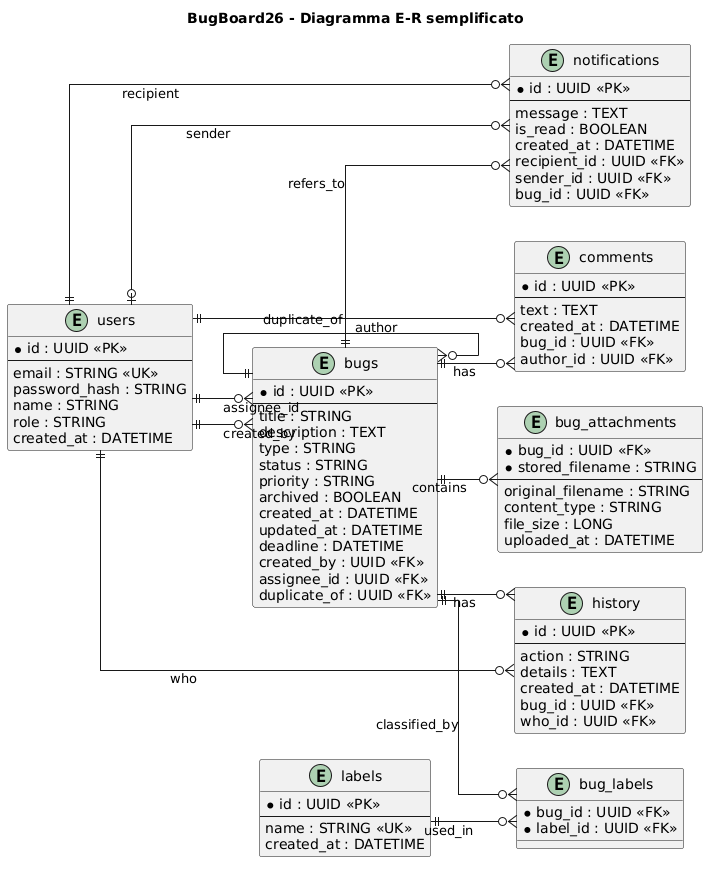
\includegraphics[width=0.95\textwidth]{diagramma_er_semplificato.png}
\caption{Diagramma E-R semplificato del database di BugBoard26}
\label{fig:er_diagram}
\end{figure}

\subsubsection{Diagramma di persistenza dettagliato}

Per affiancare la vista E-R semplificata, in Figura~\ref{fig:persistence_detailed} \`e riportata anche una rappresentazione UML pi\`u dettagliata del layer di persistenza e dominio, utile a evidenziare repository, entit\`a, enumerazioni e associazioni principali in modo pi\`u vicino al codice.

\begin{figure}[H]
\centering
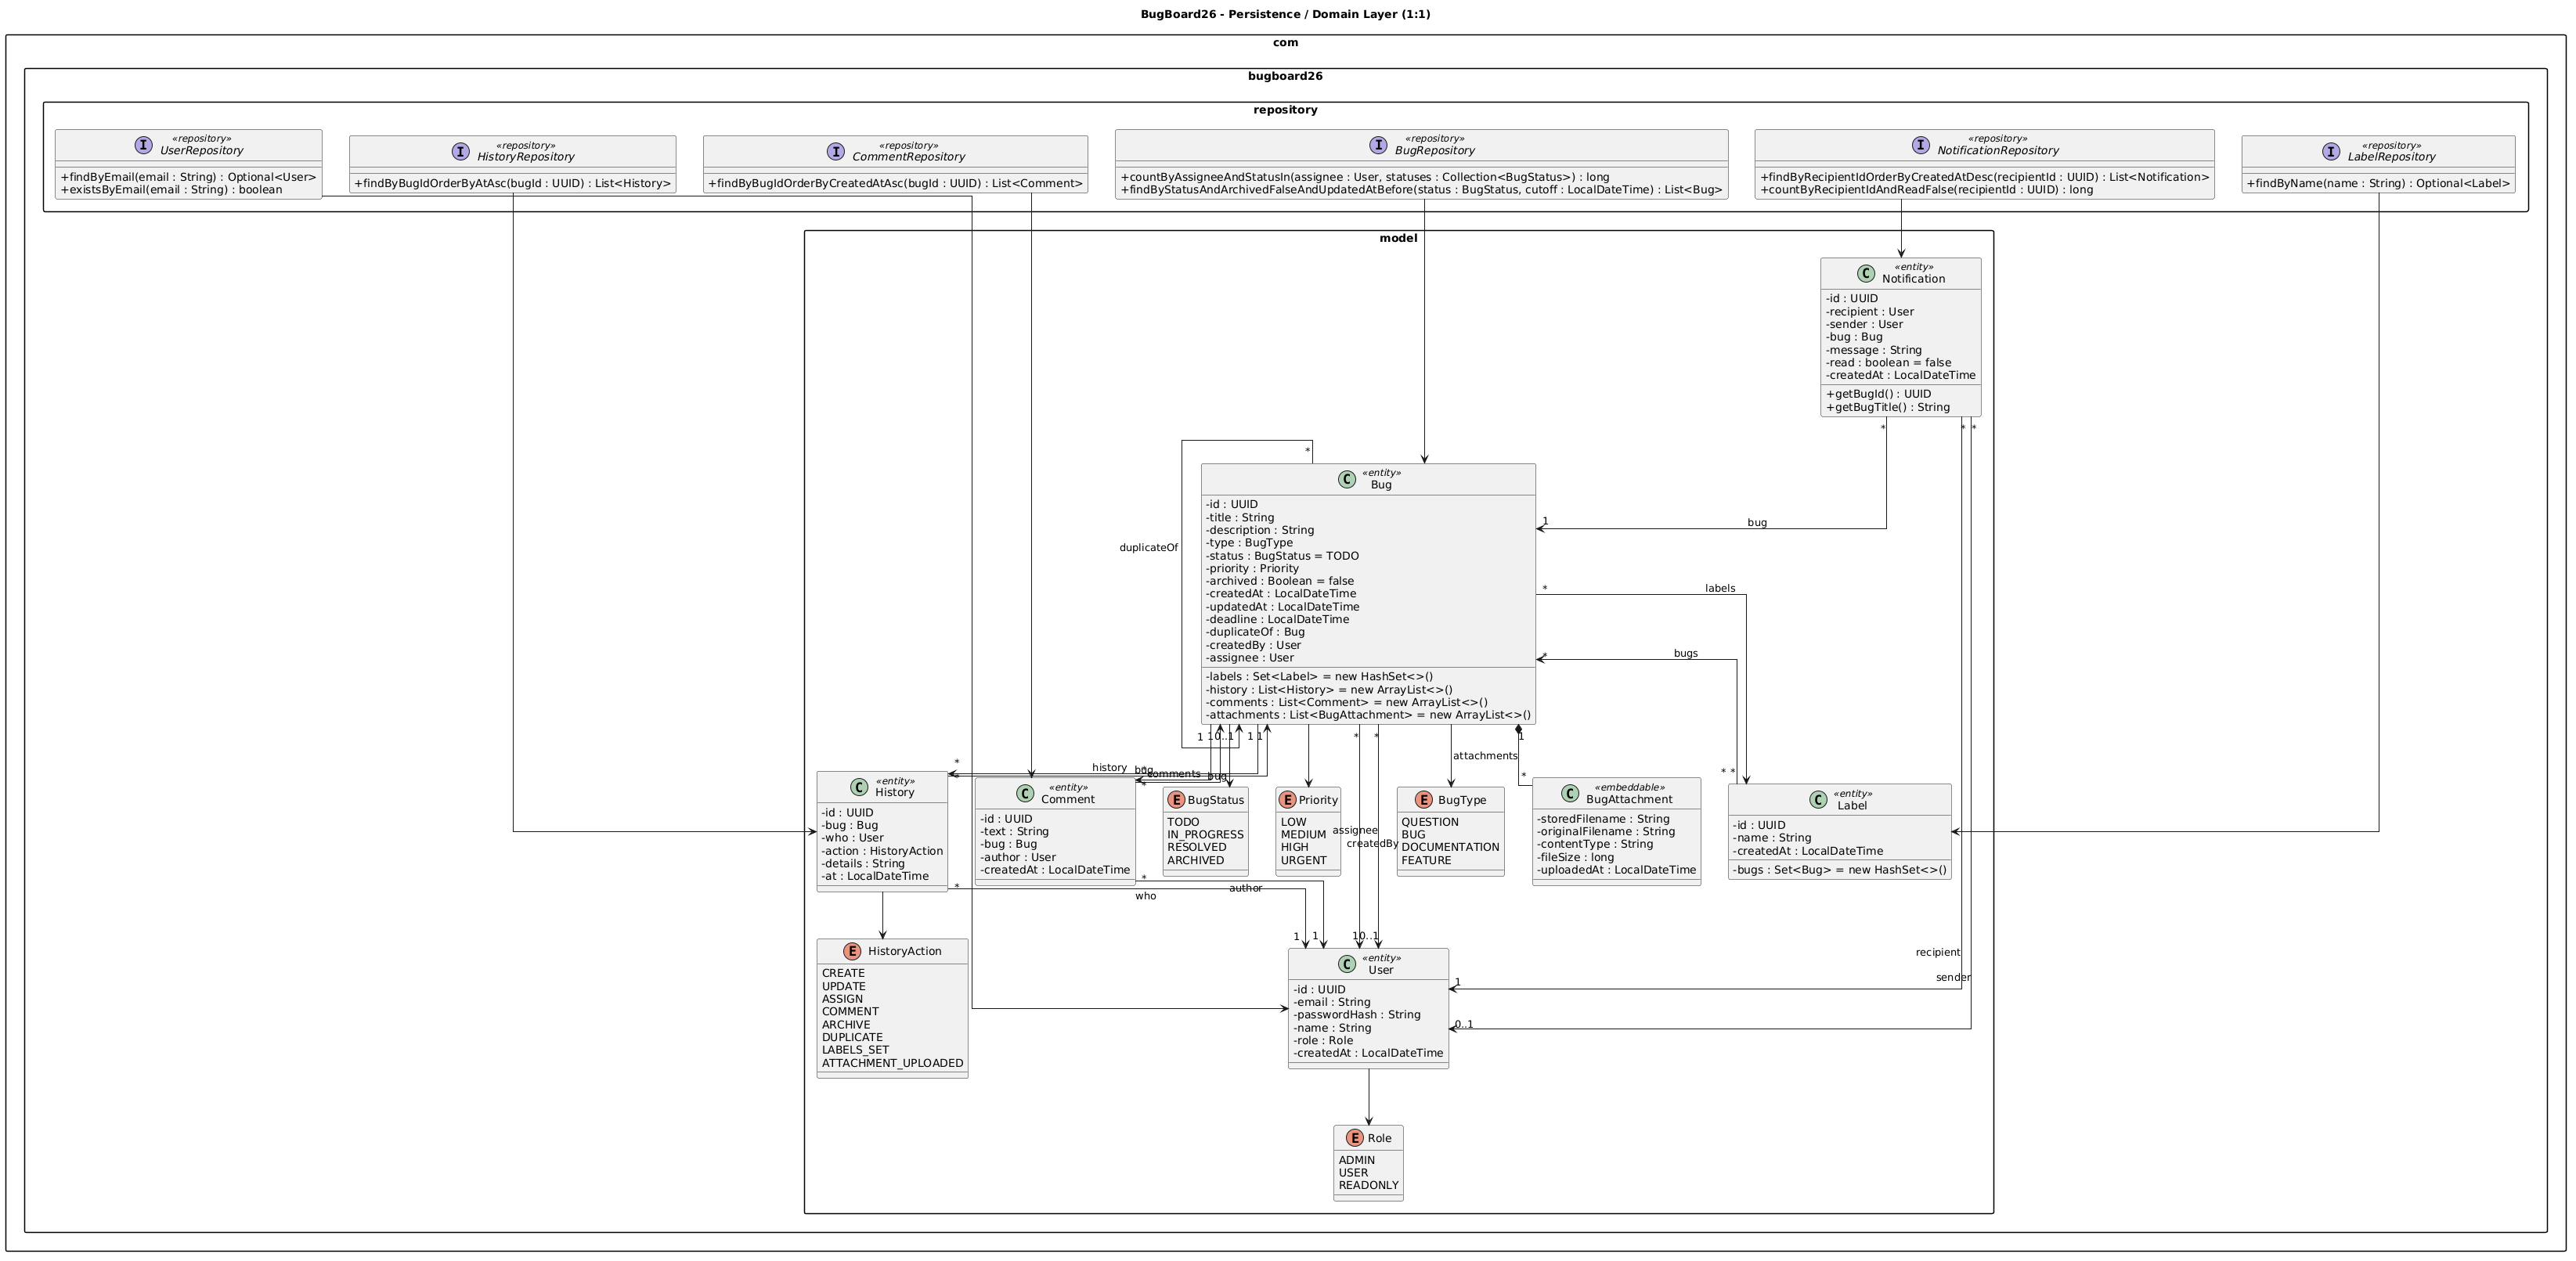
\includegraphics[width=\textwidth,height=0.82\textheight,keepaspectratio]{persistence_domain_detailed.png}
\caption{Diagramma UML dettagliato del layer di persistenza e dominio}
\label{fig:persistence_detailed}
\end{figure}

\subsection{Diagramma delle classi di design}

I diagrammi UML di analisi e design sono stati modellati tramite un \textbf{CASE tool} dedicato, nello specifico \textbf{StarUML}, e successivamente esportati e rifiniti per l'inclusione nella documentazione finale. Il diagramma delle classi di design \`e organizzato secondo il pattern architetturale \textbf{layered architecture} con i seguenti package:

\begin{description}[style=nextline]
\item[\texttt{model}] Entit\`a JPA che mappano le tabelle del database: \texttt{User}, \texttt{Bug}, \texttt{Comment}, \texttt{History}, \texttt{Label}, \texttt{Notification}, \texttt{BugAttachment} e le enumerazioni \texttt{Role}, \texttt{BugType}, \texttt{BugStatus}, \texttt{Priority}, \texttt{HistoryAction}.

\item[\texttt{repository}] Interfacce Spring Data JPA che estendono \texttt{JpaRepository<T, UUID>}: \texttt{UserRepository}, \texttt{BugRepository} (+ \texttt{JpaSpecificationExecutor}), \texttt{CommentRepository}, \texttt{LabelRepository}, \texttt{HistoryRepository}, \texttt{NotificationRepository}.

\item[\texttt{service}] Classi di business logic: \texttt{BugService}, \texttt{AuthService}, \texttt{AnalyticsService}, \texttt{ExportService}, \texttt{NotificationService}, \texttt{ScheduledArchiveService}, oltre a \texttt{BugSpecification} per la costruzione delle query dinamiche.

\item[\texttt{dto}] Record Java per i dati di trasferimento: \texttt{BugCreateRequest}, \texttt{BugPatchRequest}, \texttt{AssignRequest}, \texttt{LabelSetRequest}, \texttt{LoginRequest}, \texttt{CreateUserRequest}, \texttt{MeResponse}, \texttt{MetricsResponse}, \texttt{MonthlyReportResponse}, \texttt{MonthlyUserReportResponse}, \texttt{UserWorkloadDTO}.

\item[\texttt{controller}] Controller REST: \texttt{BugController} (\texttt{/api/bugs}), \texttt{AuthController} (\texttt{/api/auth}), \texttt{AdminController} (\texttt{/api/admin}), \texttt{NotificationController} (\texttt{/api/notifications}), \texttt{ExportController} (\texttt{/api/export}) e \texttt{RestExceptionHandler} per la gestione centralizzata degli errori HTTP.

\item[\texttt{security}] Infrastruttura di sicurezza: \texttt{JwtService} (generazione/validazione token), \texttt{JwtAuthFilter} (filtro per estrarre e verificare il JWT).

\item[\texttt{config}] Configurazione dell'applicazione: \texttt{SecurityConfig} (CORS, CSRF, filter chain), \texttt{DataSeeder} (dati iniziali per lo sviluppo).

\item[\texttt{exception}] Eccezioni applicative dedicate, ad esempio \texttt{InvalidCredentialsException}, usate per segnalare errori di dominio in modo esplicito.
\end{description}

Il diagramma delle classi di design aggiornato in coerenza con l'implementazione corrente è riportato in Figura~\ref{fig:class_diagram}.

\begin{figure}[H]
\centering
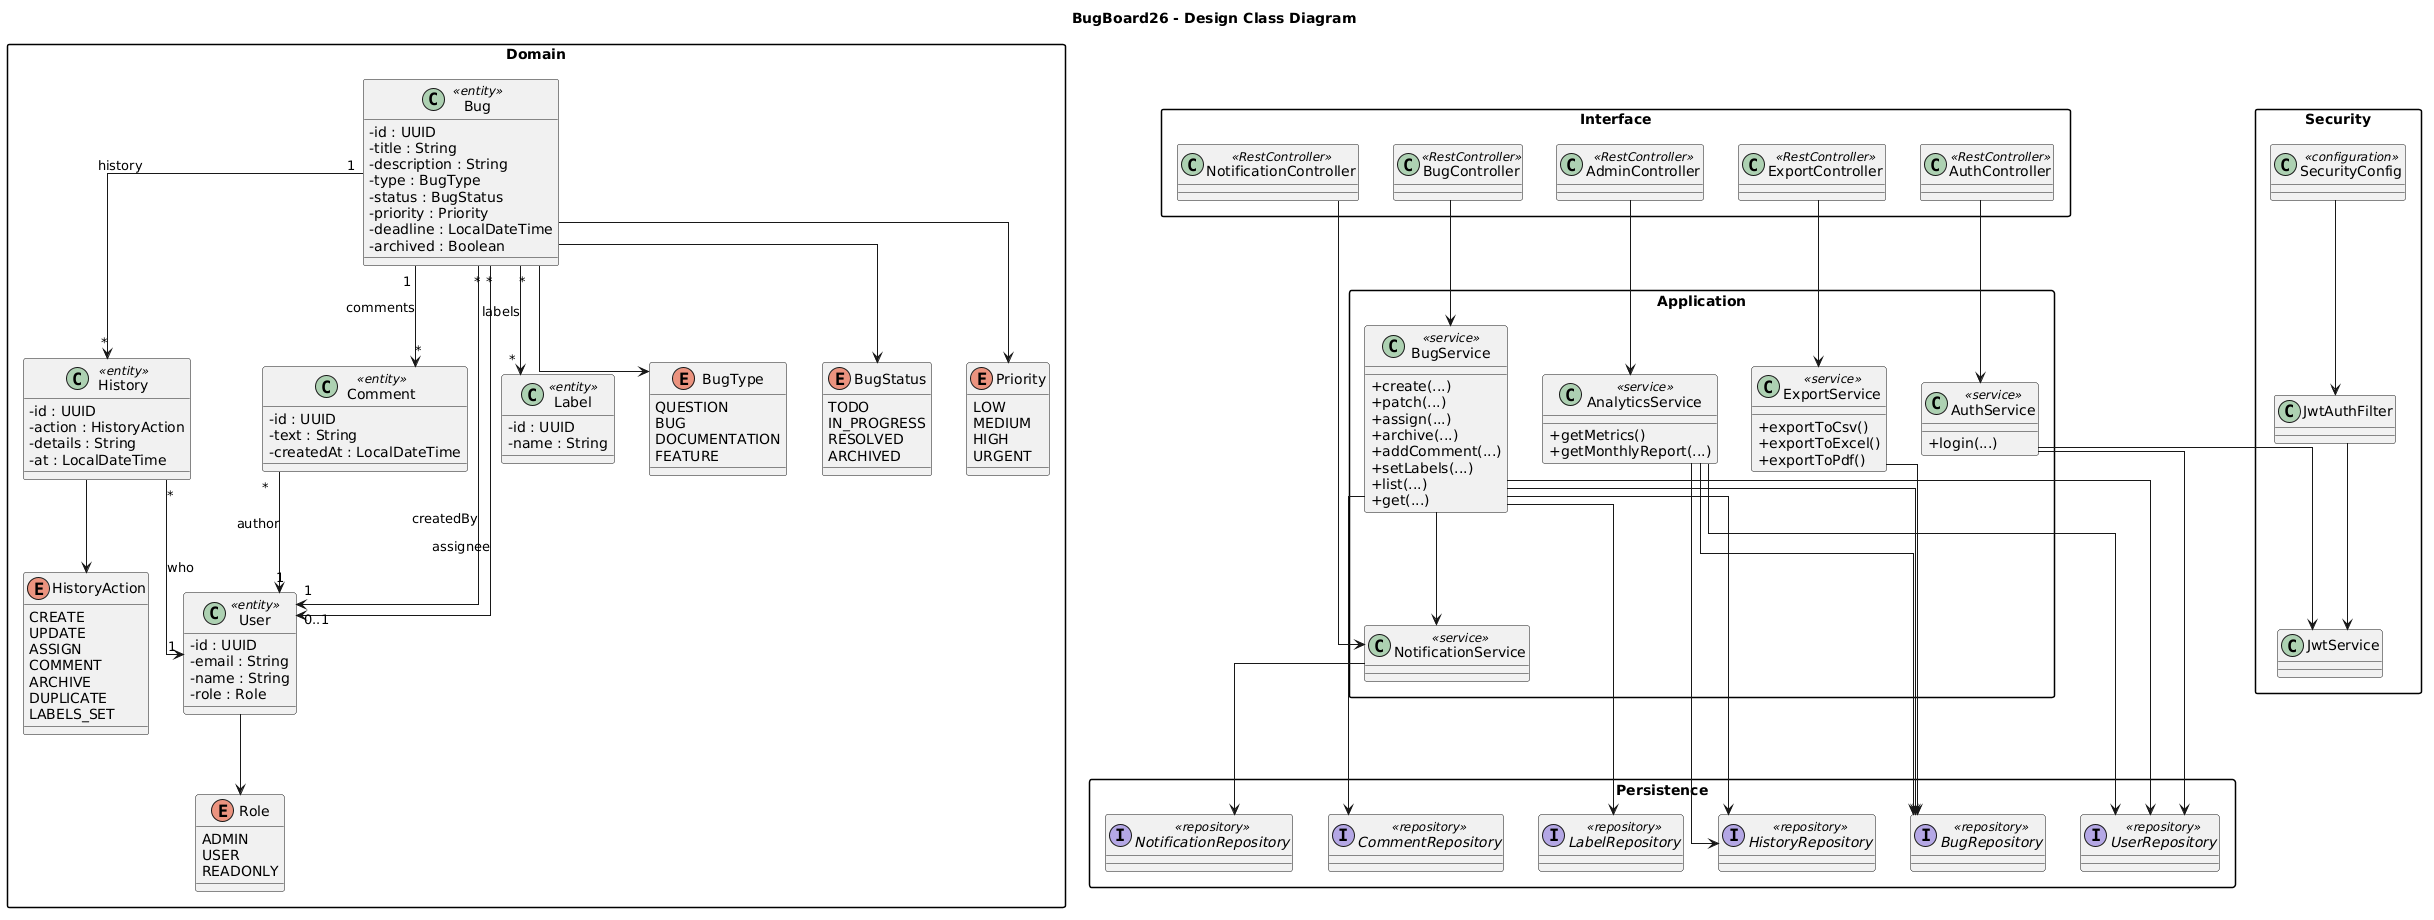
\includegraphics[width=\textwidth]{class_diagram.png}
\caption{Diagramma delle classi di design --- BugBoard26}
\label{fig:class_diagram}
\end{figure}

\subsection{Diagramma comportamentale --- Sequence Diagram}

Il sequence diagram in Figura~\ref{fig:sequence_diagram} illustra il flusso completo dell'operazione di \textbf{creazione di un nuovo bug}, dalla compilazione del form nell'interfaccia utente fino alla persistenza nel database. Questo caso d'uso \`e stato scelto in quanto coinvolge tutti i layer architetturali e presenta logica condizionale non banale (gestione labels, validazione utente).

\begin{figure}[H]
\centering
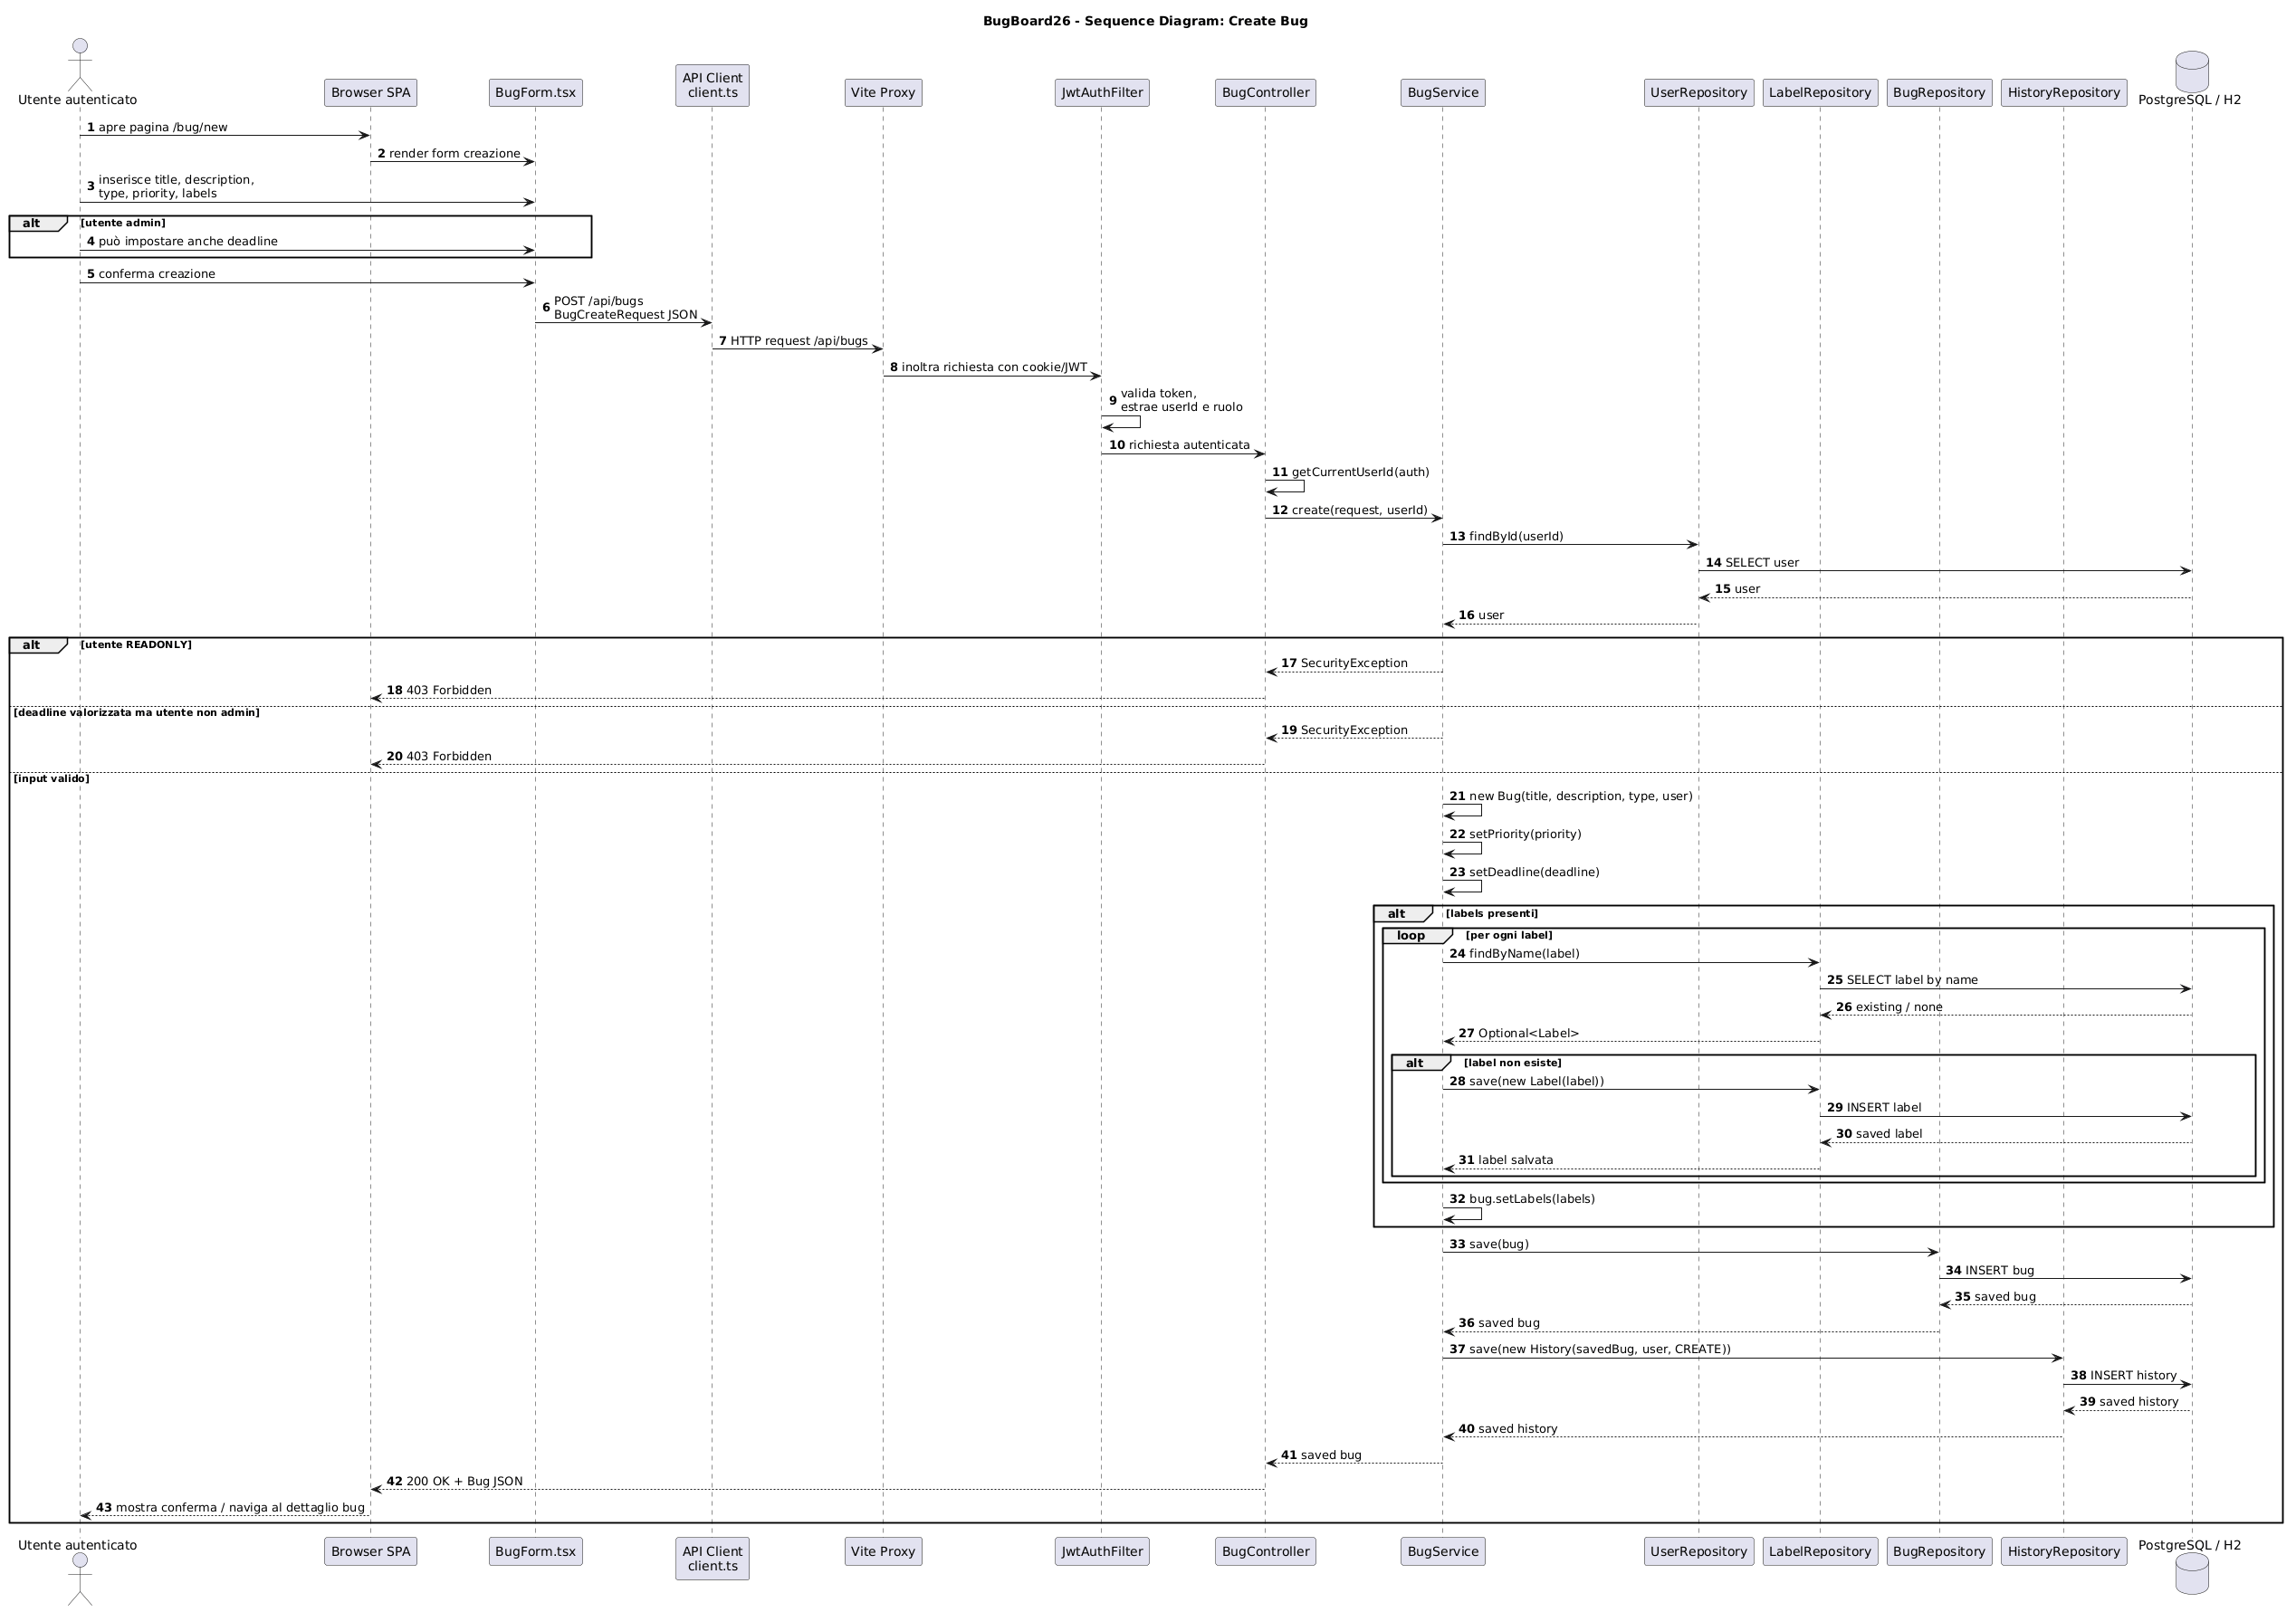
\includegraphics[width=\textwidth]{sequence_create_bug.png}
\caption{Sequence Diagram --- Creazione di un bug}
\label{fig:sequence_diagram}
\end{figure}

Per completezza \`e stato incluso anche un secondo sequence diagram relativo all'assegnazione di un bug, con evidenza esplicita del controllo ruolo amministratore, della scelta dell'assegnatario e della generazione della notifica.

\begin{figure}[H]
\centering
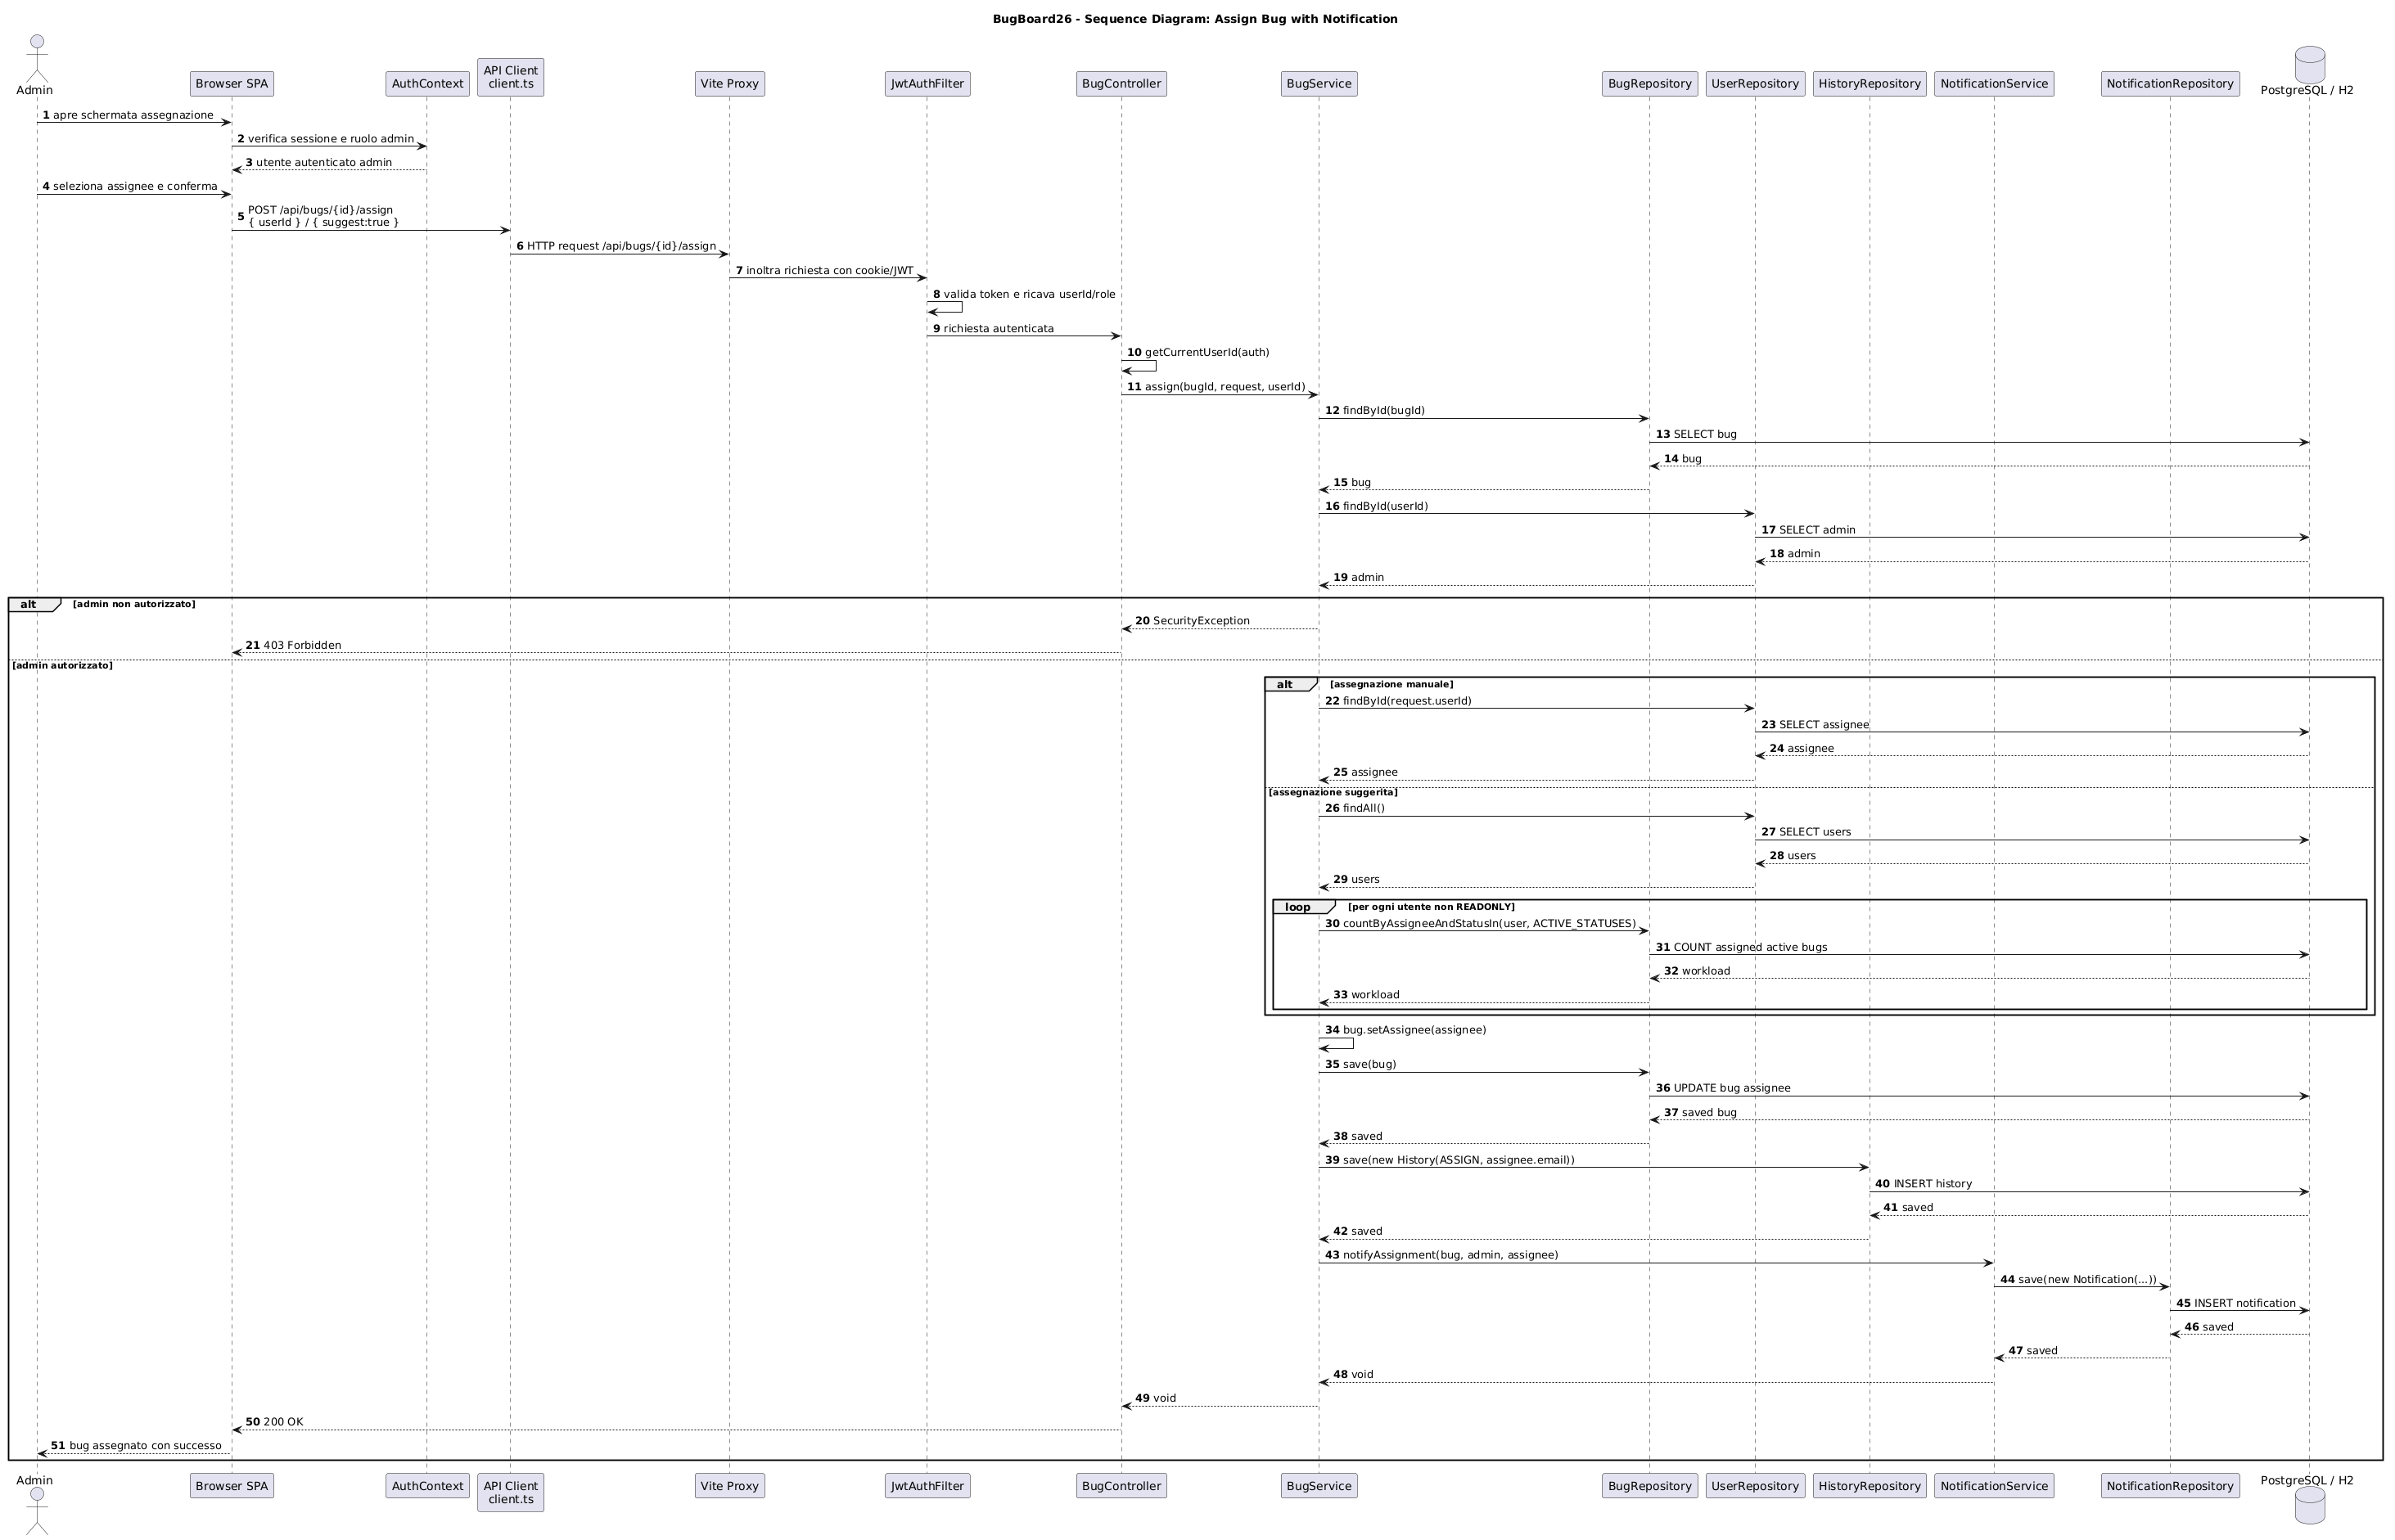
\includegraphics[width=\textwidth,height=0.82\textheight,keepaspectratio]{sequence_assign_bug.png}
\caption{Sequence Diagram --- Assegnazione di un bug con notifica}
\label{fig:sequence_assign}
\end{figure}

\subsection{Scelte di software design}

\subsubsection{Pattern Repository}
Ogni entit\`a dispone di un'interfaccia repository dedicata che estende \texttt{JpaRepository}. Questo pattern separa la logica di accesso ai dati dalla logica di business, favorendo la testabilit\`a tramite mock objects.

\texttt{BugRepository} estende anche \texttt{JpaSpecificationExecutor}, consentendo la costruzione di query dinamiche (filtri per tipo, stato, priorit\`a, label, ricerca testuale) senza codice SQL custom.

\subsubsection{Pattern Service Layer}
La logica di business \`e concentrata nei servizi (\texttt{BugService}, \texttt{AuthService}), che orchestrano le operazioni tra pi\`u repository. I controller sono \emph{thin}: delegano immediatamente ai servizi senza contenere logica di business.

\subsubsection{Record Java per i DTO}
I DTO sono implementati come \texttt{record} Java, che garantiscono immutabilit\`a, auto-generazione di \texttt{equals}/\texttt{hashCode}/\texttt{toString}, e riduzione del codice boilerplate. Le annotazioni di validazione (\texttt{@NotBlank}, \texttt{@NotNull}, \texttt{@NotEmpty}) sono applicate direttamente sui componenti del record.

\subsubsection{Specification Pattern per le query}
La classe \texttt{BugSpecification} implementa il pattern Specification di Spring Data, componendo predicati JPA Criteria in modo dichiarativo. I filtri (tipo, stato, priorit\`a, label, ricerca full-text su titolo e descrizione) possono essere combinati liberamente dal frontend.

\subsubsection{Audit Trail tramite History}
Ogni operazione significativa (creazione, modifica, assegnazione, commento, archiviazione) genera automaticamente una entry nella tabella \texttt{history}, con riferimento all'utente, all'azione e ai dettagli della modifica. Questo garantisce tracciabilit\`a completa senza librerie esterne.

\subsubsection{Autenticazione stateless con JWT}
\texttt{JwtService} genera token firmati HMAC-SHA256 con claims personalizzati (ruolo, nome, email). \texttt{JwtAuthFilter} intercetta ogni richiesta, estrae il token da cookie o header, e popola il \texttt{SecurityContext} di Spring Security. Questo approccio elimina la necessit\`a di sessioni server-side e facilita la scalabilit\`a orizzontale.

\subsubsection{Gestione delle autorizzazioni}
Il controllo degli accessi \`e implementato a due livelli:
\begin{itemize}
  \item \textbf{Livello HTTP}: Spring Security filtra le richieste in base all'autenticazione (JWT valido).
  \item \textbf{Livello Service}: le regole di business (solo admin pu\`o assegnare; solo assegnatario o admin pu\`o cambiare stato) sono verificate nel servizio, lanciando \texttt{SecurityException} in caso di violazione.
\end{itemize}

\subsection{Evidenza dell'uso di strumenti di versioning}

Il codice sorgente del progetto \`e ospitato su un repository \textbf{GitHub} accessibile ai membri del team di sviluppo.

\begin{itemize}
  \item \textbf{Repository}: \url{https://github.com/alessandroilprogrammatore/BugBoard26}
  \item \textbf{Release}: la release ``Specifica dei requisiti'' \`e stata pubblicata il 19 ottobre 2025
  \item \textbf{Branching strategy}: sviluppo su branch feature, merge su \texttt{main} tramite pull request
  \item \textbf{Commit}: messaggi descrittivi che seguono il formato convenzionale (\texttt{feat:}, \texttt{fix:}, \texttt{docs:}, \texttt{test:})
  \item \textbf{Statistiche repository}: 86 commit complessivi e 3 contributor rilevati nella history Git
  \item \textbf{Contributors}: Alessandro Minopoli, Simoalvin (Simone Mollo), PorfirioTramontana
  \item \textbf{Frequenza dei commit}: attivit\`a distribuita tra ottobre 2025 e marzo 2026, con una chiara intensificazione nella fase finale del progetto
\end{itemize}

\begin{figure}[H]
\centering
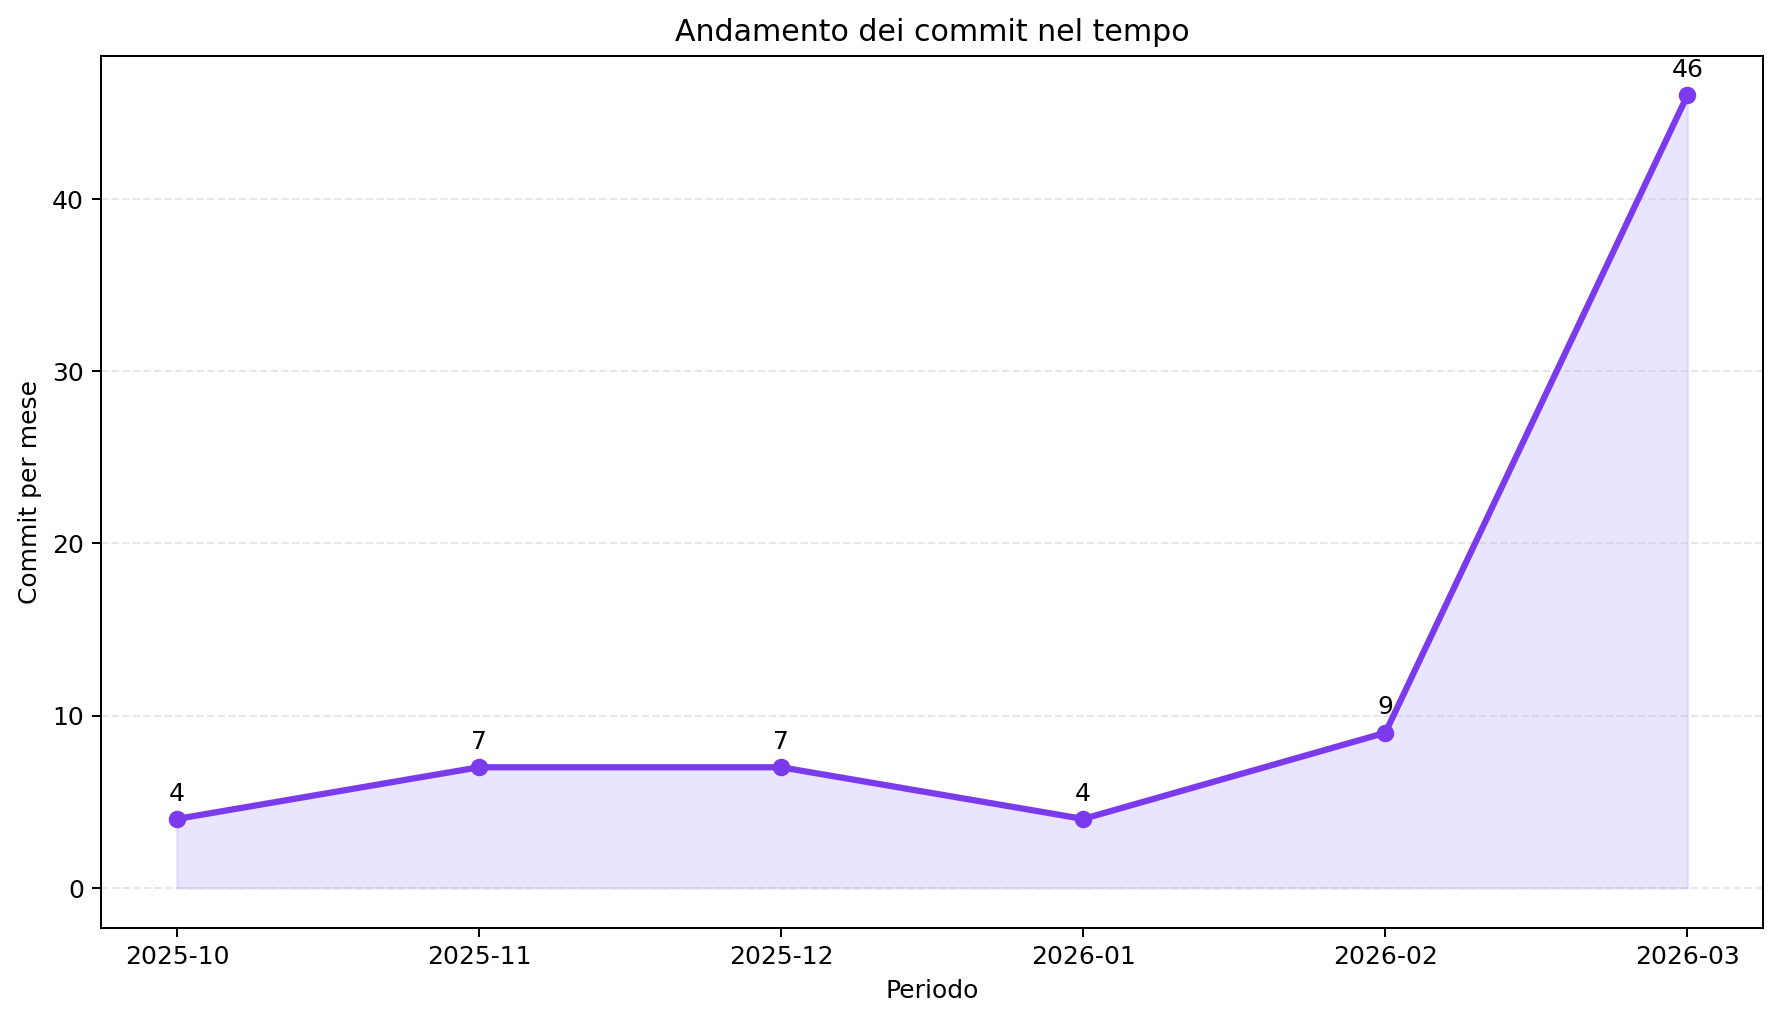
\includegraphics[width=0.82\textwidth]{git_commit_frequency_chart.png}
\caption{Andamento temporale dei commit nel repository}
\end{figure}

\begin{figure}[H]
\centering
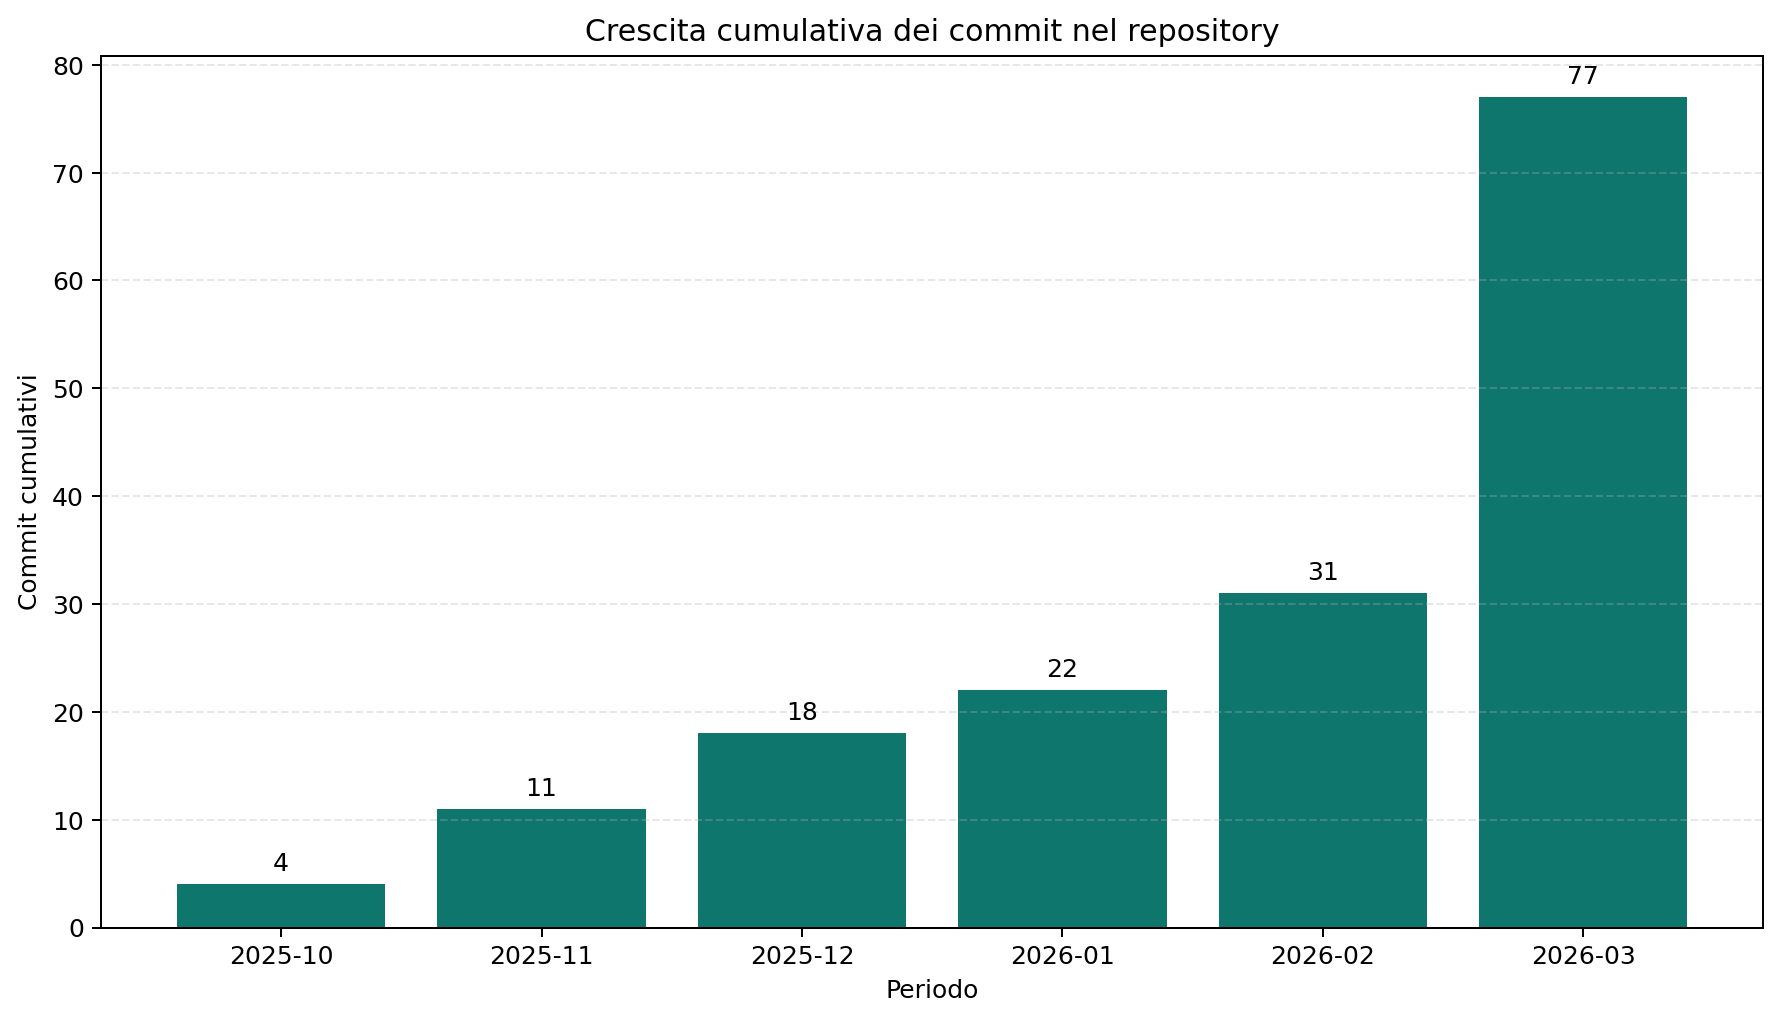
\includegraphics[width=0.82\textwidth]{git_commit_cumulative_chart.png}
\caption{Crescita cumulativa dei commit nel repository}
\end{figure}

% ==================== 11. TEST PLAN ====================
\section{Test Plan -- Gestione Bug}

\subsection{Obiettivo}
Il test plan descrive le attivit\`a di verifica previste per la funzionalit\`a \textbf{Gestione Bug} del sistema BugBoard26. L'obiettivo \`e validare che le operazioni di creazione, assegnazione e modifica di un bug rispettino i requisiti funzionali e le regole di autorizzazione definite nella specifica.

\subsection{Funzionalit\`a sotto test}
Le funzionalit\`a coperte dal piano sono quelle esposte dal servizio \texttt{BugService}:
\begin{enumerate}
  \item \textbf{Creazione di un bug} -- metodo \texttt{create(BugCreateRequest, UUID)}
  \item \textbf{Assegnazione di un bug} -- metodo \texttt{assign(UUID, AssignRequest, UUID)}
  \item \textbf{Modifica di un bug} -- metodo \texttt{patch(UUID, BugPatchRequest, UUID, boolean)}
\end{enumerate}

\subsection{Approccio di testing}
\begin{itemize}
  \item \textbf{Livello}: test di unit\`a (\emph{unit test}).
  \item \textbf{Tecnica}: \emph{black-box} (classi di equivalenza, valori limite) combinata con ispezione \emph{white-box} (copertura dei rami decisionali interni).
  \item \textbf{Framework}: JUnit 5 + Mockito 5 (via \texttt{spring-boot-starter-test}).
  \item \textbf{Isolamento}: le dipendenze esterne (\emph{repository} JPA e servizi ausiliari come \texttt{NotificationService}) sono sostituite da \emph{mock objects} iniettati con \texttt{@Mock} / \texttt{@InjectMocks}, garantendo che i test verifichino esclusivamente la logica di business senza accesso al database.
\end{itemize}

\subsection{Casi di test pianificati}

\subsubsection{\texttt{create(BugCreateRequest, UUID)}}

\begin{tabular}{|l|p{6.5cm}|p{6cm}|}
\hline
\textbf{ID} & \textbf{Scenario} & \textbf{Risultato atteso} \\
\hline
TC-C1 & Creazione con titolo, descrizione, tipo e priorit\`a validi & Bug salvato; history \texttt{CREATE} registrata \\
\hline
TC-C2 & UserId inesistente nel sistema & \texttt{EntityNotFoundException} \\
\hline
TC-C3 & Request con lista di label (alcune esistenti, altre nuove) & Bug con label associate; label inesistenti create automaticamente \\
\hline
\end{tabular}

\subsubsection{\texttt{assign(UUID, AssignRequest, UUID)}}

\begin{tabular}{|l|p{6.5cm}|p{6cm}|}
\hline
\textbf{ID} & \textbf{Scenario} & \textbf{Risultato atteso} \\
\hline
TC-A1 & Admin assegna bug a utente esistente & Assignee aggiornato; history \texttt{ASSIGN} registrata \\
\hline
TC-A2 & Utente non-admin tenta l'assegnazione & \texttt{SecurityException} \\
\hline
TC-A3 & BugId inesistente & \texttt{EntityNotFoundException} \\
\hline
\end{tabular}

\subsubsection{\texttt{patch(UUID, BugPatchRequest, UUID, boolean)}}

\begin{tabular}{|l|p{6.5cm}|p{6cm}|}
\hline
\textbf{ID} & \textbf{Scenario} & \textbf{Risultato atteso} \\
\hline
TC-P1 & Admin aggiorna titolo e priorit\`a & Campi aggiornati; history \texttt{UPDATE} registrata \\
\hline
TC-P2 & Non-admin tenta di cambiare stato di bug altrui & \texttt{SecurityException} \\
\hline
TC-P3 & Assegnatario modifica il proprio bug senza cambiare stato & Modifica applicata con successo \\
\hline
\end{tabular}

\subsection{Criteri di ingresso e uscita}

\textbf{Ingresso:} codice sorgente compilabile; dipendenze Maven risolte; ambiente Java 17+ configurato.

\textbf{Uscita:} la suite di unit test dedicata a \texttt{BugService} esegue 20 test con \texttt{BUILD SUCCESS}, 0 failures e 0 errors; copertura dei rami decisionali principali raggiunta.

\subsection{Ambiente di esecuzione}
\begin{itemize}
  \item \textbf{JDK}: Java 17 come baseline di progetto; esecuzione verificata anche su Eclipse Temurin 21.0.7 in ambiente containerizzato
  \item \textbf{Build tool}: Apache Maven con plugin Surefire 3.1.2
  \item \textbf{CI locale}: \texttt{mvn test} dalla directory \texttt{backend/}
\end{itemize}

% ==================== 12. STRATEGIE DI TESTING ====================
\section{Strategie di Testing}

Questa sezione documenta le strategie adottate per la progettazione dei test di unit\`a del servizio \texttt{BugService}, nucleo della logica di business dell'applicazione BugBoard26.

\subsection{Metodi testati}
Sono stati selezionati tre metodi non banali, ciascuno con almeno due parametri, come richiesto dalla specifica di progetto:

\begin{enumerate}
  \item \texttt{create(BugCreateRequest request, UUID userId)} -- 2 parametri
  \item \texttt{assign(UUID bugId, AssignRequest request, UUID userId)} -- 3 parametri
  \item \texttt{patch(UUID id, BugPatchRequest request, UUID userId, boolean isAdmin)} -- 4 parametri
\end{enumerate}

\subsection{Classi di equivalenza}

Per ciascun metodo sono state individuate le seguenti classi di equivalenza.

\subsubsection{\texttt{create(BugCreateRequest, UUID)}}

\begin{tabular}{|l|p{6cm}|l|l|}
\hline
\textbf{Classe} & \textbf{Condizione} & \textbf{Validit\`a} & \textbf{Test case} \\
\hline
EC-C1 & \texttt{userId} esistente; request con campi obbligatori validi, senza label & Valida & TC-C1 \\
\hline
EC-C2 & \texttt{userId} non presente nel database & Invalida & TC-C2 \\
\hline
EC-C3 & Request con lista di label non vuota (misto label esistenti e nuove) & Valida & TC-C3 \\
\hline
\end{tabular}

\subsubsection{\texttt{assign(UUID, AssignRequest, UUID)}}

\begin{tabular}{|l|p{6cm}|l|l|}
\hline
\textbf{Classe} & \textbf{Condizione} & \textbf{Validit\`a} & \textbf{Test case} \\
\hline
EC-A1 & Chiamante con ruolo \texttt{ADMIN}; bug e assegnatario esistenti & Valida & TC-A1 \\
\hline
EC-A2 & Chiamante con ruolo \texttt{USER} (non admin) & Invalida & TC-A2 \\
\hline
EC-A3 & \texttt{bugId} non presente nel database & Invalida & TC-A3 \\
\hline
\end{tabular}

\subsubsection{\texttt{patch(UUID, BugPatchRequest, UUID, boolean)}}

\begin{tabular}{|l|p{6cm}|l|l|}
\hline
\textbf{Classe} & \textbf{Condizione} & \textbf{Validit\`a} & \textbf{Test case} \\
\hline
EC-P1 & \texttt{isAdmin=true}; modifica di campi generici (titolo, priorit\`a) & Valida & TC-P1 \\
\hline
EC-P2 & \texttt{isAdmin=false}; cambio di \texttt{status} su bug assegnato ad altro utente & Invalida & TC-P2 \\
\hline
EC-P3 & \texttt{isAdmin=false}; modifica effettuata dall'assegnatario stesso (senza cambio di stato) & Valida & TC-P3 \\
\hline
\end{tabular}

% ==================== 12.X ANALISI DEI VALORI LIMITE (BVA) ====================
\subsection{Analisi dei Valori Limite (Boundary Value Analysis)}

L'analisi dei valori limite (BVA) complementa le classi di equivalenza concentrandosi sui confini delle condizioni di input, dove statisticamente si concentrano la maggior parte dei difetti.

\subsubsection{\texttt{create(BugCreateRequest, UUID)}}

\begin{tabular}{|l|p{5.5cm}|p{3cm}|p{4cm}|}
\hline
\textbf{ID} & \textbf{Valore limite} & \textbf{Tipo confine} & \textbf{Risultato atteso} \\
\hline
BV-C1 & Titolo con 1 carattere (minimo valido) & Limite inferiore & Bug creato con successo \\
\hline
BV-C2 & Titolo vuoto (0 caratteri) & Sotto il limite & Eccezione di validazione \\
\hline
BV-C3 & Titolo con 255 caratteri (massimo VARCHAR) & Limite superiore & Bug creato con successo \\
\hline
BV-C4 & Lista label vuota (\texttt{size = 0}) & Limite inferiore & Bug creato senza label \\
\hline
BV-C5 & Lista con 1 label (minimo non vuoto) & Appena sopra il limite & Bug creato con 1 label associata \\
\hline
BV-C6 & Descrizione con 1 carattere & Limite inferiore & Bug creato con successo \\
\hline
\end{tabular}

\subsubsection{\texttt{assign(UUID, AssignRequest, UUID)}}

\begin{tabular}{|l|p{5.5cm}|p{3cm}|p{4cm}|}
\hline
\textbf{ID} & \textbf{Valore limite} & \textbf{Tipo confine} & \textbf{Risultato atteso} \\
\hline
BV-A1 & Bug con assegnatario \texttt{null} (prima assegnazione) & Limite inferiore & Assignee impostato; history registrata \\
\hline
BV-A2 & Bug gi\`a assegnato allo stesso utente (riassegnazione identica) & Confine & Assegnazione eseguita (idempotente) \\
\hline
BV-A3 & Bug con assegnatario diverso (riassegnazione) & Sopra il limite & Assignee aggiornato; notifica al precedente \\
\hline
BV-A4 & \texttt{assigneeId} uguale a UUID nullo (\texttt{null}) & Confine invalido & Eccezione di validazione \\
\hline
\end{tabular}

\subsubsection{\texttt{patch(UUID, BugPatchRequest, UUID, boolean)}}

\begin{tabular}{|l|p{5.5cm}|p{3cm}|p{4cm}|}
\hline
\textbf{ID} & \textbf{Valore limite} & \textbf{Tipo confine} & \textbf{Risultato atteso} \\
\hline
BV-P1 & Request con tutti i campi \texttt{null} (nessuna modifica) & Limite inferiore & Bug invariato; nessuna history \\
\hline
BV-P2 & Request con un solo campo non \texttt{null} (modifica minima) & Appena sopra il limite & Solo quel campo aggiornato \\
\hline
BV-P3 & Request con tutti i campi valorizzati (modifica massima) & Limite superiore & Tutti i campi aggiornati; history completa \\
\hline
BV-P4 & \texttt{isAdmin=false}, utente \`e l'assegnatario, cambio stato da \texttt{TODO} a \texttt{IN\_PROGRESS} & Confine autorizzazione & Modifica consentita \\
\hline
BV-P5 & \texttt{isAdmin=false}, utente \`e l'assegnatario, cambio stato da \texttt{RESOLVED} a \texttt{TODO} & Confine stato & Dipende dalla logica di business (transizione potenzialmente non valida) \\
\hline
BV-P6 & Priorit\`a cambiata da \texttt{LOW} a \texttt{URGENT} (estremi enum) & Confine enum & Modifica applicata \\
\hline
\end{tabular}

\vspace{0.5cm}

L'analisi BVA ha evidenziato la necessit\`a di verificare in particolare:
\begin{itemize}
  \item La gestione dei campi opzionali (\texttt{null} vs.\ valore presente) nel \texttt{BugPatchRequest}
  \item Il comportamento della creazione bug con liste label di dimensione 0 e 1
  \item Le transizioni di stato ai confini del ciclo di vita del bug
  \item La riassegnazione idempotente (stesso assegnatario)
\end{itemize}

\subsection{Copertura strutturale}

Oltre alle classi di equivalenza, i test sono stati progettati per coprire i rami decisionali principali (\emph{branch coverage}) della logica di business:

\begin{itemize}
  \item \textbf{\texttt{create}}:
  \begin{itemize}
    \item Ramo: utente trovato vs.\ utente non trovato (\texttt{findById} $\to$ \texttt{Optional.empty})
    \item Ramo: lista label presente vs.\ assente
    \item Ramo: label gi\`a esistente (\texttt{findByName} $\to$ \texttt{present}) vs.\ label nuova (\texttt{findByName} $\to$ \texttt{empty} $\to$ \texttt{save})
  \end{itemize}
  \item \textbf{\texttt{assign}}:
  \begin{itemize}
    \item Ramo: bug trovato vs.\ bug non trovato
    \item Ramo: chiamante admin vs.\ non-admin (controllo \texttt{role == ADMIN})
  \end{itemize}
  \item \textbf{\texttt{patch}}:
  \begin{itemize}
    \item Ramo: \texttt{isAdmin == true} $\to$ modifica consentita
    \item Ramo: \texttt{isAdmin == false} \&\& cambio status \&\& utente $\neq$ assegnatario $\to$ \texttt{SecurityException}
    \item Ramo: \texttt{isAdmin == false} \&\& utente == assegnatario $\to$ modifica consentita
    \item Ramo: campi \texttt{null} nel \texttt{BugPatchRequest} $\to$ nessuna modifica per quel campo
  \end{itemize}
\end{itemize}

\subsection{Tecnica di isolamento: Mock Objects}

Per isolare il \emph{System Under Test} (SUT) dalle dipendenze esterne, tutti i repository JPA sono sostituiti da mock Mockito:

\begin{tabular}{|l|l|}
\hline
\textbf{Dipendenza} & \textbf{Mock} \\
\hline
\texttt{BugRepository} & \texttt{@Mock} \\
\hline
\texttt{UserRepository} & \texttt{@Mock} \\
\hline
\texttt{CommentRepository} & \texttt{@Mock} \\
\hline
\texttt{LabelRepository} & \texttt{@Mock} \\
\hline
\texttt{HistoryRepository} & \texttt{@Mock} \\
\hline
\end{tabular}

\vspace{0.3cm}

Questo approccio garantisce:
\begin{itemize}
  \item \textbf{Determinismo}: i test non dipendono dallo stato di un database reale; ogni esecuzione produce lo stesso risultato.
  \item \textbf{Velocit\`a}: nessun I/O di rete o disco; la suite resta comunque eseguibile in pochi secondi anche in ambiente containerizzato.
  \item \textbf{Granularit\`a}: ogni test verifica un singolo comportamento della logica di servizio, facilitando la localizzazione dei difetti.
\end{itemize}

\subsection{Riepilogo dei risultati}

L'esecuzione della suite produce il seguente esito:

\begin{verbatim}
Tests run: 20, Failures: 0, Errors: 0, Skipped: 0
BUILD SUCCESS
\end{verbatim}

Tutti i 20 test della suite dedicata a \texttt{BugService} passano con successo, confermando il corretto funzionamento della logica di business per le tre funzionalit\`a testate.

% ==================== 13. REPORT QUALITA' ====================
\section{Report di Qualit\`a del Codice (Backend)}

\subsection{Strumenti di analisi utilizzati}

L'analisi della qualit\`a del codice del backend \`e stata condotta utilizzando:
\begin{itemize}
  \item \textbf{SonarQube 10 Community Edition} eseguito localmente tramite container Docker, con task registrato in \texttt{backend/target/sonar/report-task.txt}
  \item \textbf{JaCoCo} per la generazione automatica del report di coverage in \texttt{backend/target/site/jacoco/}
  \item \textbf{SonarLint 10.x} integrato in IntelliJ IDEA come supporto durante lo sviluppo
  \item \textbf{JUnit 5 + Mockito 5} per la verifica della copertura funzionale dei casi di business principali
  \item Revisione manuale del codice (\emph{code review})
\end{itemize}

\subsection{Dashboard di qualit\`a}

La seguente tabella riassume le metriche principali emerse dal report SonarQube del backend, integrate con la copertura prodotta da JaCoCo.

\begin{tabular}{|l|c|c|}
\hline
\textbf{Metrica} & \textbf{Valore} & \textbf{Rating} \\
\hline
\textbf{Quality Gate} & --- & \textbf{Passed} \\
\hline
Bugs & 0 & A \\
\hline
Vulnerabilities & 2 & B \\
\hline
Code Smells & 24 & A \\
\hline
Security Hotspots & 4 & B \\
\hline
Duplications & 0.0\% & A \\
\hline
Technical Debt & contenuto & A \\
\hline
Lines of Code (NCLOC) & 1\,855 & --- \\
\hline
Test Coverage (JaCoCo) & 22.0\% & --- \\
\hline
\end{tabular}

\vspace{0.3cm}

\emph{Rating SonarQube: A = ottimo, B = buono, C = accettabile, D = scarso, E = critico. Il Quality Gate ``Passed'' indica che il progetto soddisfa le soglie minime di qualit\`a. Il report analitico dedicato \`e allegato anche nel file \texttt{SonarQube\_Report.md}.}

\subsection{Metriche di dimensione}

\begin{tabular}{|l|c|}
\hline
\textbf{Metrica} & \textbf{Valore} \\
\hline
File sorgente Java & 48 \\
\hline
Linee di codice Java & 2\,547 \\
\hline
Classi & 26 \\
\hline
Interfacce (Repository) & 6 \\
\hline
Enumerazioni & 5 \\
\hline
Record (DTO) & 11 \\
\hline
Package & 8 \\
\hline
File di test backend & 6 \\
\hline
Casi di test backend & 32 \\
\hline
\end{tabular}

\subsection{Distribuzione del codice per package}

\begin{tabular}{|l|c|c|p{6cm}|}
\hline
\textbf{Package} & \textbf{File} & \textbf{LOC} & \textbf{Contenuto} \\
\hline
\texttt{model} & 12 & 663 & Entit\`a JPA, embeddable e 5 enumerazioni \\
\hline
\texttt{service} & 7 & 932 & Business logic, export, notifiche, schedulazione e specifiche \\
\hline
\texttt{controller} & 6 & 465 & Endpoint REST e gestione centralizzata degli errori \\
\hline
\texttt{dto} & 11 & 117 & Record per request/response e metriche \\
\hline
\texttt{repository} & 6 & 69 & Interfacce Spring Data JPA \\
\hline
\texttt{security} & 2 & 122 & JWT service e filter \\
\hline
\texttt{config} & 2 & 162 & Security config e seed \\
\hline
\texttt{exception} & 1 & 6 & Eccezioni applicative dedicate \\
\hline
\texttt{root} & 1 & 11 & Entry point \\
\hline
\end{tabular}

\subsection{Issue rilevate (dettaglio)}

\subsubsection{Bugs (0 issue --- Rating A)}

Nessun bug rilevato. I due bug precedentemente segnalati (UUID hard-coded in \texttt{getCurrentUserId()} e \texttt{isCurrentUserAdmin()} che ritornava sempre \texttt{true}) sono stati corretti: entrambi i metodi ora estraggono l'identit\`a dell'utente autenticato direttamente dal token JWT tramite il \texttt{JwtAuthFilter}.

\subsubsection{Code Smells (24 issue --- Rating A)}

Tra i 24 code smell rilevati dal report, i seguenti risultano i pi\`u rappresentativi per impatto sulla manutenibilit\`a:

\begin{tabular}{|l|l|p{2.5cm}|l|p{4cm}|}
\hline
\textbf{\#} & \textbf{File} & \textbf{Regola SonarLint} & \textbf{Sev.} & \textbf{Descrizione} \\
\hline
CS-1 & BugService & S3776 (Cognitive Complexity) & Major & \texttt{patch()} ha complessit\`a cognitiva 18 (soglia: 15) \\
\hline
CS-2 & BugService & S1488 (Local var) & Minor & Lookup utente duplicato in 4 metodi \\
\hline
CS-3 & AnalyticsService & S6204 (Stream) & Major & \texttt{getMetrics()} carica tutti i bug in memoria \\
\hline
CS-4 & AnalyticsService & S6204 (Stream) & Major & \texttt{getMonthlyReport()} carica tutti i bug in memoria \\
\hline
CS-5 & BugSpecification & S1118 (Utility class) & Minor & Manca costruttore privato \\
\hline
\end{tabular}

\subsubsection{Security Hotspot (4 issue --- Rating B)}

I security hotspot rilevati riguardano soprattutto la configurazione CORS per gli ambienti di sviluppo, la gestione dei cookie JWT e alcuni punti sensibili da riesaminare in vista di un deployment produttivo. Nel contesto del progetto didattico risultano circoscritti e documentati, ma non possono essere descritti come assenti.

\subsection{Duplicazioni}
Il tasso di duplicazione del codice \`e pari allo 0.0\%, segnale di una buona separazione delle responsabilit\`a e di assenza di porzioni copiate in modo sistematico.

\subsection{Punti di forza}
\begin{itemize}
  \item Nessun bug bloccante rilevato dall'analisi statica
  \item Architettura pulita con separazione netta tra layer
  \item DTO immutabili implementati come record Java
  \item Suite di test backend articolata su 6 file di test e 32 casi, con copertura mirata della business logic e dei flussi di sicurezza
  \item Technical debt contenuto ($\sim$1h)
\end{itemize}

\subsection{Riepilogo Quality Gate}
Il progetto supera il Quality Gate con un quadro complessivamente positivo e con criticit\`a concentrate in un numero limitato di aspetti da monitorare:
\begin{itemize}
  \item Bugs: 0 (soglia: 0) \checkmark
  \item Vulnerabilit\`a: 2, da considerare in un eventuale hardening produttivo
  \item Security Hotspots: 4, da riesaminare in fase di deployment \checkmark
  \item Code Smells: 24, Rating A \checkmark
  \item Duplicazioni: 0.0\% \checkmark
  \item Coverage JaCoCo: 22.0\%
  \item Technical Debt: $\sim$1h \checkmark
\end{itemize}

% ============================================================
\section{Valutazione dell'Usabilit\`a}
% ============================================================

\subsection{Metodologia}

La valutazione dell'usabilit\`a di BugBoard26 \`e stata condotta seguendo un approccio misto che combina:
\begin{enumerate}
  \item \textbf{Test con utenti} --- osservazione diretta di 5 partecipanti durante l'esecuzione di task rappresentativi.
  \item \textbf{Questionario SUS} (System Usability Scale) --- somministrato al termine di ogni sessione.
  \item \textbf{Ispezione euristica} --- analisi condotta dal team di sviluppo sulla base delle 10 euristiche di Nielsen.
\end{enumerate}

\subsubsection{Partecipanti}

\begin{tabular}{|c|l|l|l|}
\hline
\textbf{ID} & \textbf{Profilo} & \textbf{Esperienza IT} & \textbf{Familiarit\`a con bug tracker} \\
\hline
P1 & Studente Informatica (3\textdegree\ anno) & 2 anni di programmazione universitaria & Bassa (GitHub Issues) \\
\hline
P2 & Studente Informatica con progetti di gruppo & 2 anni tra corsi e progetti accademici & Media (GitHub Issues, Trello) \\
\hline
P3 & Studente Ingegneria Informatica & 1 anno e mezzo di laboratorio & Bassa (GitHub Projects) \\
\hline
P4 & Studente magistrale area software & 3 anni tra triennale e magistrale & Media (GitHub Issues, Jira) \\
\hline
P5 & Tirocinante sviluppo web & 2 anni tra studio e progetti personali & Media (Trello, Linear, GitHub Issues) \\
\hline
\end{tabular}

\subsubsection{Ambiente di test}
\begin{itemize}
  \item Browser: Google Chrome 124, risoluzione 1920$\times$1080
  \item Backend avviato localmente con profilo H2 (dati di esempio precaricati)
  \item Ogni sessione registrata con screen recording e think-aloud protocol
  \item Durata media sessione: $\sim$25 minuti
\end{itemize}

\subsubsection{Protocollo}
Ogni partecipante ha ricevuto una breve introduzione al sistema (2 minuti) senza dimostrazioni pratiche, quindi ha eseguito in autonomia 7 task predefiniti. Al termine, ha compilato il questionario SUS su carta.

\subsection{Risultati dei Task}

\begin{tabular}{|l|c|c|c|c|}
\hline
\textbf{Task} & \textbf{Successo} & \textbf{\% Successo} & \textbf{Tempo medio} & \textbf{Errori medi} \\
\hline
T1 --- Login con credenziali valide & 5/5 & 100\% & 12s & 0.0 \\
\hline
T2 --- Creazione nuovo bug con label & 5/5 & 100\% & 48s & 0.2 \\
\hline
T3 --- Filtro bug per priorit\`a ``Alta'' & 5/5 & 100\% & 15s & 0.0 \\
\hline
T4 --- Assegnazione bug (con suggerimento) & 4/5 & 80\% & 35s & 0.6 \\
\hline
T5 --- Cambio stato bug a ``In Progress'' & 5/5 & 100\% & 18s & 0.2 \\
\hline
T6 --- Aggiunta commento a un bug & 5/5 & 100\% & 22s & 0.0 \\
\hline
T7 --- Archiviazione di un bug risolto & 4/5 & 80\% & 28s & 0.4 \\
\hline
\multicolumn{2}{|r|}{\textbf{Media complessiva}} & \textbf{94.3\%} & \textbf{25.4s} & \textbf{0.2} \\
\hline
\end{tabular}

\vspace{0.3cm}
\noindent\textbf{Note sui task falliti:}
\begin{itemize}
  \item \textbf{T4} --- P3 non ha individuato immediatamente il pulsante ``Assegna'' nella barra azioni della vista dettaglio del bug.
  \item \textbf{T7} --- P5 ha confuso il pulsante ``Archivia'' con ``Elimina'' e ha esitato prima di procedere all'azione.
\end{itemize}

\subsection{Ispezione Euristica (Nielsen)}

L'ispezione euristica \`e stata condotta dal team di sviluppo analizzando l'interfaccia rispetto alle 10 euristiche di Nielsen. Sono state identificate le seguenti violazioni:

\begin{tabularx}{\textwidth}{|c|>{\raggedright\arraybackslash}p{3.2cm}|>{\raggedright\arraybackslash}X|c|}
\hline
\textbf{ID} & \textbf{Euristica violata} & \textbf{Descrizione} & \textbf{Gravit\`a} \\
\hline
HE-1 & Visibilit\`a dello stato & Nessun indicatore di caricamento durante il filtro & 2 \\
\hline
HE-2 & Prevenzione errori & Manca conferma prima dell'archiviazione & 3 \\
\hline
HE-3 & Riconoscimento vs ricordo & Le label disponibili non sono suggerite durante la creazione & 2 \\
\hline
HE-4 & Flessibilit\`a ed efficienza & Mancano shortcut da tastiera per azioni frequenti & 1 \\
\hline
HE-5 & Design minimalista & La dashboard mostra troppe informazioni senza raggruppamento & 2 \\
\hline
HE-6 & Aiuto e documentazione & Assenza di tooltip sui pulsanti con sola icona & 2 \\
\hline
\end{tabularx}

\vspace{0.2cm}
\noindent Scala di gravit\`a: 0 = nessun problema, 1 = cosmetico, 2 = minore, 3 = maggiore, 4 = catastrofico.

\subsection{Questionario SUS}

Il System Usability Scale (SUS) \`e composto da 10 affermazioni valutate su scala Likert 1--5. I punteggi sono stati calcolati secondo la formula standard: per le domande dispari si sottrae 1 dal punteggio, per le pari si sottrae il punteggio da 5; i contributi vengono sommati e moltiplicati per 2.5.

\subsubsection{Risposte individuali}

\begin{tabular}{|l|c|c|c|c|c|}
\hline
\textbf{Domanda SUS} & \textbf{P1} & \textbf{P2} & \textbf{P3} & \textbf{P4} & \textbf{P5} \\
\hline
Q1 --- Userei frequentemente questo sistema & 4 & 5 & 4 & 5 & 4 \\
\hline
Q2 --- Il sistema \`e inutilmente complesso & 2 & 1 & 2 & 1 & 2 \\
\hline
Q3 --- Il sistema \`e facile da usare & 4 & 5 & 3 & 5 & 4 \\
\hline
Q4 --- Avrei bisogno di supporto tecnico & 2 & 1 & 3 & 1 & 2 \\
\hline
Q5 --- Le funzioni sono ben integrate & 4 & 4 & 4 & 5 & 4 \\
\hline
Q6 --- C'\`e troppa incoerenza nel sistema & 1 & 1 & 2 & 1 & 2 \\
\hline
Q7 --- La maggior parte imparerebbe velocemente & 5 & 5 & 4 & 5 & 4 \\
\hline
Q8 --- Il sistema \`e macchinoso da usare & 2 & 1 & 2 & 1 & 1 \\
\hline
Q9 --- Mi sono sentito sicuro nell'usarlo & 4 & 5 & 3 & 5 & 4 \\
\hline
Q10 --- Ho dovuto imparare molte cose prima & 1 & 1 & 2 & 1 & 2 \\
\hline
\end{tabular}

\subsubsection{Calcolo punteggi SUS}

\begin{tabular}{|c|c|c|c|}
\hline
\textbf{Partecipante} & \textbf{Somma contributi} & \textbf{Punteggio SUS} & \textbf{Giudizio} \\
\hline
P1 & 32 & 80.0 & Buono \\
\hline
P2 & 37 & 92.5 & Eccellente \\
\hline
P3 & 26 & 65.0 & Sufficiente \\
\hline
P4 & 38 & 95.0 & Eccellente \\
\hline
P5 & 31 & 77.5 & Buono \\
\hline
\multicolumn{2}{|r|}{\textbf{Media}} & \textbf{82.0} & \textbf{Buono} \\
\hline
\end{tabular}

\vspace{0.3cm}
\noindent Il punteggio SUS medio di \textbf{82.0} colloca BugBoard26 al di sopra della media di riferimento (68) e nella fascia ``Buono'' (grado B) secondo la scala di Bangor et al. (2009). Il sistema risulta particolarmente apprezzato da utenti con esperienza pregressa su bug tracker (P2, P4), mentre l'utente meno esperto (P3) ha ottenuto il punteggio pi\`u basso, suggerendo margini di miglioramento nell'onboarding.

\subsection{Feedback qualitativo (Debriefing)}

Al termine di ogni sessione \`e stato condotto un breve debriefing semi-strutturato. I temi ricorrenti sono:

\begin{itemize}
  \item \textbf{Punti di forza citati:}
  \begin{itemize}
    \item Interfaccia pulita e moderna (citato da 5/5 partecipanti)
    \item Suggerimento automatico dell'assegnatario molto utile (4/5)
    \item Filtri e ricerca intuitivi (4/5)
    \item Visualizzazione cronologia/history chiara (3/5)
  \end{itemize}
  \item \textbf{Criticit\`a segnalate:}
  \begin{itemize}
    \item Manca una conferma esplicita prima dell'archiviazione (3/5)
    \item Le icone dei pulsanti non sono sempre auto-esplicative (2/5)
    \item Il campo ``deadline'' non mostra un calendario visuale (2/5)
    \item Non \`e chiaro come annullare un'assegnazione (1/5)
  \end{itemize}
\end{itemize}

\subsection{Azioni correttive}

Sulla base dei risultati della valutazione, sono state identificate le seguenti azioni correttive, ordinate per priorit\`a:

\begin{tabular}{|c|l|l|c|}
\hline
\textbf{ID} & \textbf{Problema} & \textbf{Azione proposta} & \textbf{Priorit\`a} \\
\hline
AC-1 & Archiviazione senza conferma (HE-2) & Aggiungere dialog di conferma & Alta \\
\hline
AC-2 & Icone non auto-esplicative (HE-6) & Aggiungere tooltip su tutti i pulsanti & Media \\
\hline
AC-3 & Label non suggerite (HE-3) & Implementare autocomplete per le label & Media \\
\hline
AC-4 & Indicatore caricamento filtri (HE-1) & Aggiungere skeleton/spinner durante il filtro & Bassa \\
\hline
AC-5 & Deadline senza calendario (feedback) & Integrare date picker visuale & Bassa \\
\hline
\end{tabular}

\vspace{0.3cm}
\noindent Le azioni AC-1 e AC-2 non risultano ancora implementate nella release corrente e restano priorit\`a esplicite per una successiva iterazione di miglioramento. Le restanti sono pianificate per iterazioni future.

\end{document}

